\documentclass[
  doc,
  floatsintext,
  longtable,
  a4paper,
  nolmodern,
  notxfonts,
  notimes,
  colorlinks=true,linkcolor=blue,citecolor=blue,urlcolor=blue]{apa7}

\usepackage{amsmath}
\usepackage{amssymb}

\geometry{inner=1in, outer=1in}
\fancyhfoffset[LE,RO]{0cm}


\usepackage[bidi=default]{babel}
\babelprovide[main,import]{english}


\babelfont{rm}[,RawFeature={fallback=mainfontfallback}]{CMU Serif}
% get rid of language-specific shorthands (see #6817):
\let\LanguageShortHands\languageshorthands
\def\languageshorthands#1{}

\RequirePackage{longtable}
\RequirePackage{threeparttablex}

\makeatletter
\renewcommand{\paragraph}{\@startsection{paragraph}{4}{\parindent}%
	{0\baselineskip \@plus 0.2ex \@minus 0.2ex}%
	{-.5em}%
	{\normalfont\normalsize\bfseries\typesectitle}}

\renewcommand{\subparagraph}[1]{\@startsection{subparagraph}{5}{0.5em}%
	{0\baselineskip \@plus 0.2ex \@minus 0.2ex}%
	{-\z@\relax}%
	{\normalfont\normalsize\bfseries\itshape\hspace{\parindent}{#1}\textit{\addperi}}{\relax}}
\makeatother




\usepackage{longtable, booktabs, multirow, multicol, colortbl, hhline, caption, array, float, xpatch}
\usepackage{subcaption}


\renewcommand\thesubfigure{\Alph{subfigure}}
\setcounter{topnumber}{2}
\setcounter{bottomnumber}{2}
\setcounter{totalnumber}{4}
\renewcommand{\topfraction}{0.85}
\renewcommand{\bottomfraction}{0.85}
\renewcommand{\textfraction}{0.15}
\renewcommand{\floatpagefraction}{0.7}

\usepackage{tcolorbox}
\tcbuselibrary{listings,theorems, breakable, skins}
\usepackage{fontawesome5}

\definecolor{quarto-callout-color}{HTML}{909090}
\definecolor{quarto-callout-note-color}{HTML}{0758E5}
\definecolor{quarto-callout-important-color}{HTML}{CC1914}
\definecolor{quarto-callout-warning-color}{HTML}{EB9113}
\definecolor{quarto-callout-tip-color}{HTML}{00A047}
\definecolor{quarto-callout-caution-color}{HTML}{FC5300}
\definecolor{quarto-callout-color-frame}{HTML}{ACACAC}
\definecolor{quarto-callout-note-color-frame}{HTML}{4582EC}
\definecolor{quarto-callout-important-color-frame}{HTML}{D9534F}
\definecolor{quarto-callout-warning-color-frame}{HTML}{F0AD4E}
\definecolor{quarto-callout-tip-color-frame}{HTML}{02B875}
\definecolor{quarto-callout-caution-color-frame}{HTML}{FD7E14}

%\newlength\Oldarrayrulewidth
%\newlength\Oldtabcolsep


\usepackage{hyperref}



\usepackage{color}
\usepackage{fancyvrb}
\newcommand{\VerbBar}{|}
\newcommand{\VERB}{\Verb[commandchars=\\\{\}]}
\DefineVerbatimEnvironment{Highlighting}{Verbatim}{commandchars=\\\{\}}
% Add ',fontsize=\small' for more characters per line
\usepackage{framed}
\definecolor{shadecolor}{RGB}{241,243,245}
\newenvironment{Shaded}{\begin{snugshade}}{\end{snugshade}}
\newcommand{\AlertTok}[1]{\textcolor[rgb]{0.68,0.00,0.00}{#1}}
\newcommand{\AnnotationTok}[1]{\textcolor[rgb]{0.37,0.37,0.37}{#1}}
\newcommand{\AttributeTok}[1]{\textcolor[rgb]{0.40,0.45,0.13}{#1}}
\newcommand{\BaseNTok}[1]{\textcolor[rgb]{0.68,0.00,0.00}{#1}}
\newcommand{\BuiltInTok}[1]{\textcolor[rgb]{0.00,0.23,0.31}{#1}}
\newcommand{\CharTok}[1]{\textcolor[rgb]{0.13,0.47,0.30}{#1}}
\newcommand{\CommentTok}[1]{\textcolor[rgb]{0.37,0.37,0.37}{#1}}
\newcommand{\CommentVarTok}[1]{\textcolor[rgb]{0.37,0.37,0.37}{\textit{#1}}}
\newcommand{\ConstantTok}[1]{\textcolor[rgb]{0.56,0.35,0.01}{#1}}
\newcommand{\ControlFlowTok}[1]{\textcolor[rgb]{0.00,0.23,0.31}{#1}}
\newcommand{\DataTypeTok}[1]{\textcolor[rgb]{0.68,0.00,0.00}{#1}}
\newcommand{\DecValTok}[1]{\textcolor[rgb]{0.68,0.00,0.00}{#1}}
\newcommand{\DocumentationTok}[1]{\textcolor[rgb]{0.37,0.37,0.37}{\textit{#1}}}
\newcommand{\ErrorTok}[1]{\textcolor[rgb]{0.68,0.00,0.00}{#1}}
\newcommand{\ExtensionTok}[1]{\textcolor[rgb]{0.00,0.23,0.31}{#1}}
\newcommand{\FloatTok}[1]{\textcolor[rgb]{0.68,0.00,0.00}{#1}}
\newcommand{\FunctionTok}[1]{\textcolor[rgb]{0.28,0.35,0.67}{#1}}
\newcommand{\ImportTok}[1]{\textcolor[rgb]{0.00,0.46,0.62}{#1}}
\newcommand{\InformationTok}[1]{\textcolor[rgb]{0.37,0.37,0.37}{#1}}
\newcommand{\KeywordTok}[1]{\textcolor[rgb]{0.00,0.23,0.31}{#1}}
\newcommand{\NormalTok}[1]{\textcolor[rgb]{0.00,0.23,0.31}{#1}}
\newcommand{\OperatorTok}[1]{\textcolor[rgb]{0.37,0.37,0.37}{#1}}
\newcommand{\OtherTok}[1]{\textcolor[rgb]{0.00,0.23,0.31}{#1}}
\newcommand{\PreprocessorTok}[1]{\textcolor[rgb]{0.68,0.00,0.00}{#1}}
\newcommand{\RegionMarkerTok}[1]{\textcolor[rgb]{0.00,0.23,0.31}{#1}}
\newcommand{\SpecialCharTok}[1]{\textcolor[rgb]{0.37,0.37,0.37}{#1}}
\newcommand{\SpecialStringTok}[1]{\textcolor[rgb]{0.13,0.47,0.30}{#1}}
\newcommand{\StringTok}[1]{\textcolor[rgb]{0.13,0.47,0.30}{#1}}
\newcommand{\VariableTok}[1]{\textcolor[rgb]{0.07,0.07,0.07}{#1}}
\newcommand{\VerbatimStringTok}[1]{\textcolor[rgb]{0.13,0.47,0.30}{#1}}
\newcommand{\WarningTok}[1]{\textcolor[rgb]{0.37,0.37,0.37}{\textit{#1}}}

\providecommand{\tightlist}{%
  \setlength{\itemsep}{0pt}\setlength{\parskip}{0pt}}
\usepackage{longtable,booktabs,array}
\usepackage{calc} % for calculating minipage widths
% Correct order of tables after \paragraph or \subparagraph
\usepackage{etoolbox}
\makeatletter
\patchcmd\longtable{\par}{\if@noskipsec\mbox{}\fi\par}{}{}
\makeatother
% Allow footnotes in longtable head/foot
\IfFileExists{footnotehyper.sty}{\usepackage{footnotehyper}}{\usepackage{footnote}}
\makesavenoteenv{longtable}

\usepackage{graphicx}
\makeatletter
\def\maxwidth{\ifdim\Gin@nat@width>\linewidth\linewidth\else\Gin@nat@width\fi}
\def\maxheight{\ifdim\Gin@nat@height>\textheight\textheight\else\Gin@nat@height\fi}
\makeatother
% Scale images if necessary, so that they will not overflow the page
% margins by default, and it is still possible to overwrite the defaults
% using explicit options in \includegraphics[width, height, ...]{}
\setkeys{Gin}{width=\maxwidth,height=\maxheight,keepaspectratio}
% Set default figure placement to htbp
\makeatletter
\def\fps@figure{htbp}
\makeatother


% definitions for citeproc citations
\NewDocumentCommand\citeproctext{}{}
\NewDocumentCommand\citeproc{mm}{%
  \begingroup\def\citeproctext{#2}\cite{#1}\endgroup}
\makeatletter
 % allow citations to break across lines
 \let\@cite@ofmt\@firstofone
 % avoid brackets around text for \cite:
 \def\@biblabel#1{}
 \def\@cite#1#2{{#1\if@tempswa , #2\fi}}
\makeatother
\newlength{\cslhangindent}
\setlength{\cslhangindent}{1.5em}
\newlength{\csllabelwidth}
\setlength{\csllabelwidth}{3em}
\newenvironment{CSLReferences}[2] % #1 hanging-indent, #2 entry-spacing
 {\begin{list}{}{%
  \setlength{\itemindent}{0pt}
  \setlength{\leftmargin}{0pt}
  \setlength{\parsep}{0pt}
  % turn on hanging indent if param 1 is 1
  \ifodd #1
   \setlength{\leftmargin}{\cslhangindent}
   \setlength{\itemindent}{-1\cslhangindent}
  \fi
  % set entry spacing
  \setlength{\itemsep}{#2\baselineskip}}}
 {\end{list}}
\usepackage{calc}
\newcommand{\CSLBlock}[1]{\hfill\break\parbox[t]{\linewidth}{\strut\ignorespaces#1\strut}}
\newcommand{\CSLLeftMargin}[1]{\parbox[t]{\csllabelwidth}{\strut#1\strut}}
\newcommand{\CSLRightInline}[1]{\parbox[t]{\linewidth - \csllabelwidth}{\strut#1\strut}}
\newcommand{\CSLIndent}[1]{\hspace{\cslhangindent}#1}


\usepackage[nolongtablepatch]{lineno}
\linenumbers



\usepackage{fontspec} 

\defaultfontfeatures{Scale=MatchLowercase}
\defaultfontfeatures[\rmfamily]{Ligatures=TeX,Scale=1}

  \setmainfont[,RawFeature={fallback=mainfontfallback}]{CMU Serif}




\title{Precise temporal localisation of M/EEG effects with Bayesian
generalised additive multilevel models}


\shorttitle{Bayesian modelling of M/EEG data}


\usepackage{etoolbox}









\authorsnames[{1},{2}]{Ladislas Nalborczyk,Paul Bürkner}







\authorsaffiliations{
{Aix Marseille Univ, CNRS, LPL},{TU Dortmund University, Department of
Statistics}}




\leftheader{Nalborczyk and Bürkner}



\abstract{Time-resolved electrophysiological measurements such as those
obtained through magneto- and electroencephalography (M/EEG) offer a
unique window onto the neural activity underlying cognitive processes.
Researchers are often interested in determining whether and when these
signals differ across experimental conditions or participant groups. The
conventional approach involves mass-univariate statistical testing
across time and space followed by corrections for multiple comparisons
or some form of cluster-based inference. While effective for controlling
error rates at the cluster-level, cluster-based inference comes with a
significant limitation: by shifting the focus of inference from
individual time points to clusters, it prevents drawing conclusions
about the precise onset or offset of observed effects. Here, we present
a \emph{model-based} alternative for analysing M/EEG timeseries, such as
event-related potentials or time-resolved decoding accuracy. Our
approach leverages Bayesian generalised additive multilevel models,
providing posterior odds that an effect exceeds zero (or chance) at each
time point, while naturally accounting for temporal dependencies and
between-subject variability. Using both simulated and empirical M/EEG
datasets, we show that this approach substantially outperforms
conventional methods in estimating the onset and offset of neural
effects, yielding more precise and reliable estimates. We provide an
open-source R package implementing the method and describe how it can be
integrated into M/EEG analysis pipelines using MNE-Python. }

\keywords{EEG, MEG, cluster-based inference, multiple
comparisons, generalised additive models, mixed-effects
models, multilevel models, Bayesian statistics, brms}

\authornote{\par{\addORCIDlink{Ladislas
Nalborczyk}{0000-0002-7419-9855}}\par{\addORCIDlink{Paul
Bürkner}{0000-0001-5765-8995}} 

\par{   The authors have no conflicts of interest to disclose.    }
\par{Correspondence concerning this article should be addressed
to Ladislas Nalborczyk, Aix Marseille Univ, CNRS, LPL, 5 avenue
Pasteur, 13100
Aix-en-Provence, France, email: \href{mailto:ladislas.nalborczyk@cnrs.fr}{ladislas.nalborczyk@cnrs.fr}}
}

\makeatletter
\let\endoldlt\endlongtable
\def\endlongtable{
\hline
\endoldlt
}
\makeatother

\urlstyle{same}



\usepackage{booktabs}
\usepackage{caption}
\usepackage{longtable}
\usepackage{colortbl}
\usepackage{array}
\usepackage{anyfontsize}
\usepackage{multirow}
\usepackage{mathtools}
\usepackage{booktabs, caption, longtable, colortbl, array}
\usepackage{setspace}
\onehalfspacing
\makeatletter
\@ifpackageloaded{caption}{}{\usepackage{caption}}
\AtBeginDocument{%
\ifdefined\contentsname
  \renewcommand*\contentsname{Table of contents}
\else
  \newcommand\contentsname{Table of contents}
\fi
\ifdefined\listfigurename
  \renewcommand*\listfigurename{List of Figures}
\else
  \newcommand\listfigurename{List of Figures}
\fi
\ifdefined\listtablename
  \renewcommand*\listtablename{List of Tables}
\else
  \newcommand\listtablename{List of Tables}
\fi
\ifdefined\figurename
  \renewcommand*\figurename{Figure}
\else
  \newcommand\figurename{Figure}
\fi
\ifdefined\tablename
  \renewcommand*\tablename{Table}
\else
  \newcommand\tablename{Table}
\fi
}
\@ifpackageloaded{float}{}{\usepackage{float}}
\floatstyle{ruled}
\@ifundefined{c@chapter}{\newfloat{codelisting}{h}{lop}}{\newfloat{codelisting}{h}{lop}[chapter]}
\floatname{codelisting}{Listing}
\newcommand*\listoflistings{\listof{codelisting}{List of Listings}}
\makeatother
\makeatletter
\makeatother
\makeatletter
\@ifpackageloaded{caption}{}{\usepackage{caption}}
\@ifpackageloaded{subcaption}{}{\usepackage{subcaption}}
\makeatother

% From https://tex.stackexchange.com/a/645996/211326
%%% apa7 doesn't want to add appendix section titles in the toc
%%% let's make it do it
\makeatletter
\xpatchcmd{\appendix}
  {\par}
  {\addcontentsline{toc}{section}{\@currentlabelname}\par}
  {}{}
\makeatother

%% Disable longtable counter
%% https://tex.stackexchange.com/a/248395/211326

\usepackage{etoolbox}

\makeatletter
\patchcmd{\LT@caption}
  {\bgroup}
  {\bgroup\global\LTpatch@captiontrue}
  {}{}
\patchcmd{\longtable}
  {\par}
  {\par\global\LTpatch@captionfalse}
  {}{}
\apptocmd{\endlongtable}
  {\ifLTpatch@caption\else\addtocounter{table}{-1}\fi}
  {}{}
\newif\ifLTpatch@caption
\makeatother

\begin{document}

\maketitle



\setcounter{secnumdepth}{3}

\setlength\LTleft{0pt}

\resetlinenumber[1]



\setlength{\parindent}{0pt}
\setlength{\parskip}{6pt}

\section{Introduction}\label{introduction}

\subsection{Problem statement}\label{problem-statement}

Understanding the temporal dynamics of cognitive processes requires
methods that can capture fast-changing neural activity with high
temporal resolution. Magnetoencephalography and electroencephalography
(M/EEG) are two such methods, widely used in cognitive neuroscience for
their ability to track brain activity at the millisecond scale. These
techniques provide rich time series data that reflect how neural
responses unfold in response to stimuli or tasks. A central goal in many
M/EEG studies is to determine whether, when, and where neural responses
differ across experimental conditions or groups.

The conventional approach involves mass-univariate statistical testing
through time and/or space followed by some form of correction for
multiple comparisons with the goal of maintaining the familywise error
rate (FWER) or the false discovery rate (FDR) at the nominal level
(e.g., 5\%). Cluster-based inference is the most common way of achieving
this sort of error control in the M/EEG literature, being the
recommended approach in several software programs (e.g.,
\texttt{EEGlab}, \citeproc{ref-delorme2004}{Delorme \& Makeig, 2004};
\texttt{MNE-Python}, \citeproc{ref-gramfort2013}{Gramfort, 2013}). While
effective for controlling error rates, cluster-based inference comes
with a significant limitation: by shifting the focus of inference from
individual datapoints (e.g., timesteps, sensors, voxels) to clusters, it
prevents the ability to draw precise conclusions about the
spatiotemporal localisation of such effects
(\citeproc{ref-maris2007}{Maris \& Oostenveld, 2007};
\citeproc{ref-sassenhagen2019}{Sassenhagen \& Draschkow, 2019}). As
pointed out by Maris \& Oostenveld (\citeproc{ref-maris2007}{2007}):
``there is a conflict between this interest in localized effects and our
choice for a global null hypothesis: by controlling the FA {[}false
alarm{]} rate under this global null hypothesis, one cannot quantify the
uncertainty in the spatiotemporal localization of the effect''. Even
worse, Rosenblatt et al. (\citeproc{ref-rosenblatt2018}{2018}) note that
cluster-based inference suffers from low spatial resolution: ``Since
discovering a cluster means that `there exists at least one voxel with
an evoked response in the cluster', and not that `all the voxels in the
cluster have an evoked response', it follows that the larger the
detected cluster, the less information we have on the location of the
activation.'' As a consequence, cluster-based inference is expected to
perform poorly for identifying the onset of M/EEG effects; a property
that was later demonstrated in simulation studies (e.g.,
\citeproc{ref-rousselet_using_2025}{Rousselet, 2025};
\citeproc{ref-sassenhagen2019}{Sassenhagen \& Draschkow, 2019}).

To overcome the limitations of cluster-based inference, we introduce a
novel \emph{model-based} approach for precisely localising M/EEG effects
in time, space, and other dimensions. The proposed approach, based on
Bayesian generalised additive multilevel models, allows quantifying the
posterior odds of effects being above chance at the level of timesteps,
sensors, voxels, etc, while naturally taking into account spatiotemporal
dependencies present in M/EEG data. We compare the performance of the
proposed approach to well-established alternative methods using both
simulated and actual M/EEG data and show that it significantly
outperforms alternative methods in estimating the onset and offset of
M/EEG effects.

\subsection{Statistical errors and cluster-based
inference}\label{statistical-errors-and-cluster-based-inference}

The issues with multiple comparisons represent a common and
well-recognised danger in neuroimaging and M/EEG research, where the
collected data allows for a multitude of potential hypothesis tests and
is characterised by complex structures of spatiotemporal dependencies.
The probability of obtaining at least one false positive in an ensemble
(family) of \(m\) independent tests (i.e., the FWER) is computed as
\(1-\left(1-\alpha\right)^{m}\) (for \(m=10\) independent tests and
\(\alpha=0.05\), it is approximately equal to \(0.4\)). Different
methods exist to control the FWER, that is, to bring it back to
\(\alpha\). Most methods apply a simple correction to series of
\(p\)-values issued from univariate statistical tests (e.g., t-tests).
For instance, the Bonferroni correction (\citeproc{ref-dunn1961}{Dunn,
1961}) consists in setting the significance threshold to \(\alpha/m\),
or equivalently, multiplying the \(p\)-values by \(m\) and using the
standard \(\alpha\) significance threshold. This method is generally
overconservative (i.e., under-powered) as it assumes statistical
independence of the tests, an assumption that is clearly violated in the
context of M/EEG timeseries characterised by massive spatiotemporal
dependencies. Some alternative methods aims at controlling the FDR,
defined as the proportion of false positive \emph{among positive tests}
(e.g., \citeproc{ref-benjamini1995}{Benjamini \& Hochberg, 1995};
\citeproc{ref-benjamini2001}{Benjamini \& Yekutieli, 2001}). However, a
major limitation of both types of corrections is that they do not take
into account the spatial and temporal information contained in M/EEG
data.

A popular technique to account for spatiotemporal dependencies while
controlling the FWER is cluster-based inference
(\citeproc{ref-bullmore1999}{Bullmore et al., 1999};
\citeproc{ref-maris2007}{Maris \& Oostenveld, 2007}). A typical
cluster-based inference consists of two successive steps (for more
details on cluster-based inference, see for instance
\citeproc{ref-frossard2022}{Frossard \& Renaud, 2022};
\citeproc{ref-maris2011}{Maris, 2011}; \citeproc{ref-maris2007}{Maris \&
Oostenveld, 2007}; \citeproc{ref-sassenhagen2019}{Sassenhagen \&
Draschkow, 2019}). First, clusters are defined as sets of contiguous
timesteps, sensors, voxels, etc, whose activity, summarised by some test
statistic (e.g., a \(t\)-value), exceeds a predefined threshold (e.g.,
the 95th percentile of the parametric null distribution). Clusters are
then characterised by their height (i.e., maximal value), extent (number
of constituent elements), or some combination of both, for instance by
summing the statistics within a cluster, an approach referred to as
``cluster mass'' (\citeproc{ref-maris2007}{Maris \& Oostenveld, 2007};
\citeproc{ref-pernet2015}{Pernet et al., 2015}). Then, the null
hypothesis is tested by computing a \(p\)-value for each identified
cluster by comparing its mass with the null distribution of cluster
masses (obtained via permutation). As alluded previously, a significant
cluster is a cluster which contains \emph{at least one} significant
time-point. As such, it would be incorrect to conclude, for instance,
that the timestep of a significant cluster is the first moment at which
some conditions differ (\citeproc{ref-frossard2022}{Frossard \& Renaud,
2022}; \citeproc{ref-sassenhagen2019}{Sassenhagen \& Draschkow, 2019}).
Because the inference is performed at the second step (i.e., once
clusters have been formed), no conclusion can be made about individual
datapoints (e.g., timesteps, sensors, etc).

As different cluster-forming thresholds lead to clusters with different
spatial or temporal extent, this initial threshold modulates the
sensitivity of the subsequent permutation test. The threshold-free
cluster enhancement (TFCE) method was introduced by S. Smith \& Nichols
(\citeproc{ref-smith2009}{2009}) to overcome this choice of an arbitrary
threshold. In brief, the TFCE method works as follows. Instead of
picking an arbitrary cluster-forming threshold (e.g., \(t=2\)), the
methods consist in trying all (or many) possible thresholds in a given
range and checking whether a given datapoint (e.g., timestep, sensor,
voxel) belongs to a significant cluster under any of the set of
thresholds. Then, instead of using cluster mass, one uses a weighted
average between the cluster extend (\(e\), how broad is the cluster,
that is, how many connected samples it contains) and the cluster height
(\(h\), how high is the cluster, that is, how large is the test
statistic). The TFCE score at each timestep \(t\) is given by:

\[
\text{TFCE(t)} = \int_{h=h_{0}}^{h=h_{t}} e(h)^{E} h^{H} \mathrm{d}h
\]

where \(h_{0}\) is typically \(0\) and parameters \(E\) and \(H\) are
set a priori (typically to 0.5 and 2, respectively) and control the
influence of the extend and height on the TFCE. In practice, this
integral is approximated by a sum over small \(h\) increments. Then, a
\emph{p}-value for each timestep \(t\) is computed by comparing its TFCE
with the null distribution of TFCE values (obtained via permutation).
For each permuted signal, we keep the maximal value over the whole
signal for the null distribution of the TFCE. The TFCE combined with
permutation (assuming a large enough number of permutations) has been
shown to provide accurate FWER control (e.g.,
\citeproc{ref-pernet2015}{Pernet et al., 2015}). However, further
simulation work showed that cluster-based methods (including TFCE)
perform poorly in localising the onset of M/EEG effects (e.g.,
\citeproc{ref-rousselet_using_2025}{Rousselet, 2025};
\citeproc{ref-sassenhagen2019}{Sassenhagen \& Draschkow, 2019}).

To sum up, the main limitation of cluster-based inference is that it
allows for inference at the cluster level only, not allowing inference
at the level of timesteps, sensors, etc. As a consequence, it does not
allow inferring the precise spatial and temporal localisation of
effects. In the following, we briefly review previous modelling work of
M/EEG data. Then, we provide a short introduction to generalised
additive models (GAMs) to illustrate how these models can be used to
precisely estimate the onset and offset of M/EEG effects.

\subsection{Previous work on modelling M/EEG
data}\label{previous-work-on-modelling-meeg-data}

Scalp-recorded M/EEG signals capture neural activity originating from
various brain regions and are often contaminated by artifacts unrelated
to the cognitive processes under investigation. Consequently, analysing
M/EEG data necessitates methods that can disentangle task-relevant
neural signals from extraneous ``noise.'' A widely adopted technique for
this purpose is the estimation of event-related potentials (ERPs), which
are stereotyped electrophysiological responses time-locked to specific
sensory, cognitive, or motor events. Typically, ERPs are derived by
averaging EEG or MEG epochs across multiple trials aligned to the event
of interest (e.g., stimulus onset), thereby enhancing the
signal-to-noise ratio by attenuating non-time-locked activity. However,
this averaging approach has notable limitations: it assumes consistent
latency and amplitude across trials and is primarily suited for simple
categorical designs. Such assumptions may not hold in more complex
experimental paradigms, potentially leading to suboptimal ERP
estimations (e.g., \citeproc{ref-smith2014a}{N. J. Smith \& Kutas,
2014a}).

To overcome the limitations of simple averaging, several model-based
approaches for estimating ERPs have been proposed. These methods are
motivated by the observation that traditional ERP averaging is
mathematically equivalent to fitting an intercept-only linear regression
model in a simple categorical design without overlapping events
(\citeproc{ref-smith2014a}{N. J. Smith \& Kutas, 2014a}). In contrast to
simple averaging, regression-based approaches to ERP estimation offer
substantially greater flexibility. Notably, they allow for the modelling
of both linear and nonlinear effects of continuous predictors, such as
word frequency or age (e.g., \citeproc{ref-smith2014a}{N. J. Smith \&
Kutas, 2014a}, \citeproc{ref-smith2014b}{2014b};
\citeproc{ref-tremblay2014}{Tremblay \& Newman, 2014}), and enable the
disentangling of overlapping cognitive processes (e.g.,
\citeproc{ref-ehinger_unfold_2019}{Ehinger \& Dimigen, 2019};
\citeproc{ref-skukies_brain_2024}{Skukies et al., 2024};
\citeproc{ref-skukies_modelling_2021}{Skukies \& Ehinger, 2021}). One
widely used implementation of this approach is provided by the LIMO EEG
toolbox (\citeproc{ref-pernet2011}{Pernet et al., 2011}), which follows
a multi-stage analysis pipeline. First, a separate regression model is
fit for each datapoint (e.g., each time point and electrode) at the
individual participant level to estimate ERP responses. This is followed
by group-level statistical analyses of the resulting regression
coefficients, often accompanied by corrections for multiple comparisons
or cluster-based inference (for recent applied examples, see
\citeproc{ref-dunagan2025}{Dunagan et al., 2025};
\citeproc{ref-wuxfcllhorst2025}{Wüllhorst et al., 2025}).

Although this framework allows for the inclusion of a wide range of
predictors--both continuous and categorical, linear and nonlinear--it
still has important limitations. First, fitting separate models for each
datapoint ignores the spatiotemporal dependencies inherent in M/EEG
data, potentially reducing statistical power and interpretability.
Second, the subsequent group-level analyses typically do not account for
hierarchical dependencies which could otherwise be addressed through
multilevel modelling. Finally, because the output of this procedure is
summarised by cluster-based inference, its conclusions remain subject to
the limitations discussed in the previous section.

Beyond modelling nonlinear effects of continuous predictors on ERP
amplitudes, GAMs have been employed to capture the temporal dynamics of
ERPs themselves, effectively modelling the shape of the waveform over
time (\citeproc{ref-abugaber2023}{Abugaber et al., 2023};
\citeproc{ref-baayen2018}{Baayen et al., 2018};
\citeproc{ref-meulman2015}{Meulman et al., 2015},
\citeproc{ref-meulman2023}{2023}). This approach allows for the
estimation of smooth, data-driven functions that characterise how neural
responses evolve over time, offering a flexible alternative to
traditional linear models. In the following section, we provide a brief
introduction to GAMs, highlighting their applicability to M/EEG time
series analysis and the advantages they offer over conventional methods.

\subsection{Generalised additive
models}\label{generalised-additive-models}

In generalised additive models, the functional relationship between the
predictors and the response variable is decomposed into a sum of
low-dimensional non-parametric functions. A typical GAM has the
following form:

\[
\begin{aligned} 
y_{i} &\sim \mathrm{EF}\left(\mu_{i}, \phi\right)\\
g\left(\mu_i\right) &= \underbrace{\mathbf{A}_{i} \gamma}_{\text{parametric part}} + \underbrace{\sum_{j=1}^{J} f_{j}\left(x_{ij}\right)}_{\text{non-parametric part}}
\end{aligned}
\]

where \(y_{i} \sim \mathrm{EF}\left(\mu_{i}, \phi\right)\) denotes that
the observations \(y_{i}\) are distributed as some member of the
exponential family of distributions (e.g., Gaussian, Gamma, Beta,
Poisson) with mean \(\mu_{i}\) and scale parameter \(\phi\);
\(g(\cdot)\) is the link function, \(\mathbf{A}_{i}\) is the \(i\)th row
of a known parametric model matrix, \(\gamma\) is a vector of parameters
for the parametric terms (to be estimated), \(f_{j}\) is a smooth
function of covariate \(x_{j}\) (to be estimated as well). The smooth
functions \(f_{j}\) are represented in the model as a weighted sum of
\(K\) simpler, basis functions:

\[
f_{j}\left(x_{i j}\right) = \sum_{k=1}^K \beta_{jk} b_{jk}\left(x_{ij}\right)
\]

where \(\beta_{jk}\) is the weight (coefficient) associated with the
\(k\)th basis function \(b_{jk}()\) evaluated at the covariate value
\(x_{ij}\) for the \(j\)th smooth function \(f_{j}\). To clarify the
terminology at this point: \emph{splines} are functions composed of
simpler functions. These simpler functions are called \emph{basis
functions} (e.g., cubic polynomial, thin-plate) and the set of basis
functions is called a \emph{basis}. Each basis function is weighted by
its coefficient and the resultant spline is the sum of these weighted
basis functions (Figure~\ref{fig-intro-gam}\ignorespaces A). Splines
coefficients are penalised (usually through the square of the smooth
functions' second derivative) in a way that can be interpreted, in
Bayesian terms, as a prior on the ``wiggliness'' of the function
(\citeproc{ref-miller2025}{Miller, 2025}; \citeproc{ref-wood2017}{Wood,
2017a}). In other words, more complex (wiggly) basis functions are
automatically penalised.

\begin{figure}[!htb]

\caption{\label{fig-intro-gam}Different types of GAMs. \textbf{A}: GAMs
predictions are computed as the weigthed sum (in black) of basis
functions (here thin-plate basis functions, in grey). \textbf{B}:
Constant-effect GAM, with 5 participants in colours and the group-level
prediction in black. \textbf{C}: Varying-intercept + varying-slope GAMM
(with constant smoother). \textbf{D}: Varying-intercept + varying-slope
+ varying-smoother GAMM. In this model, each participant gets its own
intercept, slope, and degree of `wiggliness' (smoother).}

\centering{

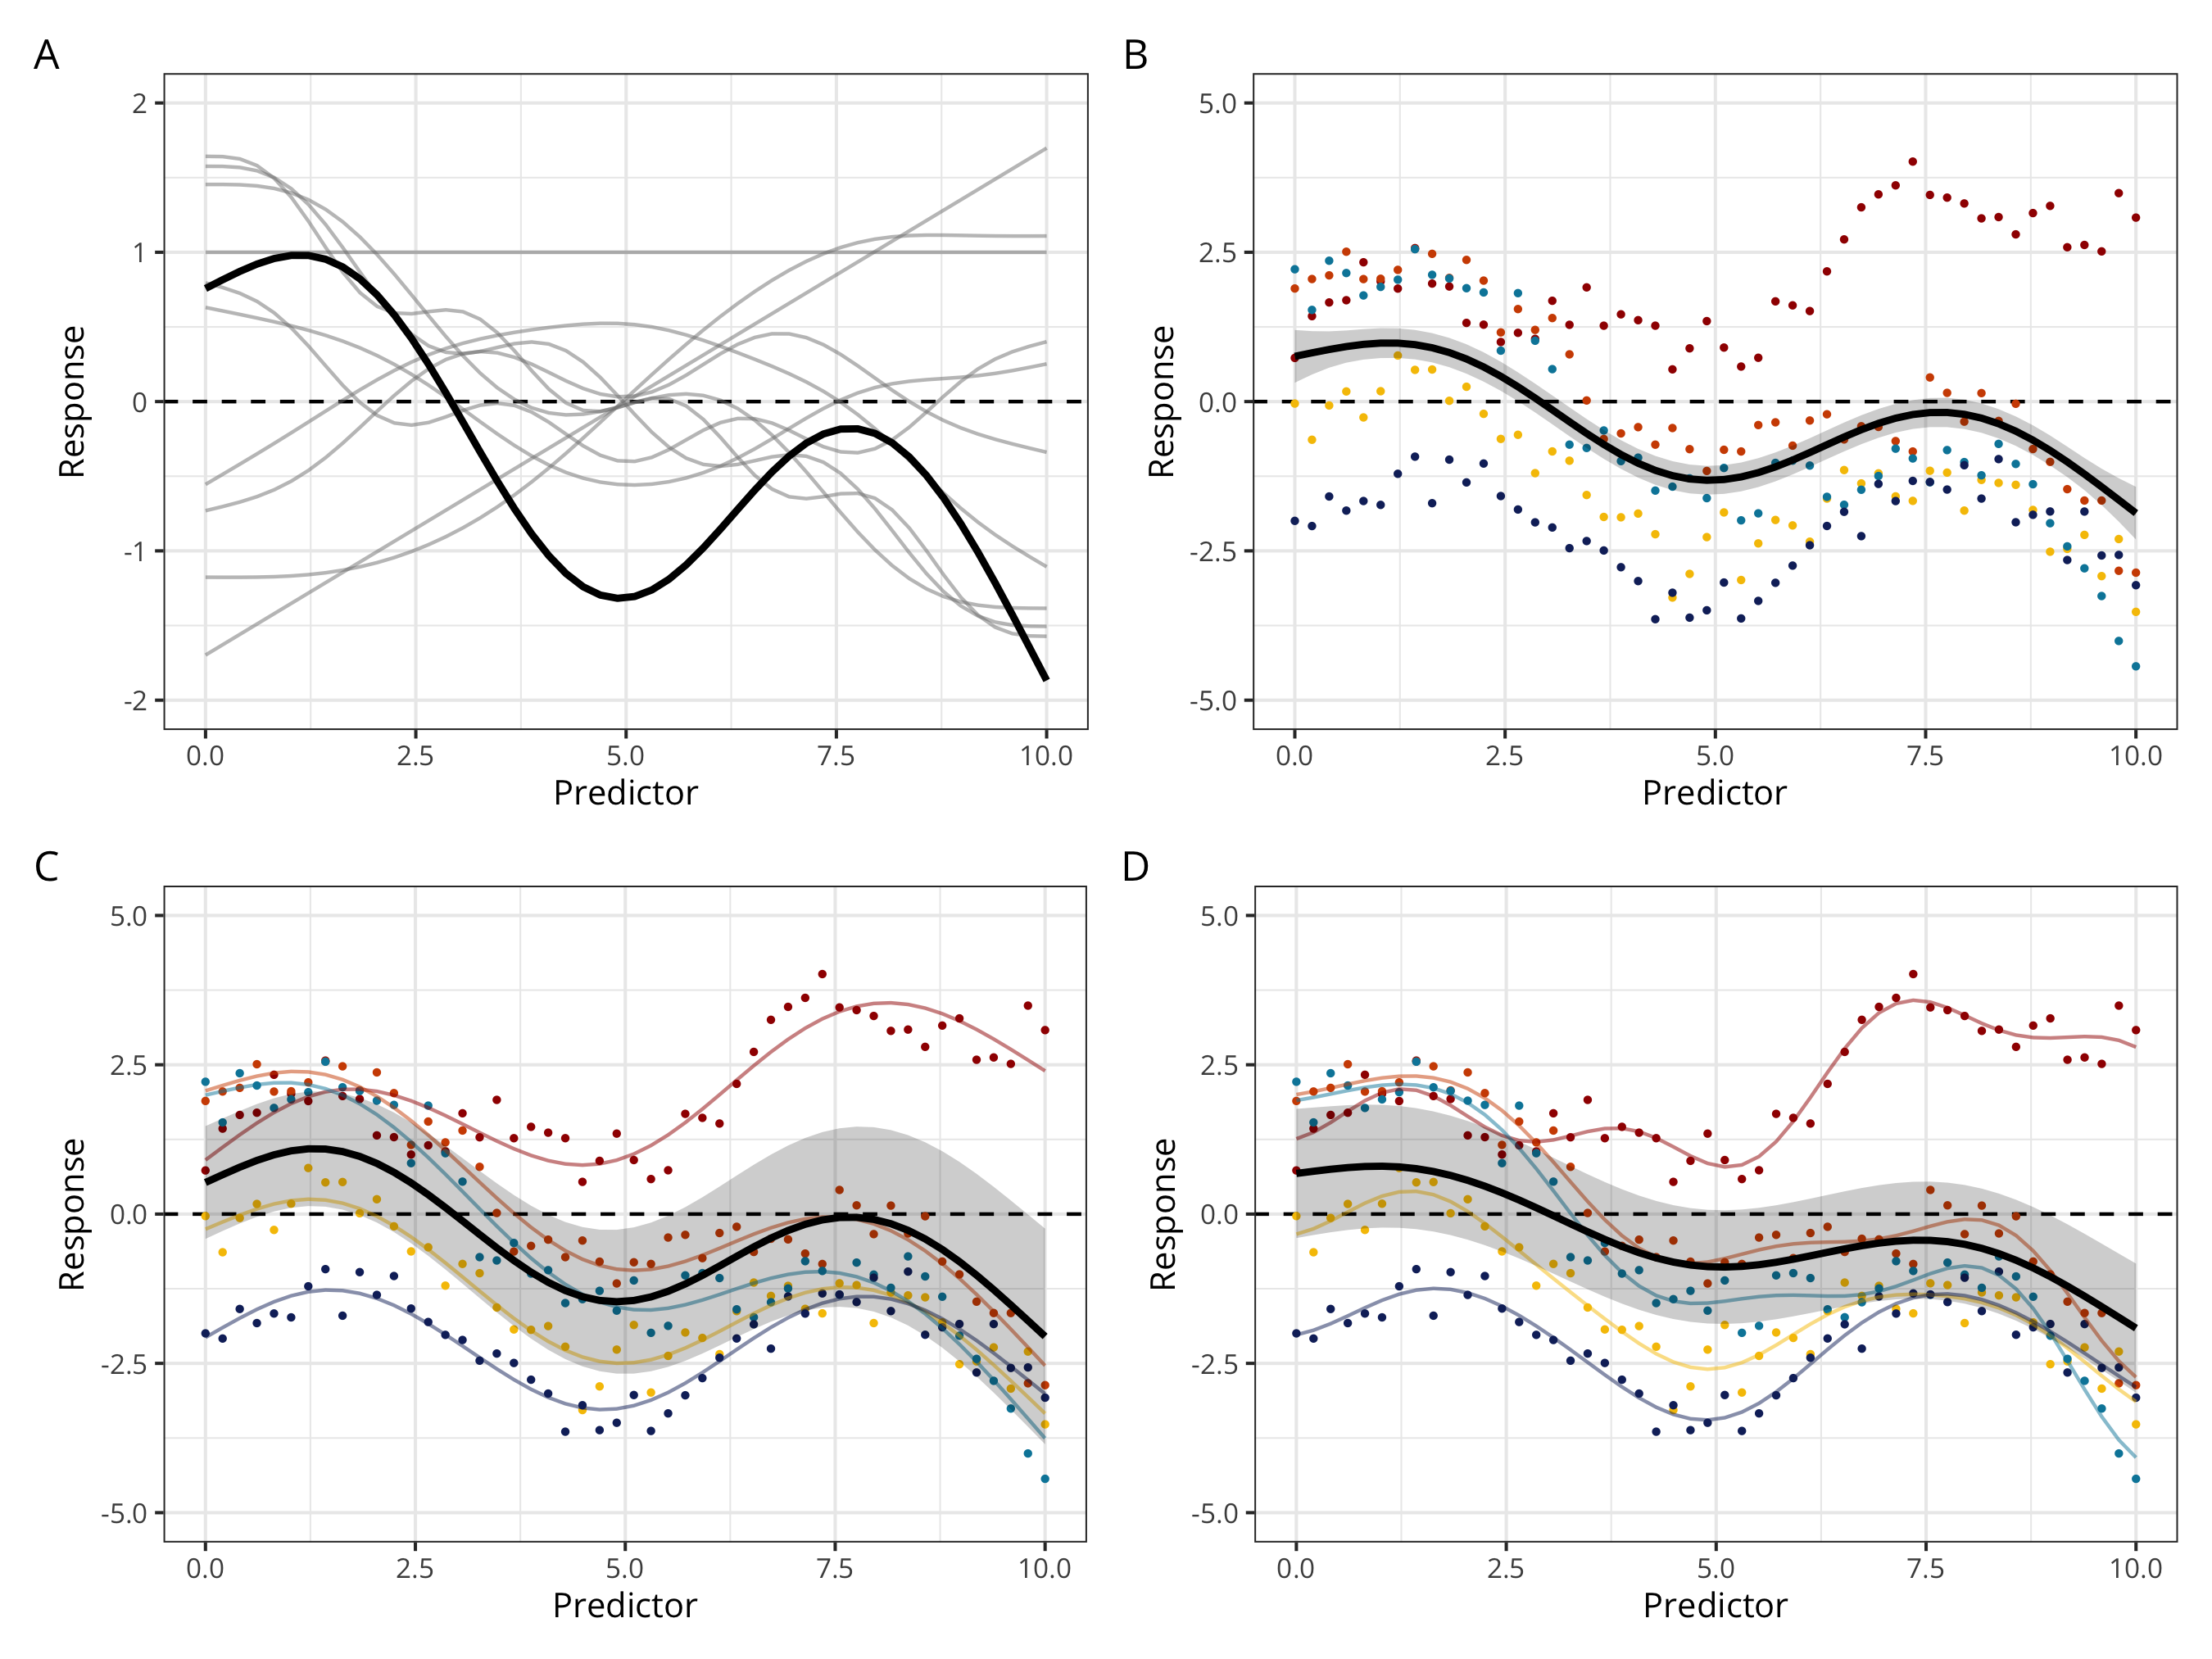
\includegraphics[width=1\textwidth,height=\textheight]{manuscript_files/figure-pdf/fig-intro-gam-1.png}

}

\end{figure}%

A detailed treatment of the technical underpinnings of GAMs is beyond
the scope of this article (see reference books such as
\citeproc{ref-hastie2017}{Hastie \& Tibshirani, 2017};
\citeproc{ref-wood2017}{Wood, 2017a}). However, it is worth emphasising
that GAMs have been successfully applied to a wide range of time series
data across the cognitive sciences, including pupillometry (e.g.,
\citeproc{ref-vanrij2019}{Rij et al., 2019}), articulography (e.g.,
\citeproc{ref-wieling2018}{Wieling, 2018}), speech formant dynamics
(e.g., \citeproc{ref-suxf3skuthy2021}{Sóskuthy, 2021}), neuroimaging
data (e.g., \citeproc{ref-dinga2021}{Dinga et al., 2021}), and
event-related potentials (e.g., \citeproc{ref-abugaber2023}{Abugaber et
al., 2023}; \citeproc{ref-baayen2018}{Baayen et al., 2018};
\citeproc{ref-meulman2015}{Meulman et al., 2015},
\citeproc{ref-meulman2023}{2023}). Their appeal for modelling M/EEG data
lies in their ability to flexibly capture the complex shape of ERP
waveforms without overfitting, through the use of smooth functions
constrained by penalisation. Recent extensions, such as distributional
GAMs (\citeproc{ref-rigby2005}{Rigby \& Stasinopoulos, 2005};
\citeproc{ref-umlauf2018}{Umlauf et al., 2018}), allow researchers to
model not only the mean structure but also the variance (or scale) and
other distributional properties as functions of predictors, a feature
that has proven useful in modelling neuroimaging data (e.g.,
\citeproc{ref-dinga2021}{Dinga et al., 2021}). Moreover, hierarchical or
multilevel GAMs (\citeproc{ref-pedersen_hierarchical_2019}{E. J.
Pedersen et al., 2019}) provide a principled way to account for the
nested structure of M/EEG data (e.g., trials within participants),
enabling the inclusion of varying intercepts, slopes, and smoothers (as
illustrated in Figure~\ref{fig-intro-gam}\ignorespaces C-D). This
approach mitigates the risk of overfitting and reduces the influence of
outliers on smooth estimates (\citeproc{ref-baayen2020}{Baayen \& Linke,
2020}; \citeproc{ref-meulman2023}{Meulman et al., 2023}).

\subsection{Objectives}\label{objectives}

Cluster-based permutation tests are widely used in M/EEG research to
identify statistically significant effects across time and space.
However, these methods have notable limitations, particularly in
accurately determining the precise onset and offset of neural effects.
To address these limitations, we developed a model-based approach
relying on Bayesian generalised additive multilevel models implemented
in \texttt{R} via the \texttt{brms} package
(\citeproc{ref-brms2017}{Bürkner, 2017}, \citeproc{ref-brms2018}{2018}).
We evaluated the performance of this approach against conventional
methods using both simulated and actual M/EEG data. Our findings
demonstrate that this method provides more precise and reliable
estimates of effects' onset and offset than conventional approaches such
as cluster-based inference.

\section{Benchmarking with known ground
truth}\label{benchmarking-with-known-ground-truth}

\subsection{Methods}\label{methods}

\subsubsection{M/EEG data simulation}\label{meeg-data-simulation}

To assess the accuracy of group-level onset and offset estimation of our
proposed method, we simulated EEG with known onset and offset values.
Following the approach of Sassenhagen \& Draschkow
(\citeproc{ref-sassenhagen2019}{2019}) and Rousselet
(\citeproc{ref-rousselet_using_2025}{2025}), we simulated EEG data
stemming from two conditions, one with noise only, and the other with
noise + signal. As in previous studies, the noise was generated by
superimposing 50 sinusoids at different frequencies, following an
EEG-like spectrum (see code in the online supplementary materials and
details in \citeproc{ref-yeung2004}{Yeung et al., 2004}). As in
Rousselet (\citeproc{ref-rousselet_using_2025}{2025}), the signal was
generated from a truncated Gaussian distribution with an objective onset
at 160 ms, a peak at 250 ms, and an offset at 342 ms. We simulated this
signal for 250 timesteps between 0 and 0.5s, akin to a 500 Hz sampling
rate. We simulated data for a group of 20 participants (with variable
true onset) with 50 trials per participant and condition
(Figure~\ref{fig-eeg}). All figures and simulation results can be
reproduced using the \texttt{R} code available online at:
\url{https://github.com/lnalborczyk/brms_meeg}.

\begin{figure}[!htb]

\caption{\label{fig-eeg}Mean simulated EEG activity in two conditions
with 50 trials each, for a group of 20 participants. The error band
represents the mean +/- 1 standard error of the mean.}

\centering{

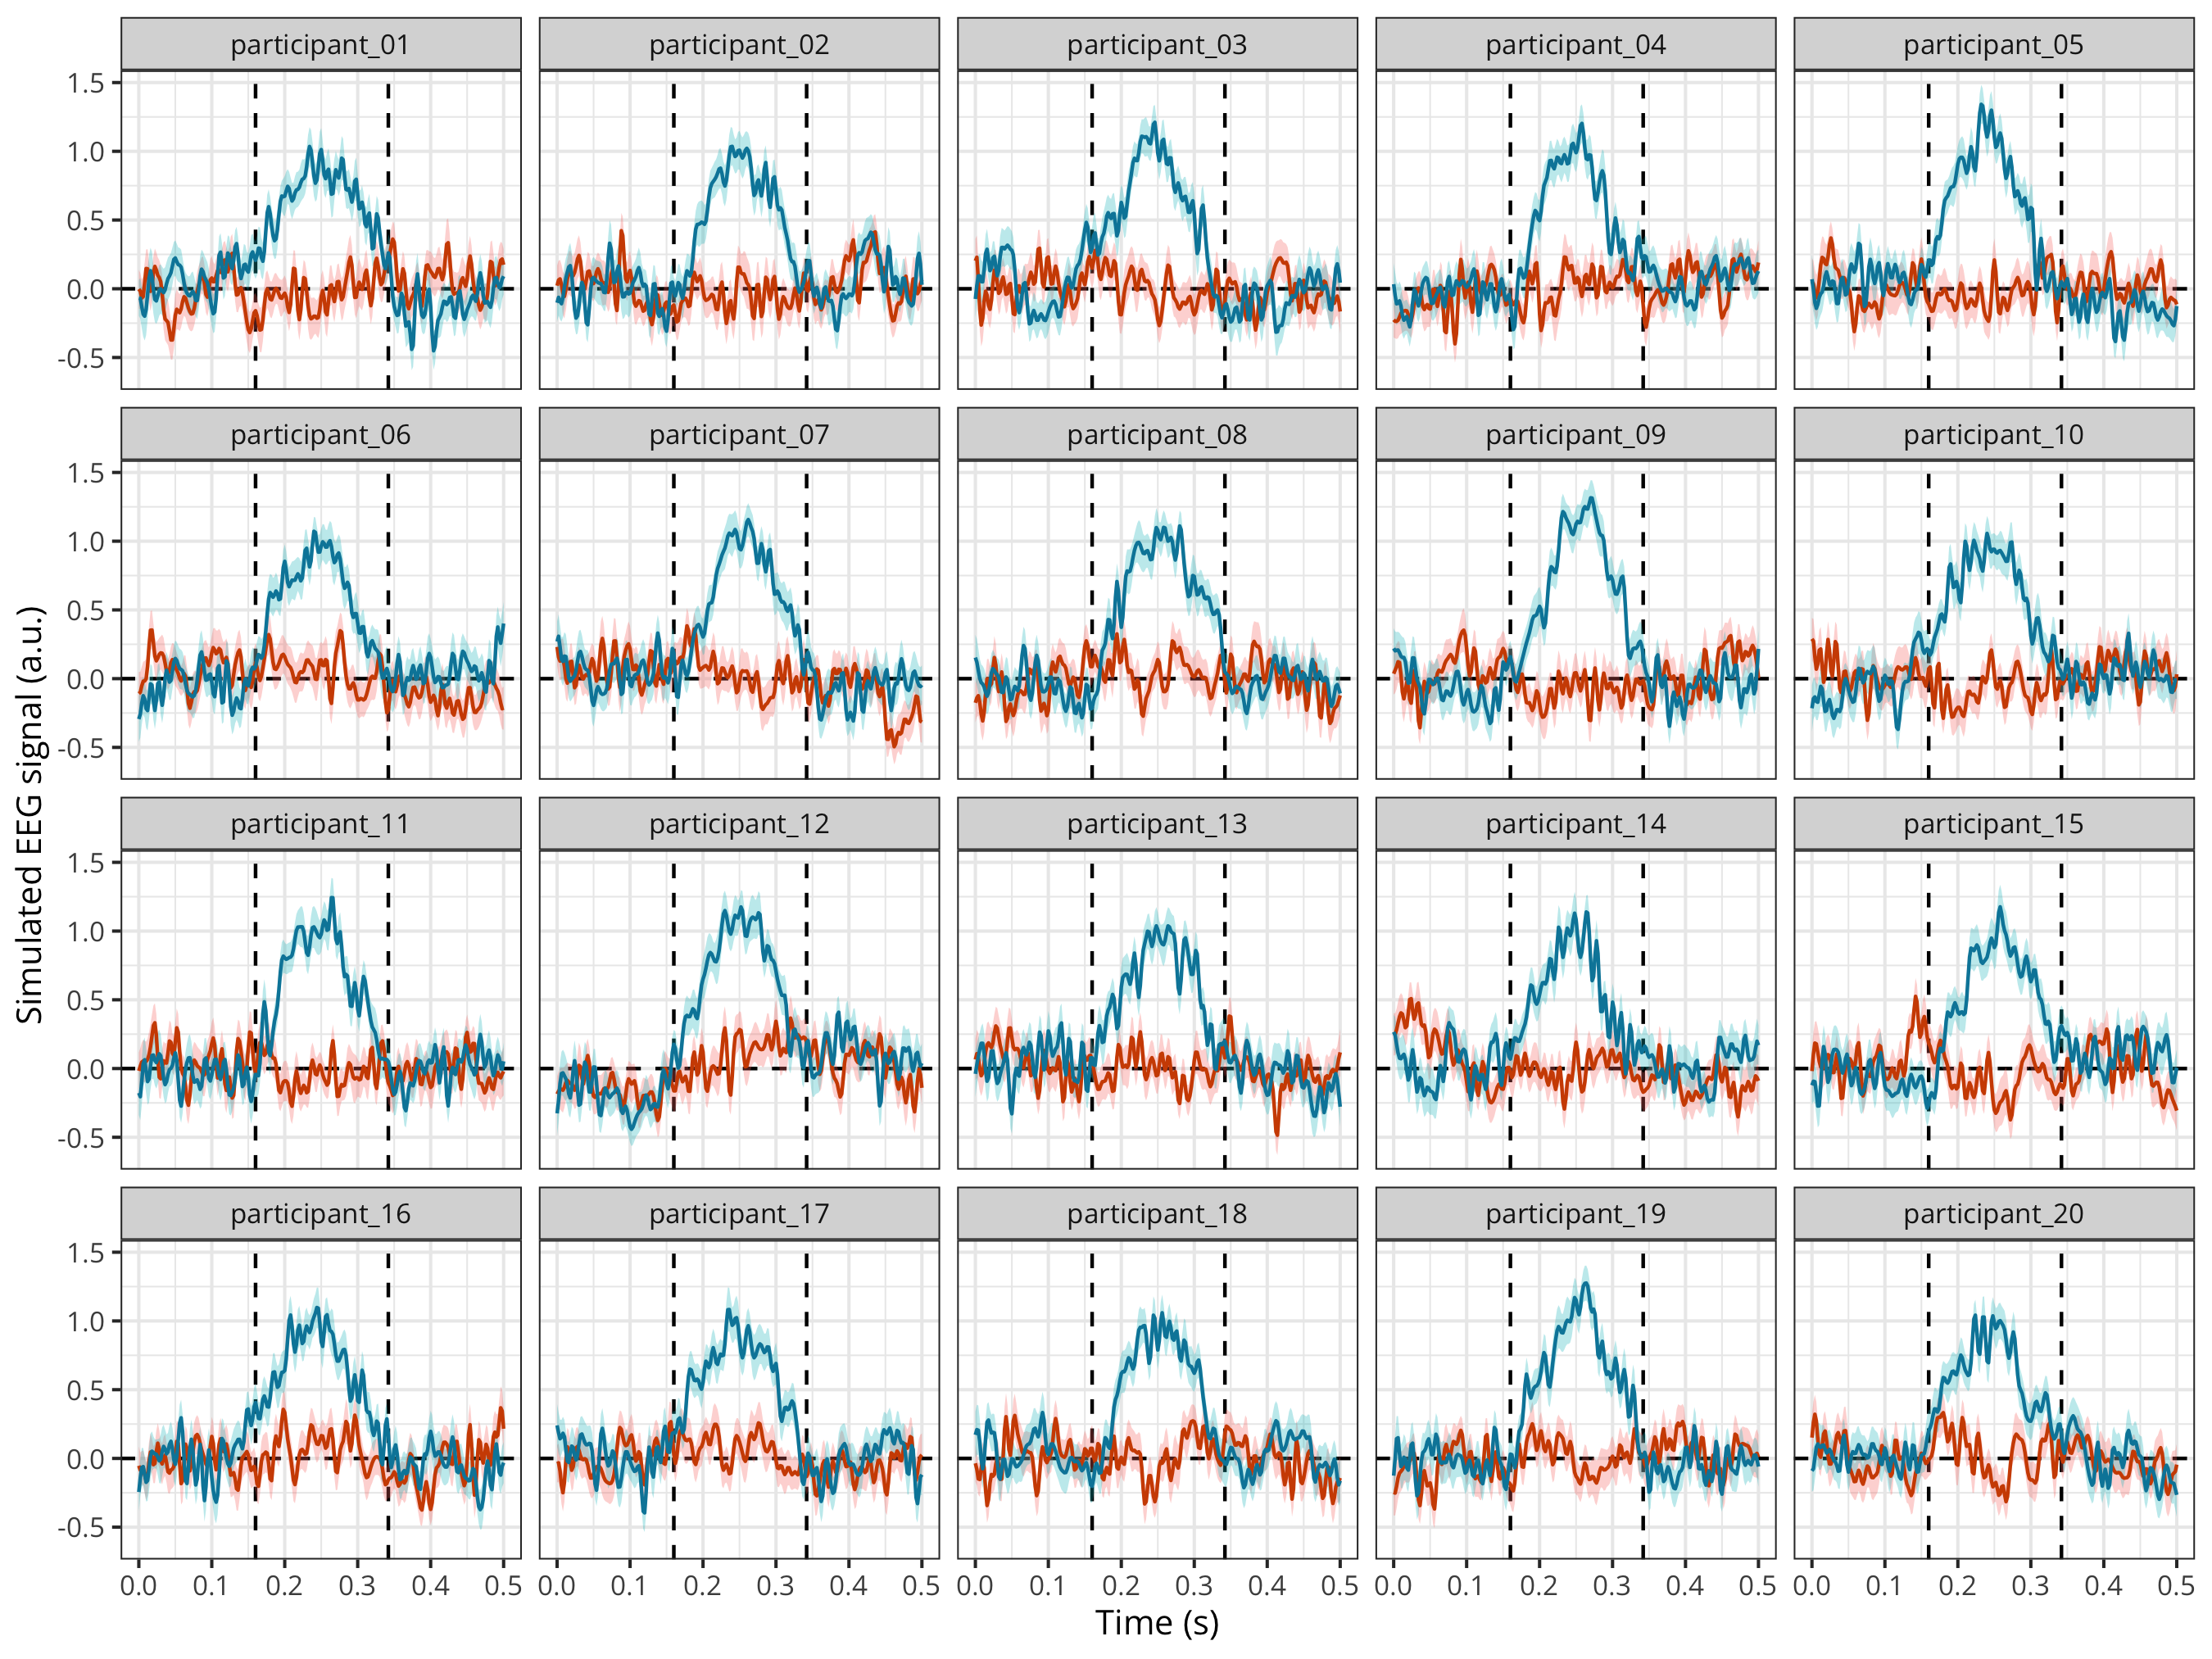
\includegraphics[width=1\textwidth,height=\textheight]{manuscript_files/figure-pdf/fig-eeg-1.png}

}

\end{figure}%

\subsubsection{Model description and model
fitting}\label{model-description-and-model-fitting}

We then fitted a Bayesian GAM (BGAM) using the \texttt{brms} package
(\citeproc{ref-brms2017}{Bürkner, 2017}, \citeproc{ref-brms2018}{2018})
and default priors (i.e., weakly informative priors). We ran eight
Markov Chain Monte-Carlo (MCMC) to approximate the posterior
distribution, including each 5000 iterations and a warmup of 2000
iterations, yielding a total of \(8 \times (5000-2000) = 24000\)
posterior samples to use for inference. Posterior convergence was
assessed examining trace plots as well as the Gelman--Rubin statistic
\(\hat{R}\) (\citeproc{ref-gabry2019}{Gabry et al., 2019};
\citeproc{ref-gelman2020}{Gelman et al., 2020};
\citeproc{ref-vehtari2021}{Vehtari et al., 2021}). The \texttt{brms}
package uses the same syntax as the \texttt{R} package \texttt{mgcv} v
1.9-3 (\citeproc{ref-mgcv}{Wood, 2017b}) for specifying smooth effects.
Figure~\ref{fig-plot-post-slope} shows the predictions of this model
together with the raw data.

However, the model whose predictions are depicted in
Figure~\ref{fig-plot-post-slope} only included constant (fixed) effects,
thus not properly accounting for between-participant variability. We
next fitted a multilevel version of the BGAM (BGAMM, for an introduction
to Bayesian multilevel models in \texttt{brms}, see
\citeproc{ref-nalborczyk2019}{Nalborczyk et al., 2019}) including a
varying intercept and slope for participant (but with a constant
smoother). Although it is possible to fit a BGAMM using data at the
single-trial level, we present a computationally lighter version of the
model that is fitted directly on by-participant summary statistics (mean
and SD), similar to what is done in meta-analysis.

We depict the posterior predictions together with the posterior estimate
of the slope for \texttt{condition} at each timestep
(Figure~\ref{fig-plot-post-slope}). This figure suggests that the BGAMM
provides an adequate description of the simulated data (see further
posterior predictive checks in \hyperref[apx-basis]{Appendix~B}).

\begin{figure}[!htb]

\caption{\label{fig-plot-post-slope}Posterior estimate of the EEG
activity in each condition (left) and posterior estimate of the
difference in EEG activity (right) according to the BGAMM.}

\centering{

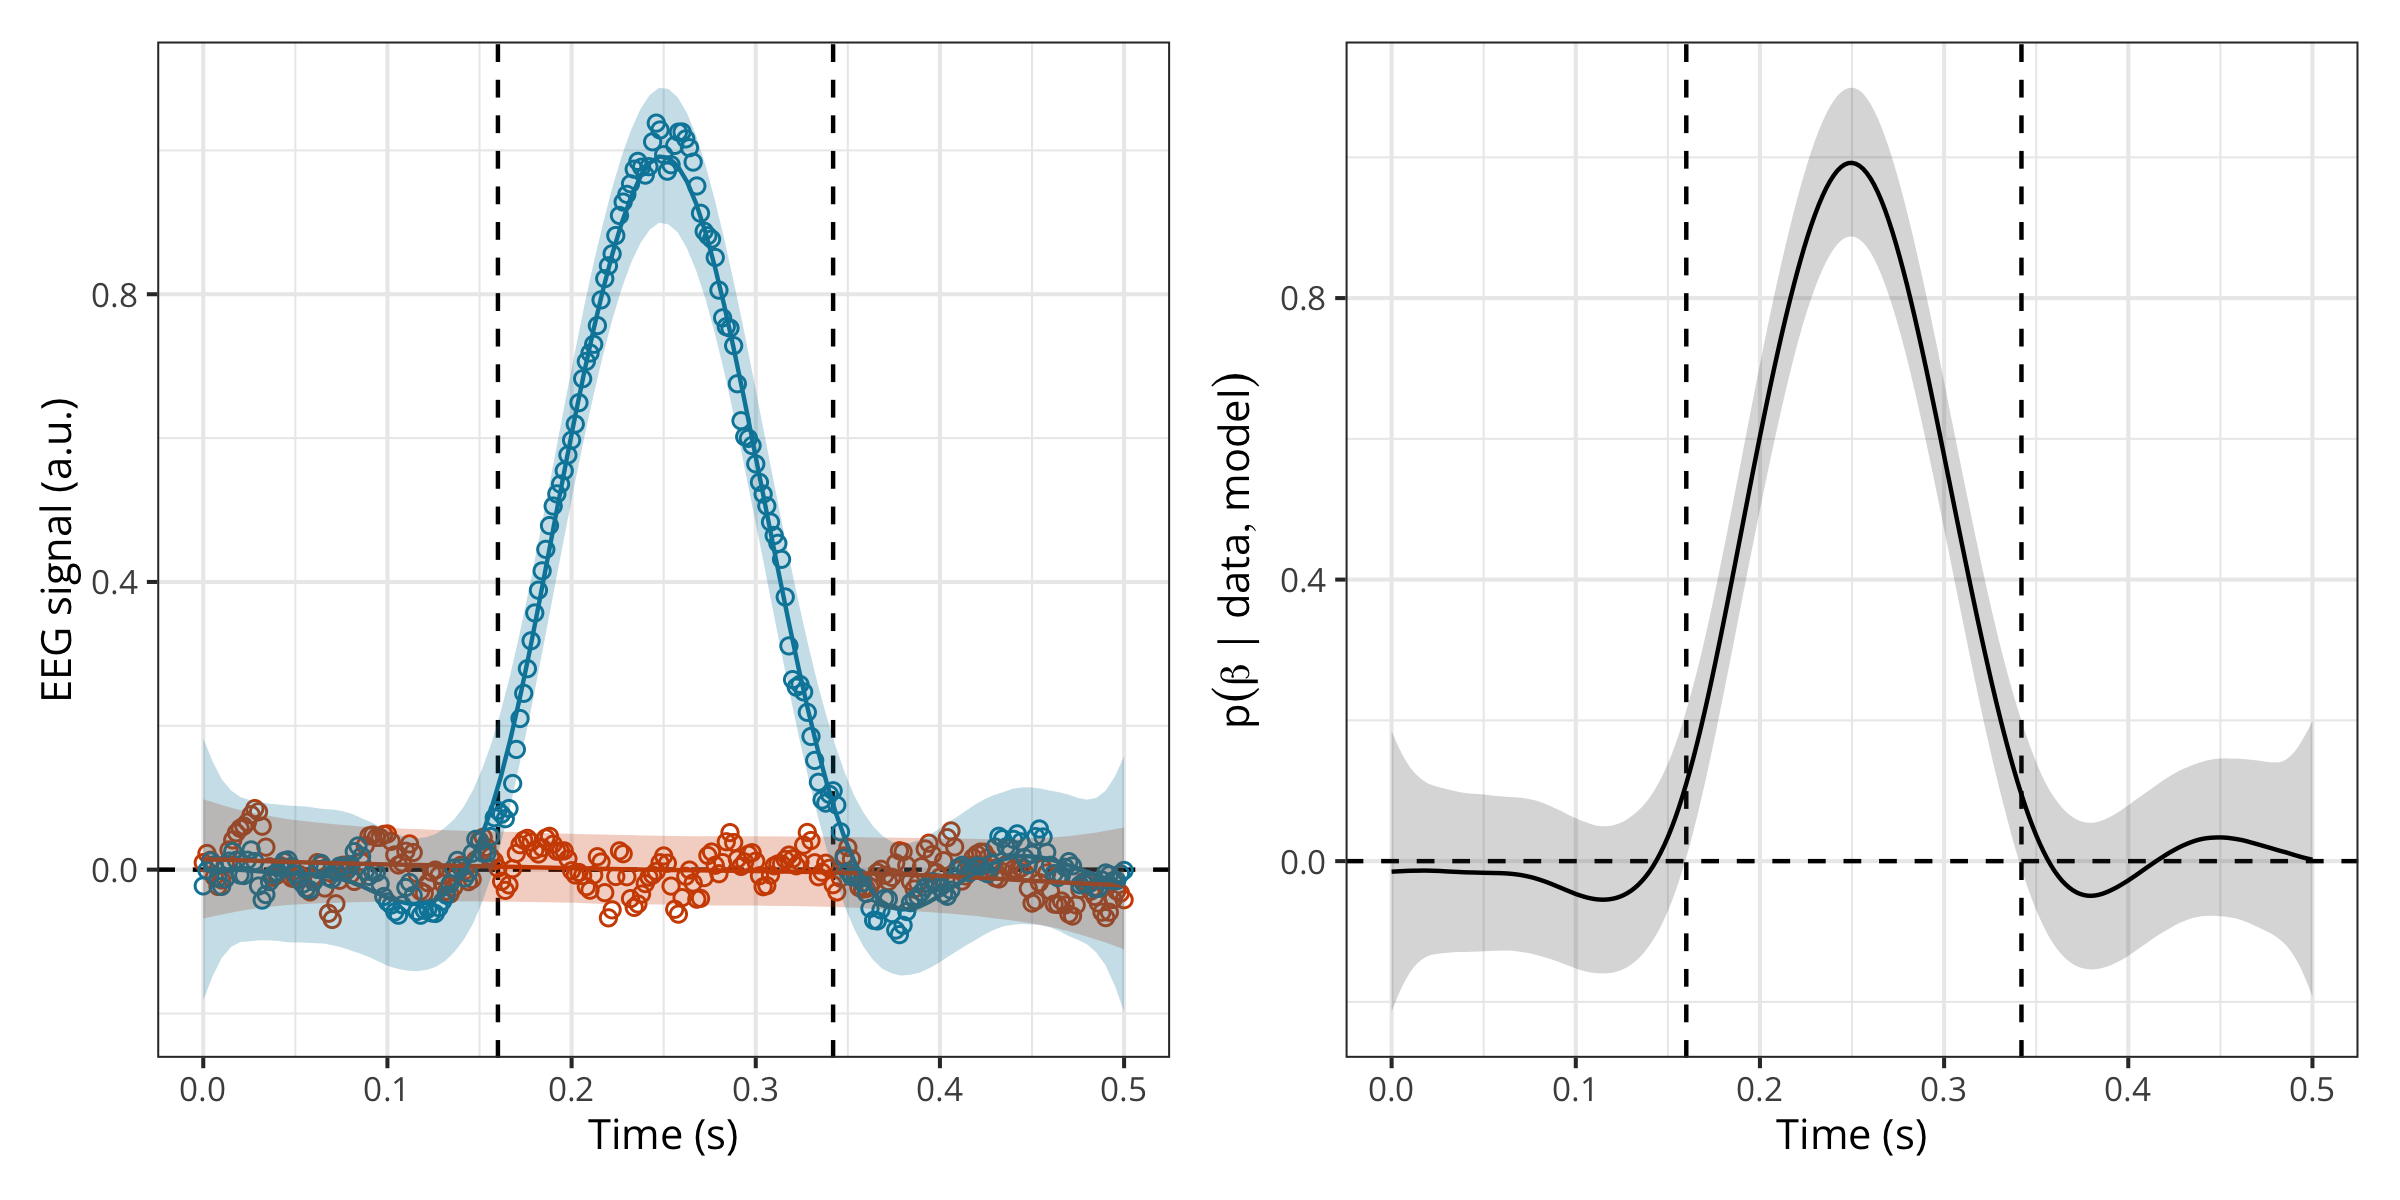
\includegraphics[width=1\textwidth,height=\textheight]{manuscript_files/figure-pdf/fig-plot-post-slope-1.png}

}

\end{figure}%

We then compute the posterior probability of the slope for
\texttt{condition} being above \(0\) (Figure~\ref{fig-post-prob-ratio},
left). From this quantity, we compute the ratio of posterior
probabilities (i.e., \(p/(1-p)\)), or posterior odds, and visualise the
timecourse of these odds superimposed with the conventional thresholds
on evidence ratios (Figure~\ref{fig-post-prob-ratio}, right). A ratio of
10 means that the probability of the difference being above 0 is 10
times higher than the probability of the difference not being above 0,
given the data, the priors, and other model's assumptions.\footnote{These
  posterior odds are equivalent to a Bayes factor, assuming 1:1 prior
  odds.} Thresholding the posterior odds thus provides a model-based
approach for estimating the onset and offset of M/EEG effects, whose
properties will be assessed in the simulation study. An important
advantage is that the proposed approach can be extended to virtually any
model structure.

\begin{figure}[!htb]

\caption{\label{fig-post-prob-ratio}Left: Posterior probability of the
EEG difference (slope) being above 0 according to the BGAMM. Right:
Posterior odds according to the BGAMM (on a log10 scale). Timesteps
above threshold (10) are highlighted in green. NB: the minimum and
maximum possible posterior odds are determined (bounded) by the number
of posterior samples in the model.}

\centering{

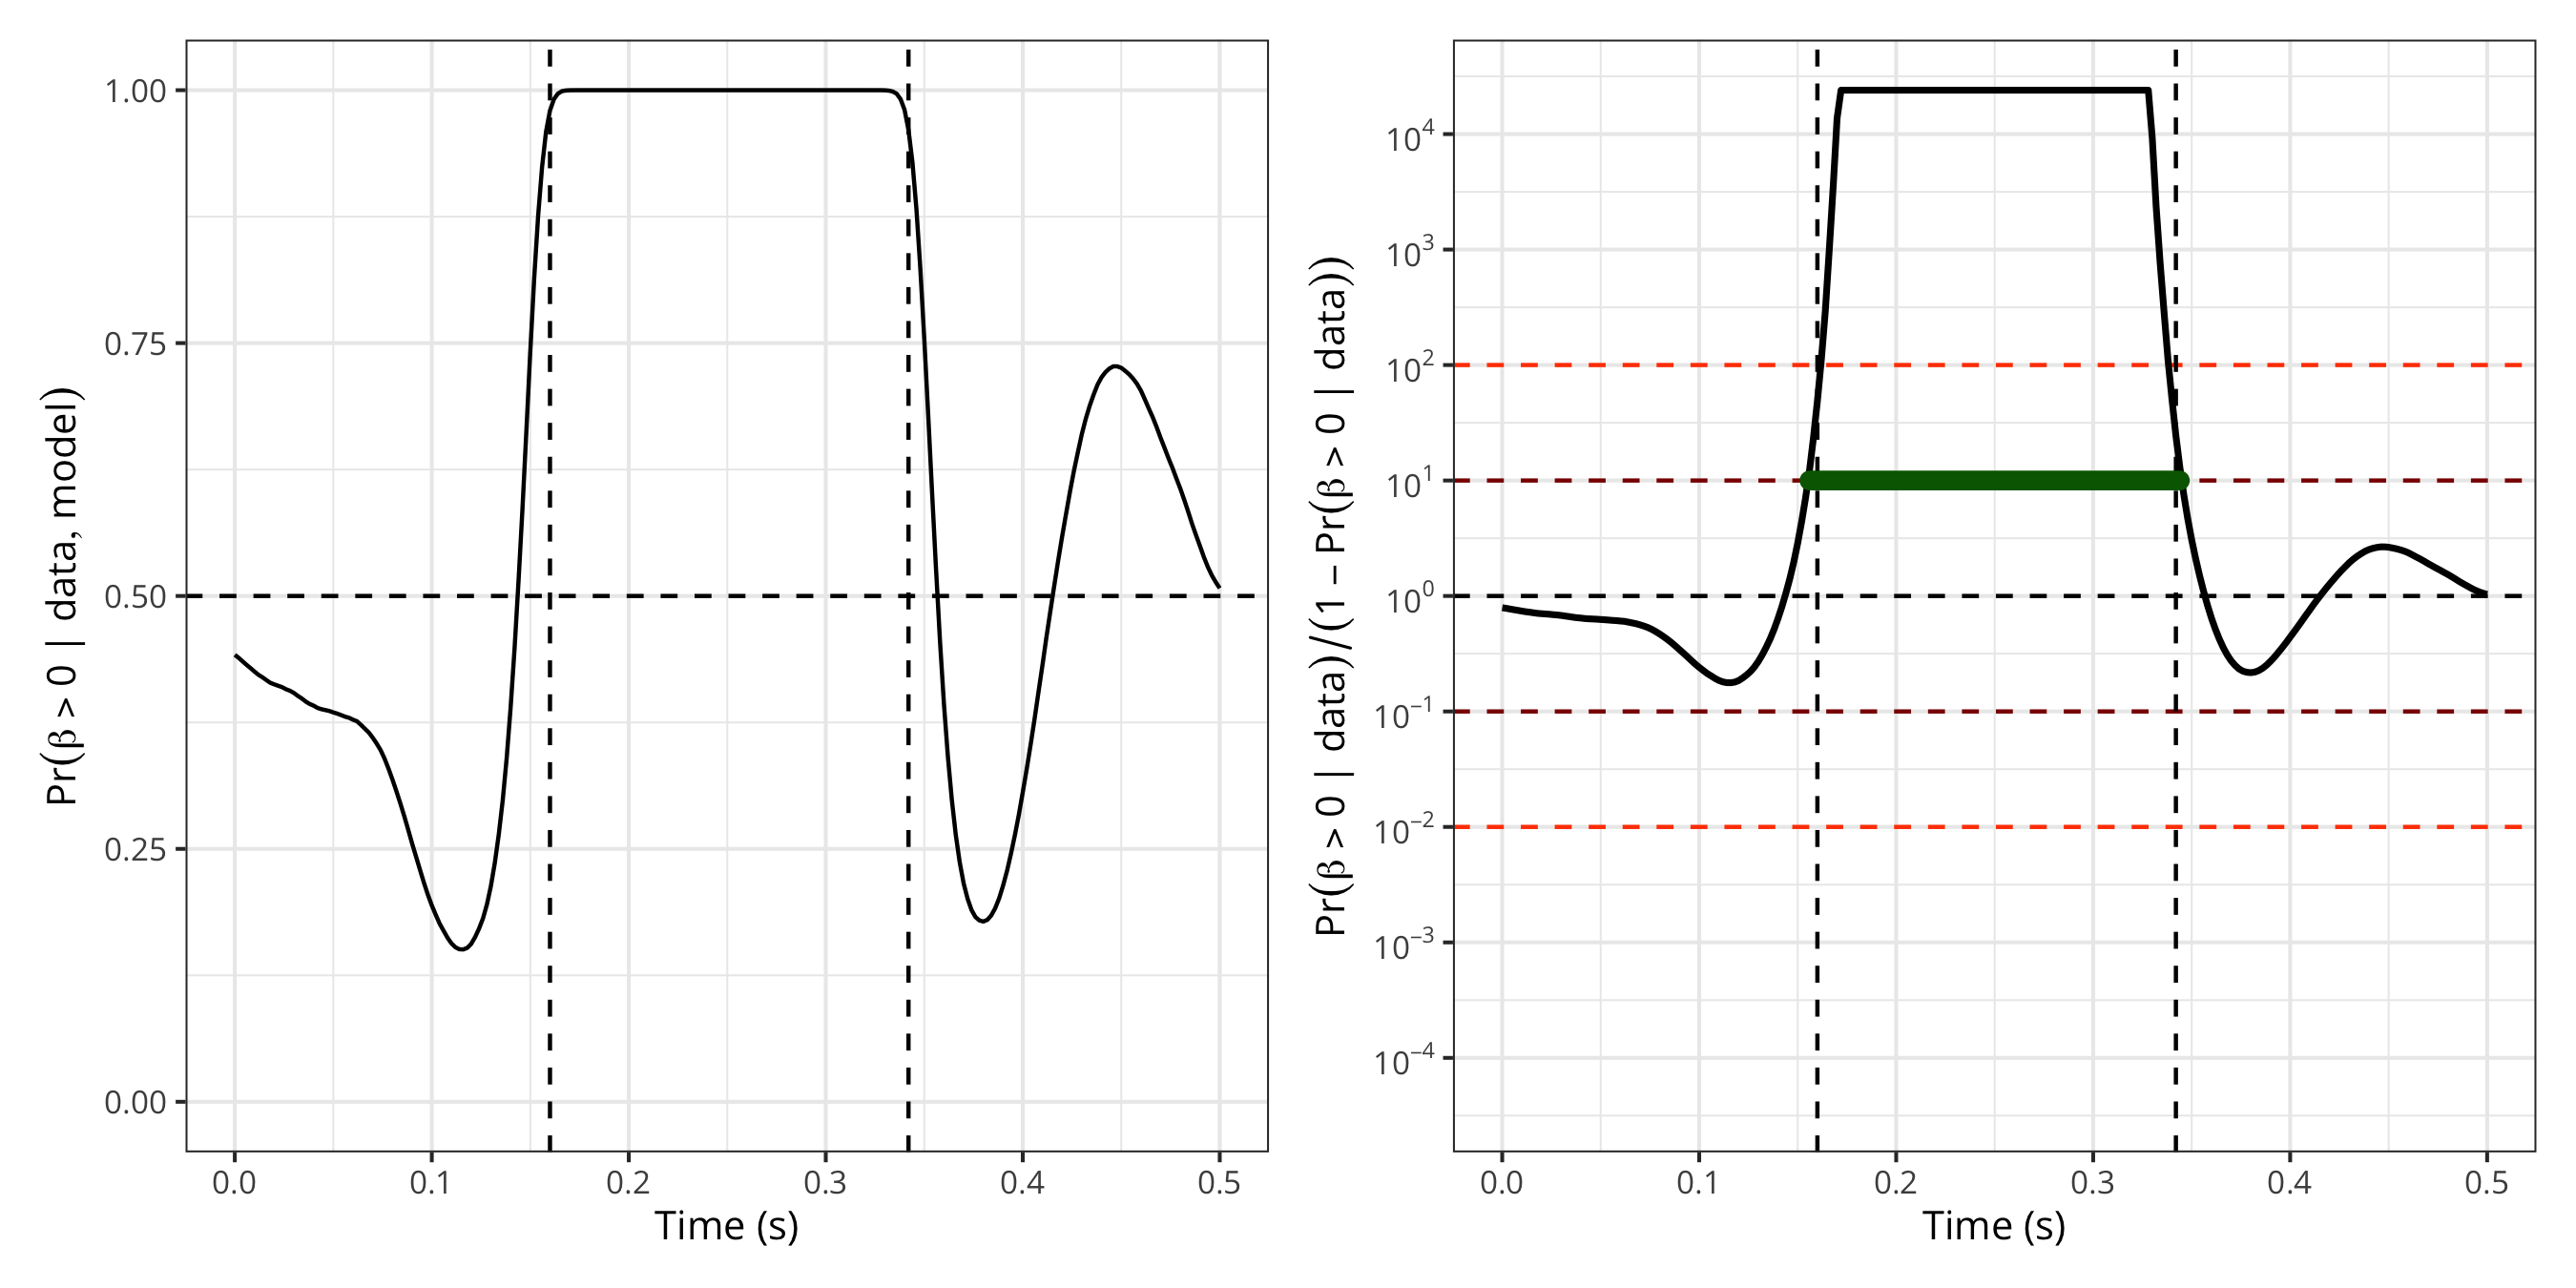
\includegraphics[width=1\textwidth,height=\textheight]{manuscript_files/figure-pdf/fig-post-prob-ratio-1.png}

}

\end{figure}%

\subsubsection{Comparing the onset/offset estimates across
approaches}\label{comparing-the-onsetoffset-estimates-across-approaches}

We then compared the ability of the BGAM to accurately estimate the
onset and offset of the ERP difference to other widely-used methods.
First, we conducted mass-univariate t-tests (thus treating each timestep
independently) and identified the onset and offset of the ERP difference
as the first and last values crossing an arbitrary significance
threshold (\(\alpha = 0.05\)). We then followed the same approach but
after applying different forms of multiplicity correction to the
\(p\)-values. We compared two methods that control the FDR (i.e.,
\texttt{BH95}, \citeproc{ref-benjamini1995}{Benjamini \& Hochberg,
1995}; and \texttt{BY01}, \citeproc{ref-benjamini2001}{Benjamini \&
Yekutieli, 2001}), one method that controls the FWER (i.e.,
Holm--Bonferroni method, \citeproc{ref-holm1979}{Holm, 1979}), and two
cluster-based permutation methods (permutation with a single
cluster-forming threshold and threshold-free cluster enhancement,
\texttt{TFCE}, \citeproc{ref-smith2009}{S. Smith \& Nichols, 2009}). The
\texttt{BH95}, \texttt{BY01}, and \texttt{Holm} corrections were applied
to the p-values using the \texttt{p.adjust()} function in \texttt{R}.
The cluster-based inference was implemented using a cluster-sum
statistic of squared \(t\)-values, as implemented in \texttt{MNE-Python}
(\citeproc{ref-gramfort2013}{Gramfort, 2013}), called via the \texttt{R}
package \texttt{reticulate} v 1.42.0 (\citeproc{ref-reticulate}{Ushey et
al., 2024}). We also compared these estimates to the onset and offset as
estimated using the binary segmentation algorithm, as implemented in the
\texttt{R} package \texttt{changepoint} v 2.3
(\citeproc{ref-changepoint}{Killick et al., 2022}), and applied directly
to the squared \(t\)-values (as in
\citeproc{ref-rousselet_using_2025}{Rousselet, 2025}).\footnote{As in
  Rousselet (\citeproc{ref-rousselet_using_2025}{2025}), we fixed the
  number of expected change points to two in the binary segmentation
  algorithm, thus producing always one cluster.}
Figure~\ref{fig-corrections} illustrates the onsets and offsets
estimated by each method on a single simulated dataset and shows that
all methods systematically overestimate the true onset and underestimate
the true offset. In addition, the \texttt{Raw\ p-value},
\texttt{FDR\ BH95}, and \texttt{FDR\ BY01} methods identify clusters
well before the true onset and after the true offset.

\begin{figure}[!htb]

\caption{\label{fig-corrections}Exemplary timecourse of squared t-values
with true onset and offset (vertical black dashed lines) and
onsets/offsets identified using the raw p-values, the corrected p-values
(BH95, BY01, Holm), the cluster-based methods (Cluster mass, TFCE), or
using the binary segmentation method (Change point).}

\centering{

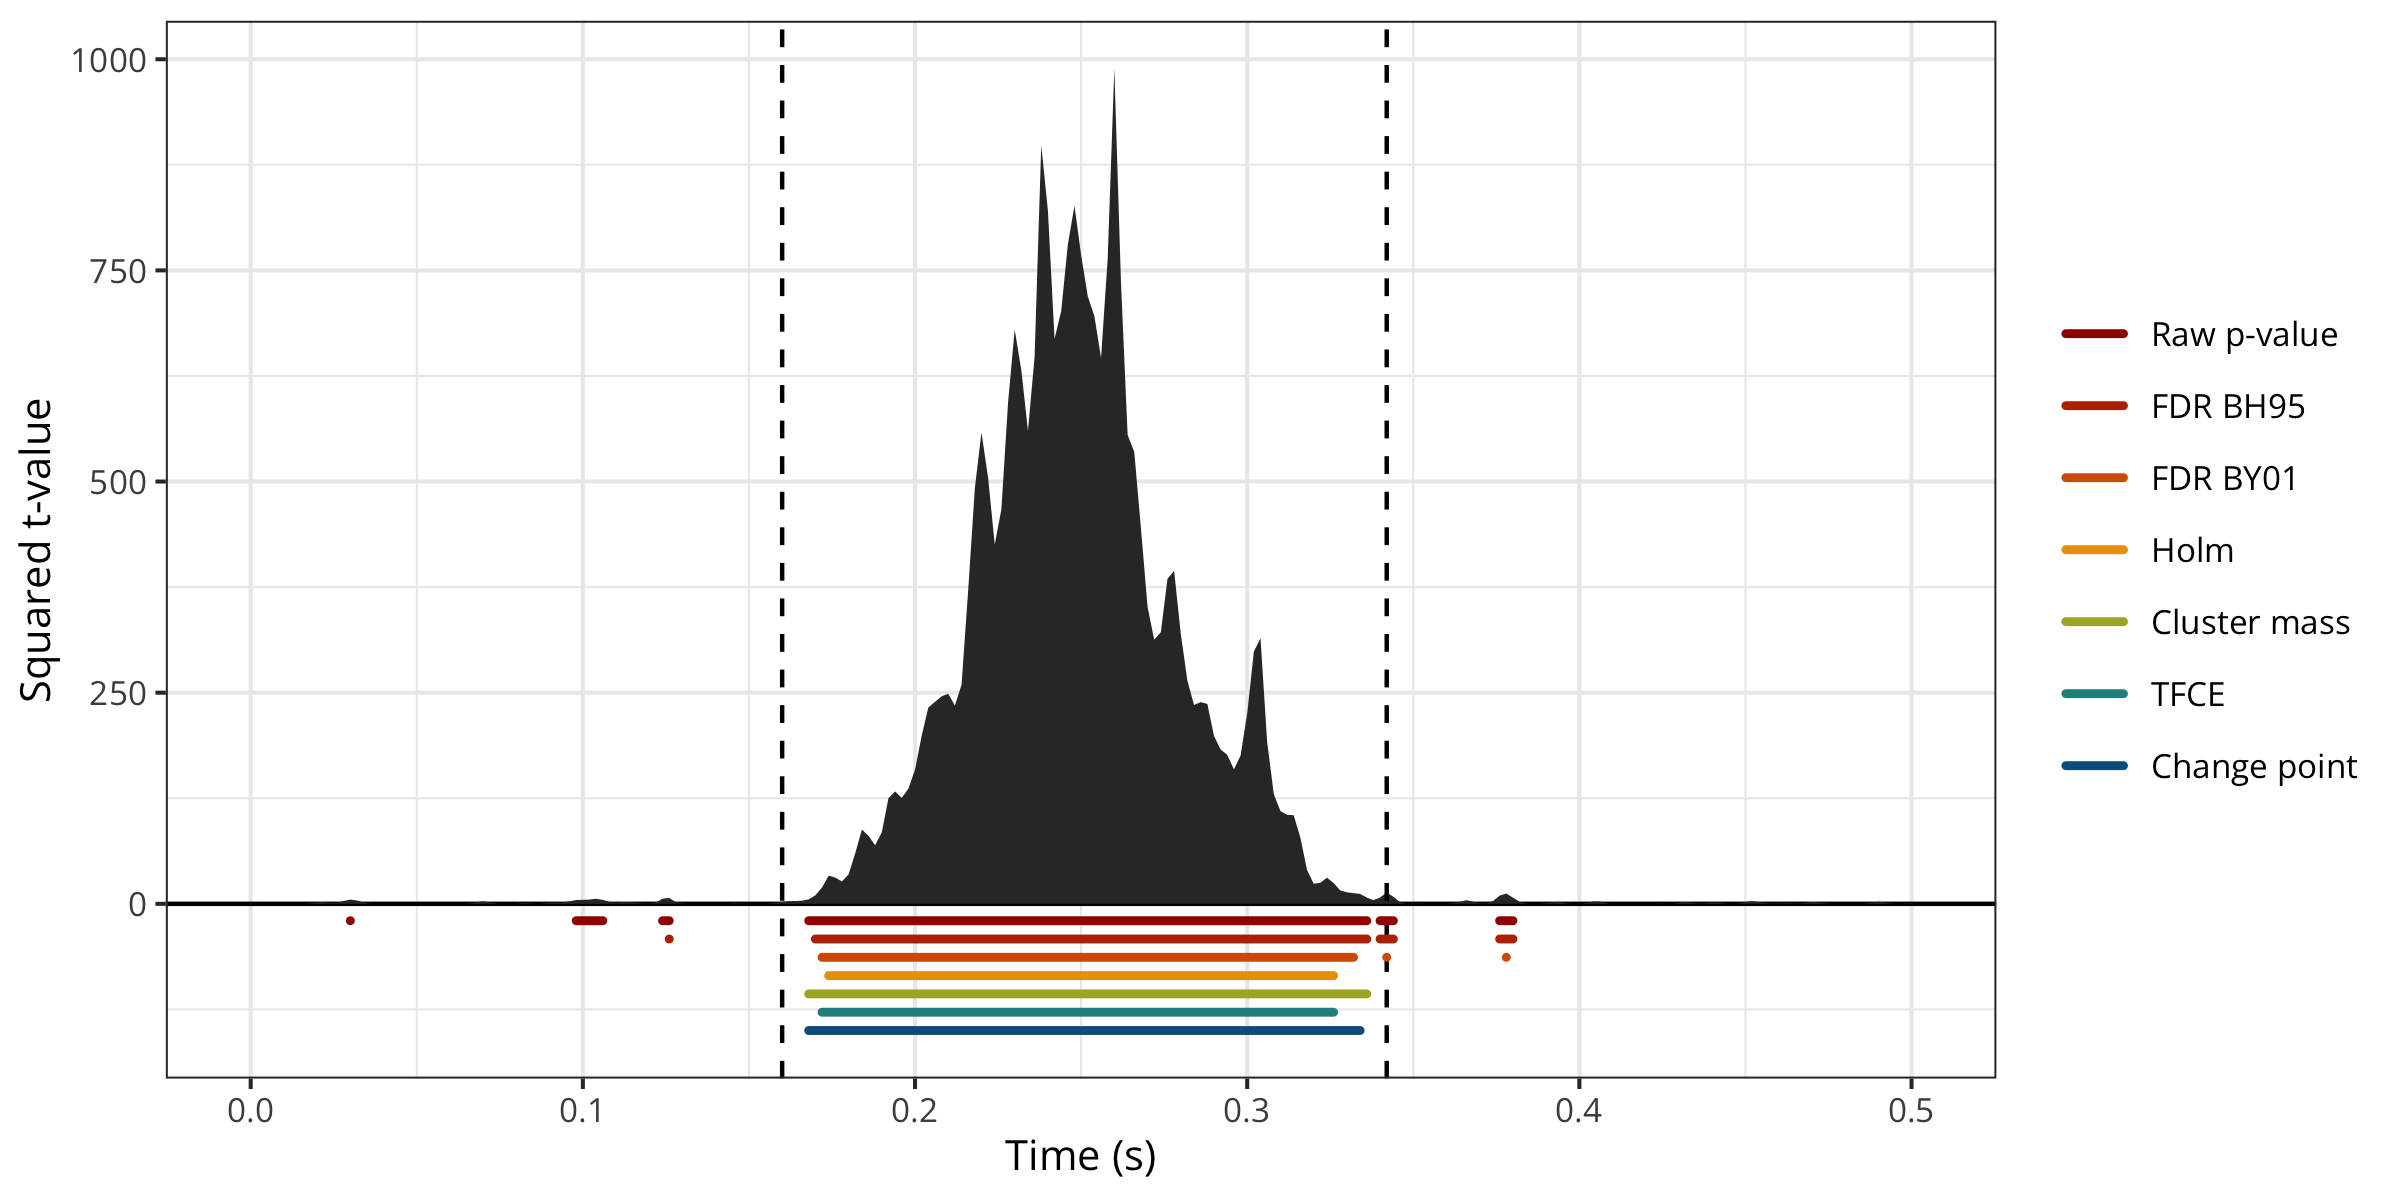
\includegraphics[width=1\textwidth,height=\textheight]{manuscript_files/figure-pdf/fig-corrections-1.png}

}

\end{figure}%

\subsubsection{Simulation study}\label{simulation-study}

To assess the accuracy of group-level onset and offset estimation, all
methods were compared by computing the bias (defined as the mean
difference between the estimated and true value of the onset/offset),
mean absolute error (MAE), root mean square error (RMSE), and variance
of onset/offset estimates from 10,000 simulated datasets. Following
Rousselet (\citeproc{ref-rousselet_using_2025}{2025}), each participant
was assigned a random onset between 150 and 170ms. Whereas the present
article focuses on one-dimensional signals (e.g., one M/EEG channel), we
provide a 2D application in \hyperref[apx-2D]{Appendix~A}.

\subsection{Results}\label{results}

Figure~\ref{fig-simulation-results} shows a summary of the simulation
results, revealing that the proposed approach (\texttt{BGAM}) has the
lowest error for both the onset and offset estimates. The
\texttt{Cluster\ mass} and \texttt{Change\ point} methods also have good
performance, but perhaps surprisingly, the \texttt{TFCE} method performs
poorly for estimating the offset of the effect (with performance similar
to the \texttt{Holm} method). Unsurprisingly, the \texttt{FDR\ BH95} and
\texttt{Raw\ p-value} methods show the worst performance.

\begin{figure}[!htb]

\caption{\label{fig-simulation-results}Mean error and variance of onset
and offset estimates according to each method. Variance is plotted on a
log10 scale for visual purposes.}

\centering{

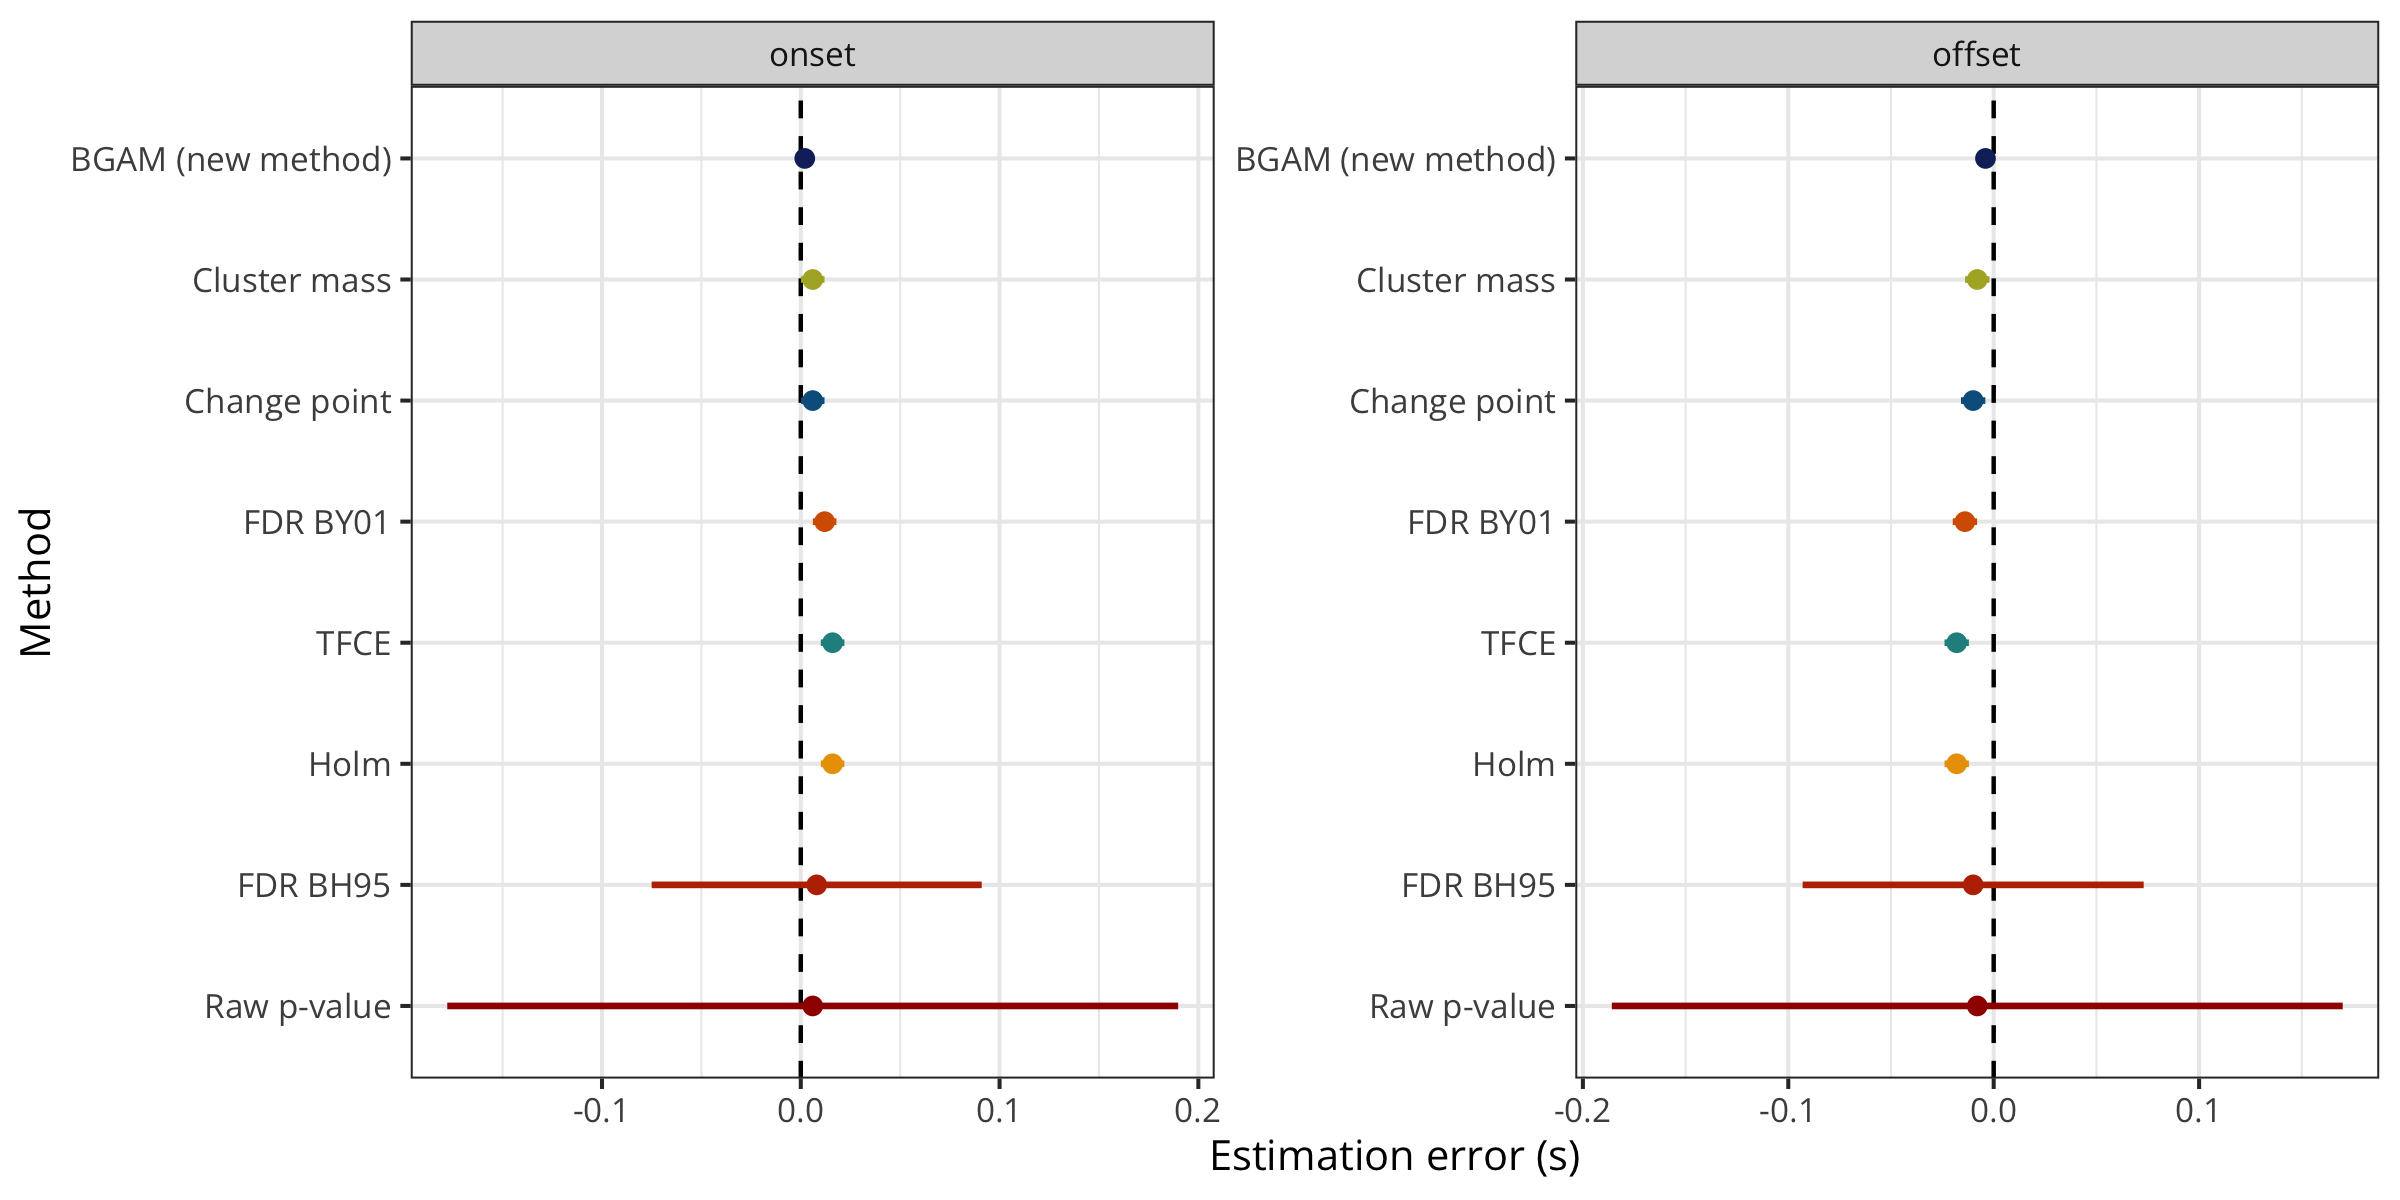
\includegraphics[width=1\textwidth,height=\textheight]{manuscript_files/figure-pdf/fig-simulation-results-1.png}

}

\end{figure}%

These results are further summarised in
Table~\ref{tbl-simulation-results}, which shows that the \texttt{BGAM}
method is almost perfectly unbiased (i.e., it has a bias of
approximately 0.1ms for the onset and 2.4ms for the offset). The
\texttt{Bias} column shows that all methods tend to estimate the onset
later than the true onset and to estimate the offset earlier than the
true offset. As can be seen from this table, the \texttt{BGAM} method
has the best performance on all included metrics (except for the
\texttt{Variance} of the offset estimate, where the
\texttt{Change\ point} method performs better, presumably because it was
constrained to identifying a single cluster).

\begin{table}

{\caption{{Summary statistics of onset/offset estimates for each method
(in ms, ordered by the MAE).}{\label{tbl-simulation-results}}}}

\fontsize{9.0pt}{10.8pt}\selectfont
\begin{tabular*}{\linewidth}{@{\extracolsep{\fill}}lcccc}
\toprule
 & Bias & MAE & RMSE & Variance \\ 
\midrule\addlinespace[2.5pt]
\multicolumn{5}{l}{onset} \\[2.5pt] 
\midrule\addlinespace[2.5pt]
BGAM (our method) & {\bfseries 0.11} & {\bfseries 2.76} & {\bfseries 0.11} & {\bfseries 28.78} \\ 
Change point & 5.17 & 6.51 & 5.17 & 33.58 \\ 
Cluster mass & 6.64 & 7.62 & 6.64 & 207.86 \\ 
Holm & 29.83 & 32.01 & 29.83 & 2,763.68 \\ 
TFCE & 29.73 & 32.07 & 29.73 & 2,823.11 \\ 
FDR BY01 & 36.67 & 50.80 & 36.67 & 7,872.30 \\ 
FDR BH95 & 58.64 & 102.49 & 58.64 & 19,054.58 \\ 
Raw p-value & 70.72 & 132.86 & 70.72 & 25,004.65 \\ 
\midrule\addlinespace[2.5pt]
\multicolumn{5}{l}{offset} \\[2.5pt] 
\midrule\addlinespace[2.5pt]
BGAM (our method) & {\bfseries -2.35} & {\bfseries 3.46} & {\bfseries 2.35} & 53.63 \\ 
Cluster mass & -8.64 & 9.44 & 8.64 & 193.63 \\ 
Change point & -9.28 & 9.82 & 9.28 & {\bfseries 33.03} \\ 
Holm & -31.86 & 34.03 & 31.86 & 2,764.12 \\ 
TFCE & -31.84 & 34.19 & 31.84 & 2,834.11 \\ 
FDR BY01 & -36.68 & 51.37 & 36.68 & 7,648.53 \\ 
FDR BH95 & -58.87 & 102.63 & 58.87 & 18,939.58 \\ 
Raw p-value & -72.93 & 133.33 & 72.93 & 25,012.72 \\ 
\bottomrule
\end{tabular*}

\end{table}

\section{Application to actual MEG
data}\label{application-to-actual-meg-data}

\subsection{Methods}\label{methods-1}

To complement the simulation study, we evaluated the performance of all
methods on actual MEG data (\citeproc{ref-nalborczyk:inprep}{Nalborczyk
et al., in preparation}). In this study, the authors conducted
time-resolved multivariate pattern analysis (MVPA, also known as
decoding) of MEG data recorded in 32 human participants during a reading
task. As a result, the authors obtained a timecourse of decoding accuray
(ROC AUC), bounded between 0 and 1, for each participant. To test
whether the group-level average decoding accuracy was above chance
(i.e., 0.5) at each timestep, we fitted a BGAM as introduced previously
with a basis dimension \(k=50\) and retained all timesteps exceeding a
posterior odds of 20. To better distinguish signal from noise, we
defined a region of practical equivalence (ROPE,
\citeproc{ref-kruschke2017}{Kruschke \& Liddell, 2017}) as the upper
90\% quantile of decoding performance during the baseline period (i.e.,
before stimulus onset). Although we chose a basis dimension of \(k=50\),
which seemed appropriate for the present data, this choice should be
adapted according to the properties of the modelled data (e.g.,
signal-to-noise ratio, prior low-pass filtering, sampling rate) and
should be assessed by the usual model checking tools (e.g., models
comparison, posterior predictive checks, see
\hyperref[apx-basis]{Appendix~B}).

\subsection{Results}\label{results-1}

Figure~\ref{fig-onset-offset} shows the group-level average decoding
performance through time superimposed with onset and offset estimates
from each method. Overall, this figure shows that both the
\texttt{Raw\ p-value} and \texttt{FDR\ BH95} methods are extremely
lenient, identifying clusters of above-chance decoding accuracy before
the onset of the stimulus (false positive) and until the end of the
trial. The \texttt{Change\ point} method seems to be the most
conservative one, identifying a single cluster spanning from
approximately +60ms to +450ms. The \texttt{Holm},
\texttt{Cluster\ mass}, \texttt{TFCE}, and \texttt{BGAM} methods produce
roughly similar estimates of onset and offset, ranging from
approximately +60ms to +650ms (considering only the first and last
identified timesteps), although the \texttt{BGAM} method seems to result
in fewer clusters.

\begin{figure}[!htb]

\caption{\label{fig-onset-offset}Group-level average decoding
performance through time with clusters of higher-than-chance decoding
performance as identified by each method (data from
\citeproc{ref-nalborczyk:inprep}{Nalborczyk et al., in preparation}).}

\centering{

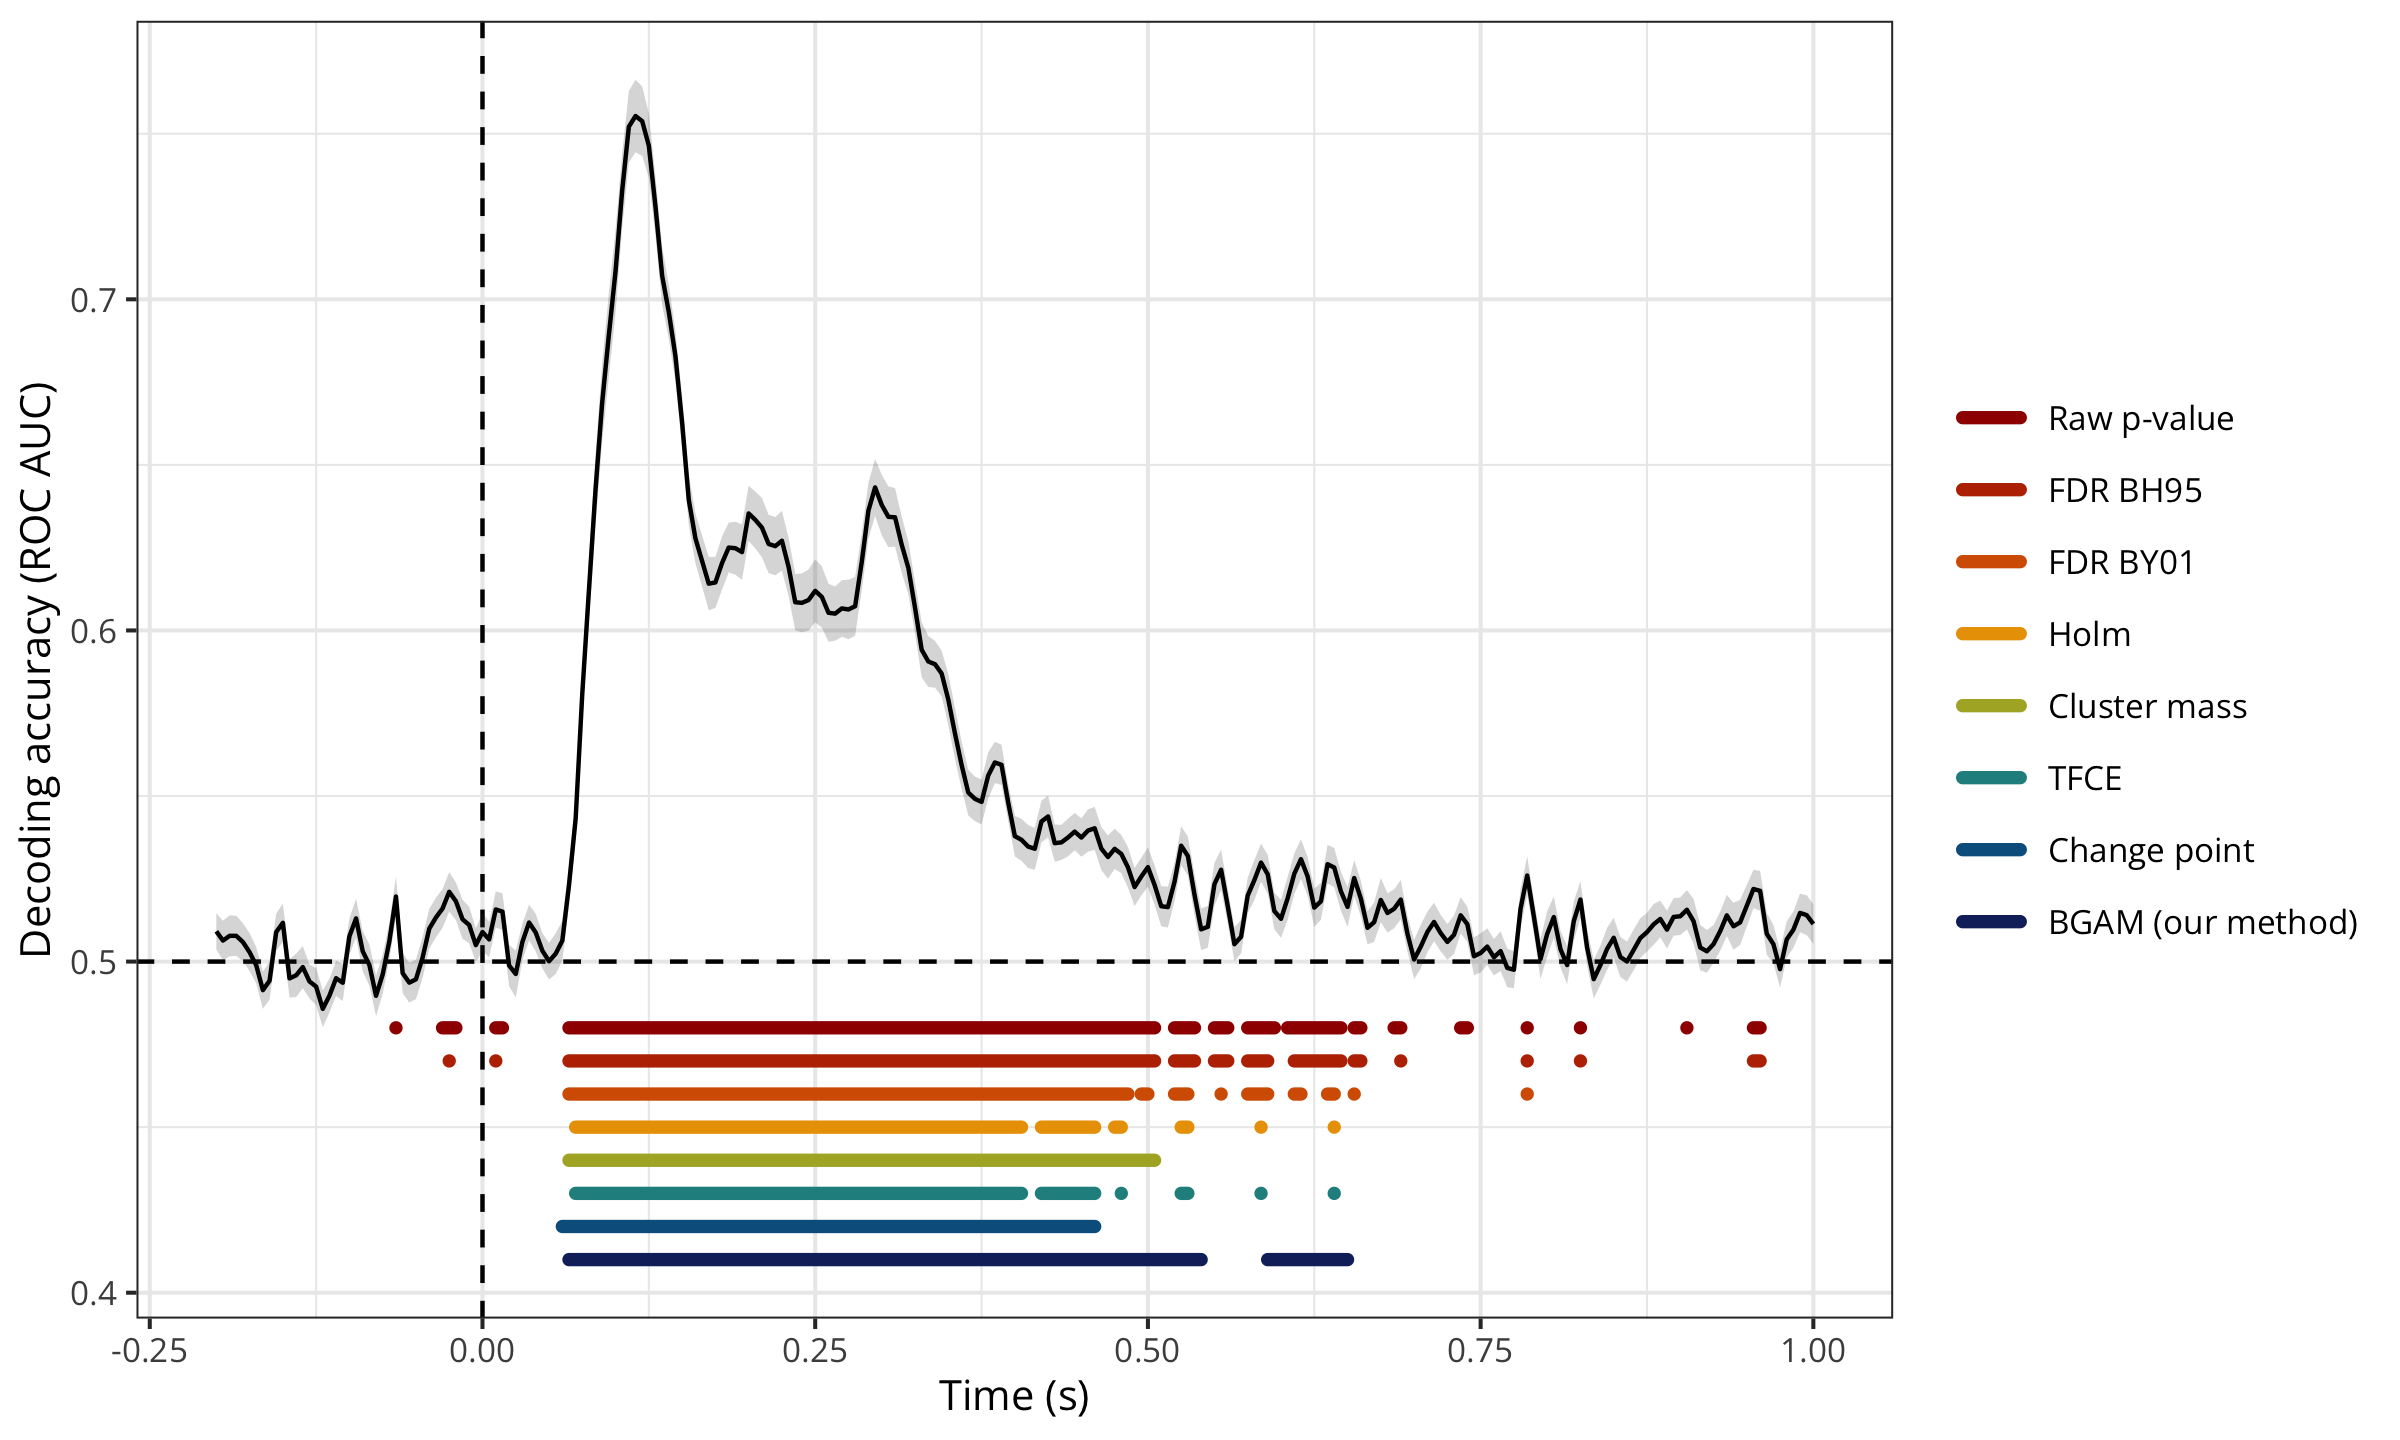
\includegraphics[width=1\textwidth,height=\textheight]{manuscript_files/figure-pdf/fig-onset-offset-1.png}

}

\end{figure}%

We then assessed the sensitivity of the various methods using a form of
permutation-based sensitivity study, which consisted of the following
steps. First, we created a large number of split halves of the data,
that is, subsets of the dataset containing only 16 out of 32
participants. For each possible pair of subsets, we have 16 possible
levels of overlap/similarity that can be quantified using the Jaccard
index, ranging from 0 (perfectly disjoints subsets) to \(\approx0.88\)
(identical subsets except one participant). For each of these 16 levels
of Jaccard similarity, we created 1,000 pairs of subsets, resulting in
16,000 pairs of subsets in total. For each of these pairs, we estimated
the onset and offset according to each method and computed the absolute
difference in onset/offset estimates. Finally, we estimated the
Spearman's rank correlation coefficient (which quantifies the strength
of a monotonic relation between two variables) between the Jaccard
similarity and the absolute difference in onset/offset estimates. The
rational for this procedure is that sensitive methods should produce
similar onset/offset estimates for similar subsets and dissimilar
onset/offset estimates for dissimilar subsets. The results of this
procedure are summarised in Figure~\ref{fig-splits-similarity}.

\begin{figure}[!htb]

\caption{\label{fig-splits-similarity}Relation between data subsets'
dissimilarity (x-axis) and difference in onset (blue) and offset
(orange) estimates (y-axis) according to each method.}

\centering{

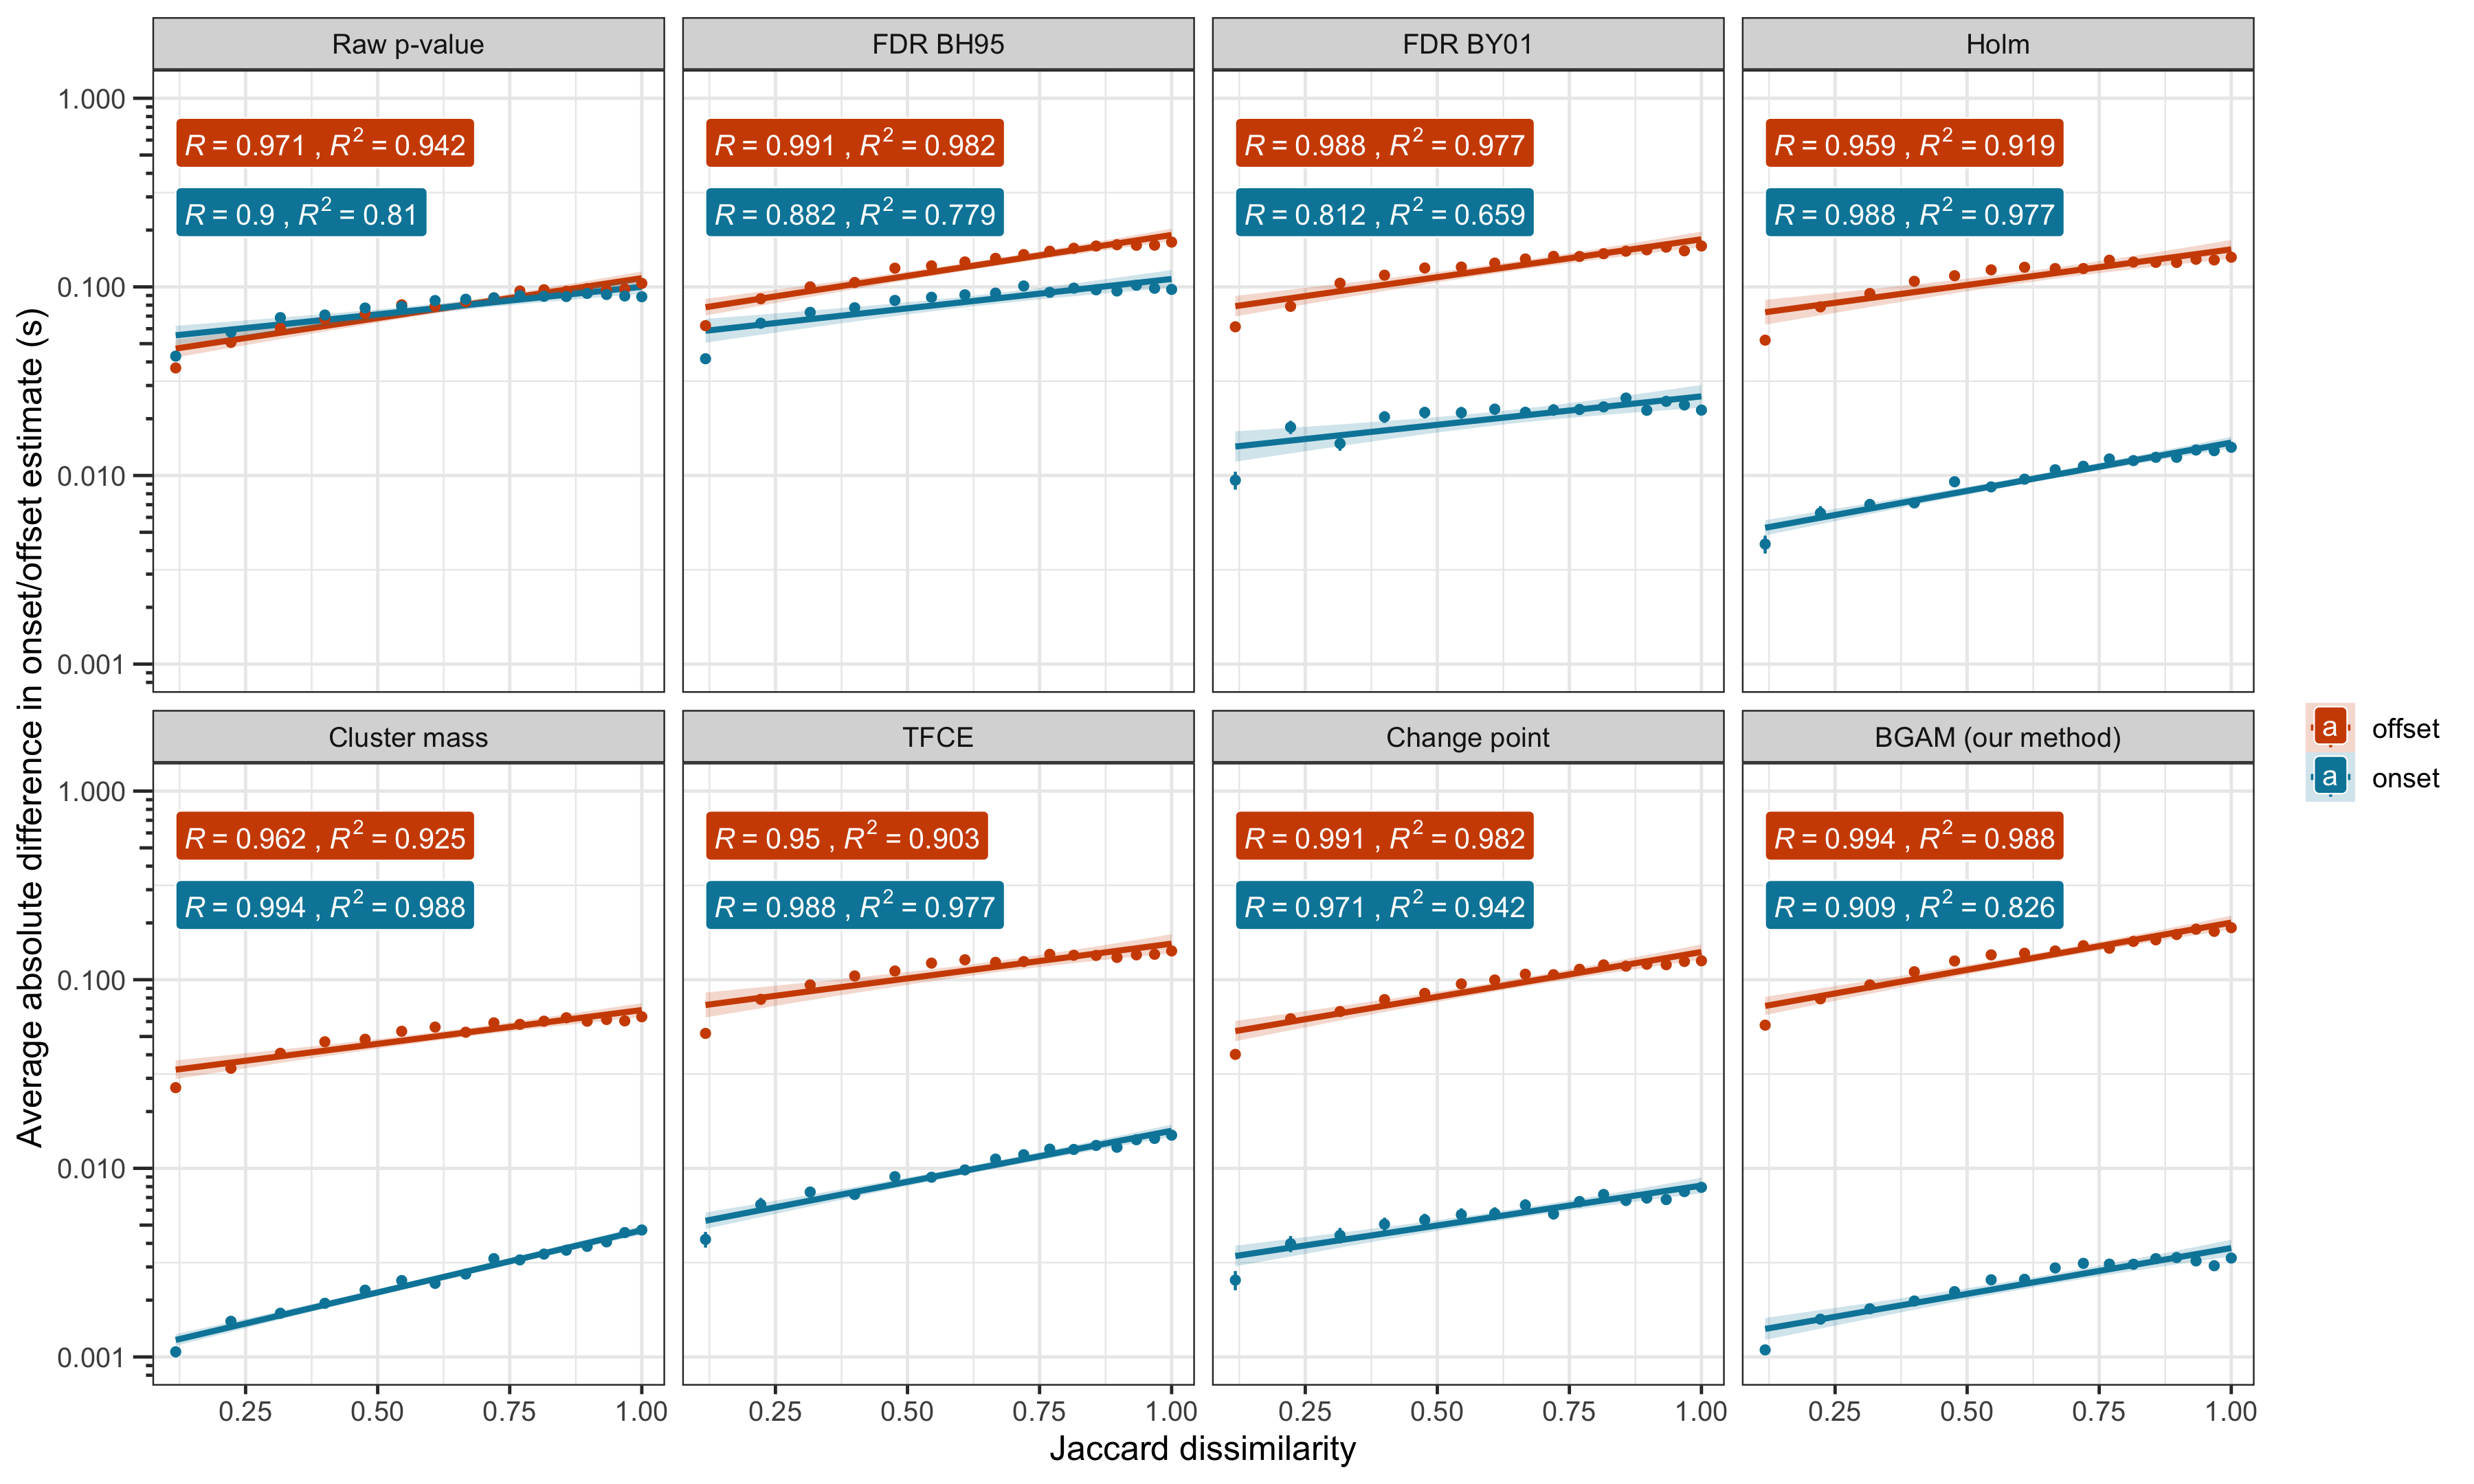
\includegraphics[width=1\textwidth,height=\textheight]{manuscript_files/figure-pdf/fig-splits-similarity-1.png}

}

\end{figure}%

This figure shows that, among the methods that performed best in the
simulation study (i.e., \texttt{Cluster\ mass}, \texttt{Change\ point},
and \texttt{BGAM}), onset estimates remain highly stable across subsets
of participants with varying Jaccard similarity, it varies from around
1ms for most similar subsets to around 10ms for most dissimilar subsets.
Additionally, for both onset and offset estimates, the average pairwise
difference increases monotonically with Jaccard dissimilarity, as
indicated by the Spearman's rank correlation coefficient. For the onset
estimates, the \texttt{Holm}, \texttt{Cluster\ mass}, \texttt{TFCE}, and
\texttt{BGAM} methods exhibit the strongest monotonic relation with
subset similarity (all \(\rho\text{s} > 0.9\)), whereas for offset
estimates, all methods demonstrate excellent performance (all
\(\rho\text{s} > 0.9\)) with the \texttt{BGAM} method showing the
highest sensitivity (\(\rho\approx0.994\)). However, given the aberrant
clusters identified by the \texttt{Raw\ p-value}, \texttt{FDR\ BH95},
and \texttt{FDR\ BY01} methods (see Figure~\ref{fig-onset-offset}),
their sensitivity to variation in subset similarity is not meaningful.

\section{Discussion}\label{discussion}

In brief, our results show that the model-based approach we introduced
outperforms conventional cluster-based methods in identifying the onset
and offset of M/EEG effects. We first assessed the performance of this
approach on simulated data allowing us to evaluate the method's ability
to recover ground-truth onset and offset values. We then assessed its
performance on actual MEG data, allowing us to assess its sensitivity to
realistic data properties (subset similarity). Together, these results
highlight desirable properties for any method aiming to precisely and
reliably estimate the onset and offset of M/EEG effects: it should i)
recover true onsets and offsets in simulation (good asymptotic
behaviour), ii) identify clusters that are interpretable and consistent
in empirical data, and iii) show sensitivity to subtle changes in the
data. Our approach meets all three of these desiderata.

As with previous simulation studies (e.g.,
\citeproc{ref-rousselet2008}{Rousselet et al., 2008};
\citeproc{ref-sassenhagen2019}{Sassenhagen \& Draschkow, 2019}), results
inevitably depend on design choices, including the specific
cluster-forming algorithm and threshold (for cluster-based methods), the
signal-to-noise ratio, and the potential degradation of temporal
resolution introduced by preprocessing steps such as low-pass filtering.
However, these constraints apply equally to all methods tested, so
relative differences in performance remain meaningful.

Interestingly, the TFCE method performed worse than the traditional
cluster-sum approach, consistent with the predictions of Rousselet
(\citeproc{ref-rousselet_using_2025}{2025}) based on the original
findings of S. Smith \& Nichols (\citeproc{ref-smith2009}{2009}). We
also found a striking overlap in the clusters identified by the
\texttt{Holm} and \texttt{TFCE} procedures (cf.
Figure~\ref{fig-onset-offset} and Figure~\ref{fig-splits-similarity}).
Whereas these two approaches are conceptually distinct; \texttt{Holm}
controlling the family-wise error rate through sequential \emph{p}-value
adjustment, \texttt{TFCE} enhancing signal based on spatiotemporal
support; their similarity in practice may arise because both effectively
prioritise extended, moderately strong effects over isolated
high-intensity points. This convergence warrants further methodological
work.

A critical requirement for any model-based approach is that the model
must adequately capture the underlying data-generating process.
Misspecified models are likely to produce biased or unreliable
onset/offset estimates. This underscores the importance of thorough
model diagnostics, including posterior predictive checks, fit
assessments, and model comparison (\citeproc{ref-gelman2020}{Gelman et
al., 2020}). An important and related methodological consideration
concerns the selection of model hyperparameters, such as the number of
basis functions and the threshold for posterior odds. Although our
simulations suggest that these parameters influence the precision and
reliability of onset and offset estimates, optimal values may vary
depending on the signal's temporal dynamics and signal-to-noise
characteristics. Future work could explore principled approaches to
hyperparameter tuning, including cross-validation or fully Bayesian
model selection using tools such as leave-one-out cross-validation
(LOO-CV) or Bayes factors (\citeproc{ref-gelman2020}{Gelman et al.,
2020}). We provide initial guidance in \hyperref[apx-basis]{Appendix~B}
and advocate for future development of adaptive heuristics to support
flexible yet parsimonious model specification.

Currently, our approach estimates temporal effects independently at each
sensor (1D temporal data). Extending the current framework to
incorporate additional temporal (see \hyperref[apx-2D]{Appendix~A}) or
spatial dimensions would improve both sensitivity and interpretability.
Such extensions could draw on methods from spatial epidemiology and
geostatistics using either GAMMs or approximate Gaussian process
regression (e.g., \citeproc{ref-rasmussen2005}{Rasmussen \& Williams,
2005}; \citeproc{ref-riutort-mayol_practical_2023}{Riutort-Mayol et al.,
2023}), depending on computational feasibility.

To facilitate adoption, we developed the \texttt{neurogram} open-source
\texttt{R} package (\citeproc{ref-neurogam}{Nalborczyk, 2025}), which
implements the proposed method using \texttt{brms}. The package
integrates seamlessly with \texttt{MNE-Python}
(\citeproc{ref-gramfort2013}{Gramfort, 2013}), enabling researchers to
process M/EEG data in \texttt{Python} and import them directly into
\texttt{R} for model-based inference without cumbersome data export.
This interoperability, described in \hyperref[apx-package]{Appendix~C},
is designed to encourage broader use of model-based approaches in
cognitive neuroscience.

In conclusion, we introduced a model-based approach for estimating the
onset and offset of M/EEG effects. Across simulated and empirical
datasets, we showed that the method yields more precise and sensitive
estimates than conventional cluster-based approaches. These results
highlight the potential of flexible, model-based alternatives for
characterising time-resolved neural dynamics, particularly in
applications where accurate temporal localisation is critical.

\newpage

\setcounter{secnumdepth}{0}

\section{Data and code availability}\label{data-and-code-availability}

The simulation results as well as the \texttt{R} code to reproduce the
simulations are available at:
\url{https://github.com/lnalborczyk/brms_meeg}. The \texttt{neurogam\ R}
package is available at \url{https://github.com/lnalborczyk/neurogam}.

\section{Packages}\label{packages}

We used R version 4.4.3 (\citeproc{ref-base}{R Core Team, 2025}) and the
following R packages: assertthat v. 0.2.1
(\citeproc{ref-assertthat}{Wickham, 2019}), brms v. 2.22.0
(\citeproc{ref-brms2017}{Bürkner, 2017}, \citeproc{ref-brms2018}{2018},
\citeproc{ref-brms2021}{2021}), doParallel v. 1.0.17
(\citeproc{ref-doParallel}{Corporation \& Weston, 2022}), foreach v.
1.5.2 (\citeproc{ref-foreach}{Microsoft \& Weston, 2022}), furrr v.
0.3.1 (\citeproc{ref-furrr}{Vaughan \& Dancho, 2022}), future v. 1.58.0
(\citeproc{ref-future}{Bengtsson, 2021}), ggpubr v. 0.6.0
(\citeproc{ref-ggpubr}{Kassambara, 2023}), ggrepel v. 0.9.6
(\citeproc{ref-ggrepel}{Slowikowski, 2024}), glue v. 1.8.0
(\citeproc{ref-glue}{Hester \& Bryan, 2024}), grateful v. 0.2.12
(\citeproc{ref-grateful}{Rodriguez-Sanchez \& Jackson, 2024}), gt v.
1.0.0 (\citeproc{ref-gt}{Iannone et al., 2025}), knitr v. 1.50
(\citeproc{ref-knitr2014}{Xie, 2014}, \citeproc{ref-knitr2015}{2015},
\citeproc{ref-knitr2025}{2025}), MetBrewer v. 0.2.0
(\citeproc{ref-MetBrewer}{Mills, 2022}), mgcv v. 1.9.3
(\citeproc{ref-mgcv2003}{Wood, 2003b}, \citeproc{ref-mgcv2004}{2004},
\citeproc{ref-mgcv2011}{2011}, \citeproc{ref-mgcv2017}{2017c};
\citeproc{ref-mgcv2016}{Wood et al., 2016}), neurogam v. 0.0.1
(\citeproc{ref-neurogam}{Nalborczyk, 2025}), pakret v. 0.2.2
(\citeproc{ref-pakret}{Gallou, 2024}), patchwork v. 1.3.0
(\citeproc{ref-patchwork}{T. L. Pedersen, 2024}), rmarkdown v. 2.29
(\citeproc{ref-rmarkdown2024}{Allaire et al., 2024};
\citeproc{ref-rmarkdown2018}{Xie et al., 2018},
\citeproc{ref-rmarkdown2020}{2020}), scales v. 1.4.0
(\citeproc{ref-scales}{Wickham et al., 2025}), scico v. 1.5.0
(\citeproc{ref-scico}{T. L. Pedersen \& Crameri, 2023}), signal v. 1.8.1
(\citeproc{ref-signal}{signal developers, 2023}), tictoc v. 1.2.1
(\citeproc{ref-tictoc}{Izrailev, 2024}), tidybayes v. 3.0.7
(\citeproc{ref-tidybayes}{Kay, 2024}), tidytext v. 0.4.2
(\citeproc{ref-tidytext}{Silge \& Robinson, 2016}), tidyverse v. 2.0.0
(\citeproc{ref-tidyverse}{Wickham et al., 2019}).

\section{Acknolwedgements}\label{acknolwedgements}

Centre de Calcul Intensif d'Aix-Marseille is acknowledged for granting
access to its high performance computing resources.

\newpage

\section{References}\label{references}

\phantomsection\label{refs}
\begin{CSLReferences}{1}{0}
\bibitem[\citeproctext]{ref-abugaber2023}
Abugaber, D., Finestrat, I., Luque, A., \& Morgan-Short, K. (2023).
Generalized additive mixed modeling of EEG supports dual-route accounts
of morphosyntax in suggesting no word frequency effects on processing of
regular grammatical forms. \emph{Journal of Neurolinguistics},
\emph{67}, 101137.
\url{https://doi.org/10.1016/j.jneuroling.2023.101137}

\bibitem[\citeproctext]{ref-rmarkdown2024}
Allaire, J., Xie, Y., Dervieux, C., McPherson, J., Luraschi, J., Ushey,
K., Atkins, A., Wickham, H., Cheng, J., Chang, W., \& Iannone, R.
(2024). \emph{{rmarkdown}: Dynamic documents for r}.
\url{https://github.com/rstudio/rmarkdown}

\bibitem[\citeproctext]{ref-baayen2020}
Baayen, R. H., \& Linke, M. (2020). \emph{Generalized Additive Mixed
Models} (pp. 563--591). Springer International Publishing.
\url{https://doi.org/10.1007/978-3-030-46216-1_23}

\bibitem[\citeproctext]{ref-baayen2018}
Baayen, R. H., Rij, J. van, Cat, C. de, \& Wood, S. (2018).
\emph{Autocorrelated errors in experimental data in the language
sciences: Some solutions offered by generalized additive mixed models}
(pp. 49--69). Springer International Publishing.
\url{https://doi.org/10.1007/978-3-319-69830-4_4}

\bibitem[\citeproctext]{ref-future}
Bengtsson, H. (2021). A unifying framework for parallel and distributed
processing in r using futures. \emph{The R Journal}, \emph{13}(2),
208--227. \url{https://doi.org/10.32614/RJ-2021-048}

\bibitem[\citeproctext]{ref-benjamini1995}
Benjamini, Y., \& Hochberg, Y. (1995). Controlling the False Discovery
Rate: A Practical and Powerful Approach to Multiple Testing.
\emph{Journal of the Royal Statistical Society Series B: Statistical
Methodology}, \emph{57}(1), 289--300.
\url{https://doi.org/10.1111/j.2517-6161.1995.tb02031.x}

\bibitem[\citeproctext]{ref-benjamini2001}
Benjamini, Y., \& Yekutieli, D. (2001). The control of the false
discovery rate in multiple testing under dependency. \emph{The Annals of
Statistics}, \emph{29}(4). \url{https://doi.org/10.1214/aos/1013699998}

\bibitem[\citeproctext]{ref-bullmore1999}
Bullmore, E. T., Suckling, J., Overmeyer, S., Rabe-Hesketh, S., Taylor,
E., \& Brammer, M. J. (1999). Global, voxel, and cluster tests, by
theory and permutation, for a difference between two groups of
structural MR images of the brain. \emph{IEEE Transactions on Medical
Imaging}, \emph{18}(1), 32--42. \url{https://doi.org/10.1109/42.750253}

\bibitem[\citeproctext]{ref-brms2017}
Bürkner, P.-C. (2017). {brms}: An {R} package for {Bayesian} multilevel
models using {Stan}. \emph{Journal of Statistical Software},
\emph{80}(1), 1--28. \url{https://doi.org/10.18637/jss.v080.i01}

\bibitem[\citeproctext]{ref-brms2018}
Bürkner, P.-C. (2018). Advanced {Bayesian} multilevel modeling with the
{R} package {brms}. \emph{The R Journal}, \emph{10}(1), 395--411.
\url{https://doi.org/10.32614/RJ-2018-017}

\bibitem[\citeproctext]{ref-brms2021}
Bürkner, P.-C. (2021). Bayesian item response modeling in {R} with
{brms} and {Stan}. \emph{Journal of Statistical Software},
\emph{100}(5), 1--54. \url{https://doi.org/10.18637/jss.v100.i05}

\bibitem[\citeproctext]{ref-doParallel}
Corporation, M., \& Weston, S. (2022). \emph{{doParallel}: Foreach
parallel adaptor for the {``{parallel}''} package}.
\url{https://CRAN.R-project.org/package=doParallel}

\bibitem[\citeproctext]{ref-delorme2004}
Delorme, A., \& Makeig, S. (2004). EEGLAB: an open source toolbox for
analysis of single-trial EEG dynamics including independent component
analysis. \emph{Journal of Neuroscience Methods}, \emph{134}(1), 9--21.
\url{https://doi.org/10.1016/j.jneumeth.2003.10.009}

\bibitem[\citeproctext]{ref-dinga2021}
Dinga, R., Fraza, C. J., Bayer, J. M. M., Kia, S. M., Beckmann, C. F.,
\& Marquand, A. F. (2021). \emph{Normative modeling of neuroimaging data
using generalized additive models of location scale and shape}.
\url{http://dx.doi.org/10.1101/2021.06.14.448106}

\bibitem[\citeproctext]{ref-dunagan2025}
Dunagan, D., Jordan, T., Hale, J. T., Pylkkänen, L., \& Chacón, D. A.
(2025). Evaluating the timecourses of morpho-orthographic, lexical, and
grammatical processing following rapid parallel visual presentation: An
EEG investigation in English. \emph{Cognition}, \emph{257}, 106080.
\url{https://doi.org/10.1016/j.cognition.2025.106080}

\bibitem[\citeproctext]{ref-dunn1961}
Dunn, O. J. (1961). Multiple Comparisons among Means. \emph{Journal of
the American Statistical Association}, \emph{56}(293), 52--64.
\url{https://doi.org/10.1080/01621459.1961.10482090}

\bibitem[\citeproctext]{ref-ehinger_unfold_2019}
Ehinger, B. V., \& Dimigen, O. (2019). Unfold: An integrated toolbox for
overlap correction, non-linear modeling, and regression-based {EEG}
analysis. \emph{PeerJ}, \emph{7}, e7838.
\url{https://doi.org/10.7717/peerj.7838}

\bibitem[\citeproctext]{ref-frossard2022}
Frossard, J., \& Renaud, O. (2022). The cluster depth tests: Toward
point-wise strong control of the family-wise error rate in massively
univariate tests with application to M/EEG. \emph{NeuroImage},
\emph{247}, 118824.
\url{https://doi.org/10.1016/j.neuroimage.2021.118824}

\bibitem[\citeproctext]{ref-gabry2019}
Gabry, J., Simpson, D., Vehtari, A., Betancourt, M., \& Gelman, A.
(2019). Visualization in Bayesian work{fl}ow. \emph{Journal of the Royal
Statistical Society: Series A (Statistics in Society)}, \emph{182}(2),
389--402. \url{https://doi.org/10.1111/rssa.12378}

\bibitem[\citeproctext]{ref-pakret}
Gallou, A. (2024). \emph{{pakret}: Cite {``{R}''} packages on the fly in
{``{R Markdown}''} and {``{Quarto}''}}.
\url{https://CRAN.R-project.org/package=pakret}

\bibitem[\citeproctext]{ref-gelman2020}
Gelman, A., Vehtari, A., Simpson, D., Margossian, C. C., Carpenter, B.,
Yao, Y., Kennedy, L., Gabry, J., Bürkner, P.-C., \& Modrák, M. (2020).
Bayesian workflow. \emph{arXiv:2011.01808 {[}Stat{]}}.
\url{http://arxiv.org/abs/2011.01808}

\bibitem[\citeproctext]{ref-gramfort2013}
Gramfort, A. (2013). MEG and EEG data analysis with MNE-python.
\emph{Frontiers in Neuroscience}, \emph{7}.
\url{https://doi.org/10.3389/fnins.2013.00267}

\bibitem[\citeproctext]{ref-hastie2017}
Hastie, T. J., \& Tibshirani, R. J. (2017). \emph{Generalized Additive
Models}. Routledge. \url{https://doi.org/10.1201/9780203753781}

\bibitem[\citeproctext]{ref-glue}
Hester, J., \& Bryan, J. (2024). \emph{{glue}: Interpreted string
literals}. \url{https://CRAN.R-project.org/package=glue}

\bibitem[\citeproctext]{ref-holm1979}
Holm, S. (1979). A simple sequentially rejective multiple test
procedure. \emph{Scandinavian Journal of Statistics}, \emph{6}(2),
65--70. \url{http://www.jstor.org/stable/4615733}

\bibitem[\citeproctext]{ref-gt}
Iannone, R., Cheng, J., Schloerke, B., Hughes, E., Lauer, A., Seo, J.,
Brevoort, K., \& Roy, O. (2025). \emph{{gt}: Easily create
presentation-ready display tables}.
\url{https://CRAN.R-project.org/package=gt}

\bibitem[\citeproctext]{ref-tictoc}
Izrailev, S. (2024). \emph{{tictoc}: Functions for timing r scripts, as
well as implementations of {``{Stack}''} and {``{StackList}''}
structures}. \url{https://CRAN.R-project.org/package=tictoc}

\bibitem[\citeproctext]{ref-ggpubr}
Kassambara, A. (2023). \emph{{ggpubr}: {``{ggplot2}''} based publication
ready plots}. \url{https://CRAN.R-project.org/package=ggpubr}

\bibitem[\citeproctext]{ref-tidybayes}
Kay, M. (2024). \emph{{tidybayes}: Tidy data and geoms for {Bayesian}
models}. \url{https://doi.org/10.5281/zenodo.1308151}

\bibitem[\citeproctext]{ref-changepoint}
Killick, R., Haynes, K., \& Eckley, I. A. (2022). \emph{{changepoint}:
An {R} package for changepoint analysis}.
\url{https://CRAN.R-project.org/package=changepoint}

\bibitem[\citeproctext]{ref-king2014}
King, J.-R., \& Dehaene, S. (2014). Characterizing the dynamics of
mental representations: the temporal generalization method. \emph{Trends
in Cognitive Sciences}, \emph{18}(4), 203--210.
\url{https://doi.org/10.1016/j.tics.2014.01.002}

\bibitem[\citeproctext]{ref-kruschke2017}
Kruschke, J. K., \& Liddell, T. M. (2017). The Bayesian New Statistics:
Hypothesis testing, estimation, meta-analysis, and power analysis from a
Bayesian perspective. \emph{Psychonomic Bulletin \& Review},
\emph{25}(1), 178--206. \url{https://doi.org/10.3758/s13423-016-1221-4}

\bibitem[\citeproctext]{ref-maris2011}
Maris, E. (2011). Statistical testing in electrophysiological studies.
\emph{Psychophysiology}, \emph{49}(4), 549--565.
\url{https://doi.org/10.1111/j.1469-8986.2011.01320.x}

\bibitem[\citeproctext]{ref-maris2007}
Maris, E., \& Oostenveld, R. (2007). Nonparametric statistical testing
of EEG- and MEG-data. \emph{Journal of Neuroscience Methods},
\emph{164}(1), 177--190.
\url{https://doi.org/10.1016/j.jneumeth.2007.03.024}

\bibitem[\citeproctext]{ref-meulman2023}
Meulman, N., Sprenger, S. A., Schmid, M. S., \& Wieling, M. (2023).
GAM-based individual difference measures for L2 ERP studies.
\emph{Research Methods in Applied Linguistics}, \emph{2}(3), 100079.
\url{https://doi.org/10.1016/j.rmal.2023.100079}

\bibitem[\citeproctext]{ref-meulman2015}
Meulman, N., Wieling, M., Sprenger, S. A., Stowe, L. A., \& Schmid, M.
S. (2015). Age Effects in L2 Grammar Processing as Revealed by ERPs and
How (Not) to Study Them. \emph{PLOS ONE}, \emph{10}(12), e0143328.
\url{https://doi.org/10.1371/journal.pone.0143328}

\bibitem[\citeproctext]{ref-foreach}
Microsoft, \& Weston, S. (2022). \emph{{foreach}: Provides foreach
looping construct}. \url{https://CRAN.R-project.org/package=foreach}

\bibitem[\citeproctext]{ref-miller2025}
Miller, D. L. (2025). Bayesian views of generalized additive modelling.
\emph{Methods in Ecology and Evolution}.
\url{https://doi.org/10.1111/2041-210x.14498}

\bibitem[\citeproctext]{ref-MetBrewer}
Mills, B. R. (2022). \emph{{MetBrewer}: Color palettes inspired by works
at the metropolitan museum of art}.
\url{https://CRAN.R-project.org/package=MetBrewer}

\bibitem[\citeproctext]{ref-neurogam}
Nalborczyk, L. (2025). \emph{{neurogam}: Precise temporal localisation
of m/EEG effects with bayesian generalised additive multilevel models}.
\url{https://github.com/lnalborczyk/neurogam}

\bibitem[\citeproctext]{ref-nalborczyk2019}
Nalborczyk, L., Batailler, C., Lœvenbruck, H., Vilain, A., \& Bürkner,
P.-C. (2019). An Introduction to Bayesian Multilevel Models Using brms:
A Case Study of Gender Effects on Vowel Variability in Standard
Indonesian. \emph{Journal of Speech, Language, and Hearing Research},
\emph{62}(5), 1225--1242.
\url{https://doi.org/10.1044/2018_jslhr-s-18-0006}

\bibitem[\citeproctext]{ref-nalborczyk:inprep}
Nalborczyk, L., Hauw, F., Torcy, H. de, Dehaene, S., \& Cohen, L. (in
preparation). \emph{Neural and representational dynamics of tickertape
synesthesia}.

\bibitem[\citeproctext]{ref-pedersen_hierarchical_2019}
Pedersen, E. J., Miller, D. L., Simpson, G. L., \& Ross, N. (2019).
Hierarchical generalized additive models in ecology: An introduction
with mgcv. \emph{PeerJ}, \emph{7}, e6876.
\url{https://doi.org/10.7717/peerj.6876}

\bibitem[\citeproctext]{ref-patchwork}
Pedersen, T. L. (2024). \emph{{patchwork}: The composer of plots}.
\url{https://CRAN.R-project.org/package=patchwork}

\bibitem[\citeproctext]{ref-scico}
Pedersen, T. L., \& Crameri, F. (2023). \emph{{scico}: Colour palettes
based on the scientific colour-maps}.
\url{https://CRAN.R-project.org/package=scico}

\bibitem[\citeproctext]{ref-pernet2011}
Pernet, C. R., Chauveau, N., Gaspar, C., \& Rousselet, G. A. (2011).
LIMO EEG: A Toolbox for Hierarchical LInear MOdeling of
ElectroEncephaloGraphic Data. \emph{Computational Intelligence and
Neuroscience}, \emph{2011}, 1--11.
\url{https://doi.org/10.1155/2011/831409}

\bibitem[\citeproctext]{ref-pernet2015}
Pernet, C. R., Latinus, M., Nichols, T. E., \& Rousselet, G. A. (2015).
Cluster-based computational methods for mass univariate analyses of
event-related brain potentials/fields: A simulation study. \emph{Journal
of Neuroscience Methods}, \emph{250}, 85--93.
\url{https://doi.org/10.1016/j.jneumeth.2014.08.003}

\bibitem[\citeproctext]{ref-base}
R Core Team. (2025). \emph{{R}: A language and environment for
statistical computing}. R Foundation for Statistical Computing.
\url{https://www.R-project.org/}

\bibitem[\citeproctext]{ref-rasmussen2005}
Rasmussen, C. E., \& Williams, C. K. I. (2005). \emph{Gaussian Processes
for Machine Learning}.
\url{https://doi.org/10.7551/mitpress/3206.001.0001}

\bibitem[\citeproctext]{ref-rigby2005}
Rigby, R. A., \& Stasinopoulos, D. M. (2005). Generalized Additive
Models for Location, Scale and Shape. \emph{Journal of the Royal
Statistical Society Series C: Applied Statistics}, \emph{54}(3),
507--554. \url{https://doi.org/10.1111/j.1467-9876.2005.00510.x}

\bibitem[\citeproctext]{ref-vanrij2019}
Rij, J. van, Hendriks, P., Rijn, H. van, Baayen, R. H., \& Wood, S. N.
(2019). Analyzing the Time Course of Pupillometric Data. \emph{Trends in
Hearing}, \emph{23}. \url{https://doi.org/10.1177/2331216519832483}

\bibitem[\citeproctext]{ref-riutort-mayol_practical_2023}
Riutort-Mayol, G., Bürkner, P.-C., Andersen, M. R., Solin, A., \&
Vehtari, A. (2023). Practical {Hilbert} space approximate {Bayesian
Gaussian} processes for probabilistic programming. \emph{Statistics and
Computing}, \emph{33}(1), 17.
\url{https://doi.org/10.1007/s11222-022-10167-2}

\bibitem[\citeproctext]{ref-grateful}
Rodriguez-Sanchez, F., \& Jackson, C. P. (2024). \emph{{grateful}:
Facilitate citation of {R} packages}.
\url{https://pakillo.github.io/grateful/}

\bibitem[\citeproctext]{ref-rosenblatt2018}
Rosenblatt, J. D., Finos, L., Weeda, W. D., Solari, A., \& Goeman, J. J.
(2018). All-Resolutions Inference for brain imaging. \emph{NeuroImage},
\emph{181}, 786--796.
\url{https://doi.org/10.1016/j.neuroimage.2018.07.060}

\bibitem[\citeproctext]{ref-rousselet_using_2025}
Rousselet, G. A. (2025). Using cluster-based permutation tests to
estimate {MEG}/{EEG} onsets: {How} bad is it? \emph{European Journal of
Neuroscience}, \emph{61}(1), e16618.
\url{https://doi.org/10.1111/ejn.16618}

\bibitem[\citeproctext]{ref-rousselet2008}
Rousselet, G. A., Pernet, C. R., Bennett, P. J., \& Sekuler, A. B.
(2008). Parametric study of EEG sensitivity to phase noise during face
processing. \emph{BMC Neuroscience}, \emph{9}(1).
\url{https://doi.org/10.1186/1471-2202-9-98}

\bibitem[\citeproctext]{ref-sassenhagen2019}
Sassenhagen, J., \& Draschkow, D. (2019). Cluster{-}based permutation
tests of MEG/EEG data do not establish significance of effect latency or
location. \emph{Psychophysiology}, \emph{56}(6).
\url{https://doi.org/10.1111/psyp.13335}

\bibitem[\citeproctext]{ref-signal}
signal developers. (2023). \emph{{signal}: Signal processing}.
\url{https://r-forge.r-project.org/projects/signal/}

\bibitem[\citeproctext]{ref-tidytext}
Silge, J., \& Robinson, D. (2016). {tidytext}: Text mining and analysis
using tidy data principles in r. \emph{JOSS}, \emph{1}(3).
\url{https://doi.org/10.21105/joss.00037}

\bibitem[\citeproctext]{ref-skukies_modelling_2021}
Skukies, R., \& Ehinger, B. (2021). Modelling event duration and overlap
during {EEG} analysis. \emph{Journal of Vision}, \emph{21}(9), 2037.
\url{https://doi.org/10.1167/jov.21.9.2037}

\bibitem[\citeproctext]{ref-skukies_brain_2024}
Skukies, R., Schepers, J., \& Ehinger, B. (2024, December 9).
\emph{Brain responses vary in duration - modeling strategies and
challenges}. \url{https://doi.org/10.1101/2024.12.05.626938}

\bibitem[\citeproctext]{ref-ggrepel}
Slowikowski, K. (2024). \emph{{ggrepel}: Automatically position
non-overlapping text labels with {``{ggplot2}''}}.
\url{https://CRAN.R-project.org/package=ggrepel}

\bibitem[\citeproctext]{ref-smith2014a}
Smith, N. J., \& Kutas, M. (2014a). Regression{-}based estimation of ERP
waveforms: I. The rERP framework. \emph{Psychophysiology}, \emph{52}(2),
157--168. \url{https://doi.org/10.1111/psyp.12317}

\bibitem[\citeproctext]{ref-smith2014b}
Smith, N. J., \& Kutas, M. (2014b). Regression{-}based estimation of ERP
waveforms: II. Nonlinear effects, overlap correction, and practical
considerations. \emph{Psychophysiology}, \emph{52}(2), 169--181.
\url{https://doi.org/10.1111/psyp.12320}

\bibitem[\citeproctext]{ref-smith2009}
Smith, S., \& Nichols, T. (2009). Threshold-free cluster enhancement:
Addressing problems of smoothing, threshold dependence and localisation
in cluster inference. \emph{NeuroImage}, \emph{44}(1), 83--98.
\url{https://doi.org/10.1016/j.neuroimage.2008.03.061}

\bibitem[\citeproctext]{ref-suxf3skuthy2021}
Sóskuthy, M. (2021). Evaluating generalised additive mixed modelling
strategies for dynamic speech analysis. \emph{Journal of Phonetics},
\emph{84}, 101017. \url{https://doi.org/10.1016/j.wocn.2020.101017}

\bibitem[\citeproctext]{ref-tremblay2014}
Tremblay, A., \& Newman, A. J. (2014). Modeling nonlinear relationships
in ERP data using mixed{-}effects regression with R examples.
\emph{Psychophysiology}, \emph{52}(1), 124--139.
\url{https://doi.org/10.1111/psyp.12299}

\bibitem[\citeproctext]{ref-umlauf2018}
Umlauf, N., Klein, N., \& Zeileis, A. (2018). BAMLSS: Bayesian Additive
Models for Location, Scale, and Shape (and Beyond). \emph{Journal of
Computational and Graphical Statistics}, \emph{27}(3), 612--627.
\url{https://doi.org/10.1080/10618600.2017.1407325}

\bibitem[\citeproctext]{ref-reticulate}
Ushey, K., Allaire, J., \& Tang, Y. (2024). \emph{Reticulate: Interface
to 'python'}. \url{https://CRAN.R-project.org/package=reticulate}

\bibitem[\citeproctext]{ref-furrr}
Vaughan, D., \& Dancho, M. (2022). \emph{{furrr}: Apply mapping
functions in parallel using futures}.
\url{https://CRAN.R-project.org/package=furrr}

\bibitem[\citeproctext]{ref-vehtari2021}
Vehtari, A., Gelman, A., Simpson, D., Carpenter, B., \& Bürkner, P.-C.
(2021). Rank-normalization, folding, and localization: An improved Rˆ
for assessing convergence of MCMC (with discussion). \emph{Bayesian
Analysis}, \emph{16}(2). \url{https://doi.org/10.1214/20-ba1221}

\bibitem[\citeproctext]{ref-assertthat}
Wickham, H. (2019). \emph{{assertthat}: Easy pre and post assertions}.
\url{https://CRAN.R-project.org/package=assertthat}

\bibitem[\citeproctext]{ref-tidyverse}
Wickham, H., Averick, M., Bryan, J., Chang, W., McGowan, L. D.,
François, R., Grolemund, G., Hayes, A., Henry, L., Hester, J., Kuhn, M.,
Pedersen, T. L., Miller, E., Bache, S. M., Müller, K., Ooms, J.,
Robinson, D., Seidel, D. P., Spinu, V., \ldots{} Yutani, H. (2019).
Welcome to the {tidyverse}. \emph{Journal of Open Source Software},
\emph{4}(43), 1686. \url{https://doi.org/10.21105/joss.01686}

\bibitem[\citeproctext]{ref-scales}
Wickham, H., Pedersen, T. L., \& Seidel, D. (2025). \emph{{scales}:
Scale functions for visualization}.
\url{https://CRAN.R-project.org/package=scales}

\bibitem[\citeproctext]{ref-wieling2018}
Wieling, M. (2018). Analyzing dynamic phonetic data using generalized
additive mixed modeling: A tutorial focusing on articulatory differences
between L1 and L2 speakers of English. \emph{Journal of Phonetics},
\emph{70}, 86--116. \url{https://doi.org/10.1016/j.wocn.2018.03.002}

\bibitem[\citeproctext]{ref-wood2003}
Wood, S. N. (2003a). Thin Plate Regression Splines. \emph{Journal of the
Royal Statistical Society Series B: Statistical Methodology},
\emph{65}(1), 95--114. \url{https://doi.org/10.1111/1467-9868.00374}

\bibitem[\citeproctext]{ref-mgcv2003}
Wood, S. N. (2003b). Thin-plate regression splines. \emph{Journal of the
Royal Statistical Society (B)}, \emph{65}(1), 95--114.
\url{https://doi.org/10.1111/1467-9868.00374}

\bibitem[\citeproctext]{ref-mgcv2004}
Wood, S. N. (2004). Stable and efficient multiple smoothing parameter
estimation for generalized additive models. \emph{Journal of the
American Statistical Association}, \emph{99}(467), 673--686.
\url{https://doi.org/10.1198/016214504000000980}

\bibitem[\citeproctext]{ref-mgcv2011}
Wood, S. N. (2011). Fast stable restricted maximum likelihood and
marginal likelihood estimation of semiparametric generalized linear
models. \emph{Journal of the Royal Statistical Society (B)},
\emph{73}(1), 3--36.
\url{https://doi.org/10.1111/j.1467-9868.2010.00749.x}

\bibitem[\citeproctext]{ref-wood2017}
Wood, S. N. (2017a). \emph{Generalized Additive Models}. Chapman;
Hall/CRC. \url{https://doi.org/10.1201/9781315370279}

\bibitem[\citeproctext]{ref-mgcv}
Wood, S. N. (2017b). \emph{Generalized additive models: An introduction
with r} (2nd ed.). Chapman; Hall/CRC.

\bibitem[\citeproctext]{ref-mgcv2017}
Wood, S. N. (2017c). \emph{Generalized {A}dditive {M}odels: An
introduction with {R}} (2nd ed.). Chapman; Hall/CRC.

\bibitem[\citeproctext]{ref-mgcv2016}
Wood, S. N., Pya, N., \& Säfken, B. (2016). Smoothing parameter and
model selection for general smooth models (with discussion).
\emph{Journal of the American Statistical Association}, \emph{111},
1548--1575. \url{https://doi.org/10.1080/01621459.2016.1180986}

\bibitem[\citeproctext]{ref-wuxfcllhorst2025}
Wüllhorst, V., Wüllhorst, R., Overmeyer, R., \& Endrass, T. (2025).
Comprehensive Analysis of Event{-}Related Potentials of Response
Inhibition: The Role of Negative Urgency and Compulsivity.
\emph{Psychophysiology}, \emph{62}(2).
\url{https://doi.org/10.1111/psyp.70000}

\bibitem[\citeproctext]{ref-knitr2014}
Xie, Y. (2014). {knitr}: A comprehensive tool for reproducible research
in {R}. In V. Stodden, F. Leisch, \& R. D. Peng (Eds.),
\emph{Implementing reproducible computational research}. Chapman;
Hall/CRC.

\bibitem[\citeproctext]{ref-knitr2015}
Xie, Y. (2015). \emph{Dynamic documents with {R} and knitr} (2nd ed.).
Chapman; Hall/CRC. \url{https://yihui.org/knitr/}

\bibitem[\citeproctext]{ref-knitr2025}
Xie, Y. (2025). \emph{{knitr}: A general-purpose package for dynamic
report generation in {R}}. \url{https://yihui.org/knitr/}

\bibitem[\citeproctext]{ref-rmarkdown2018}
Xie, Y., Allaire, J. J., \& Grolemund, G. (2018). \emph{R markdown: The
definitive guide}. Chapman; Hall/CRC.
\url{https://bookdown.org/yihui/rmarkdown}

\bibitem[\citeproctext]{ref-rmarkdown2020}
Xie, Y., Dervieux, C., \& Riederer, E. (2020). \emph{R markdown
cookbook}. Chapman; Hall/CRC.
\url{https://bookdown.org/yihui/rmarkdown-cookbook}

\bibitem[\citeproctext]{ref-yeung2004}
Yeung, N., Bogacz, R., Holroyd, C. B., \& Cohen, J. D. (2004). Detection
of synchronized oscillations in the electroencephalogram: An evaluation
of methods. \emph{Psychophysiology}, \emph{41}(6), 822--832.
\url{https://doi.org/10.1111/j.1469-8986.2004.00239.x}

\end{CSLReferences}

\newpage

\appendix

\section{Application to 2D time-resolved decoding results
(cross-temporal generalisation)}\label{apx-2D}

\setlength{\parindent}{0pt}
\setlength{\parskip}{6pt}

We conducted a cross-temporal generalisation analysis of the decoding
data from Nalborczyk et al. (\citeproc{ref-nalborczyk:inprep}{in
preparation}), in which we assessed the performance of classifiers
trained and tested at various timesteps of the trial
(\citeproc{ref-king2014}{King \& Dehaene, 2014}). This analysis was
performed at the participant level, resulting in a 2D matrix where each
element contains the decoding accuracy (ROC AUC) of a classifier trained
at timestep \(\text{training}_{i}\) and tested at timestep
\(\text{testing}_{j}\) for each participant (Figure~\ref{fig-timegen}).

\begin{figure}[!htb]

\caption{\label{fig-timegen}Group-level average cross-temporal
generalisation matrix of decoding performance (data from
\citeproc{ref-nalborczyk:inprep}{Nalborczyk et al., in preparation}).}

\centering{

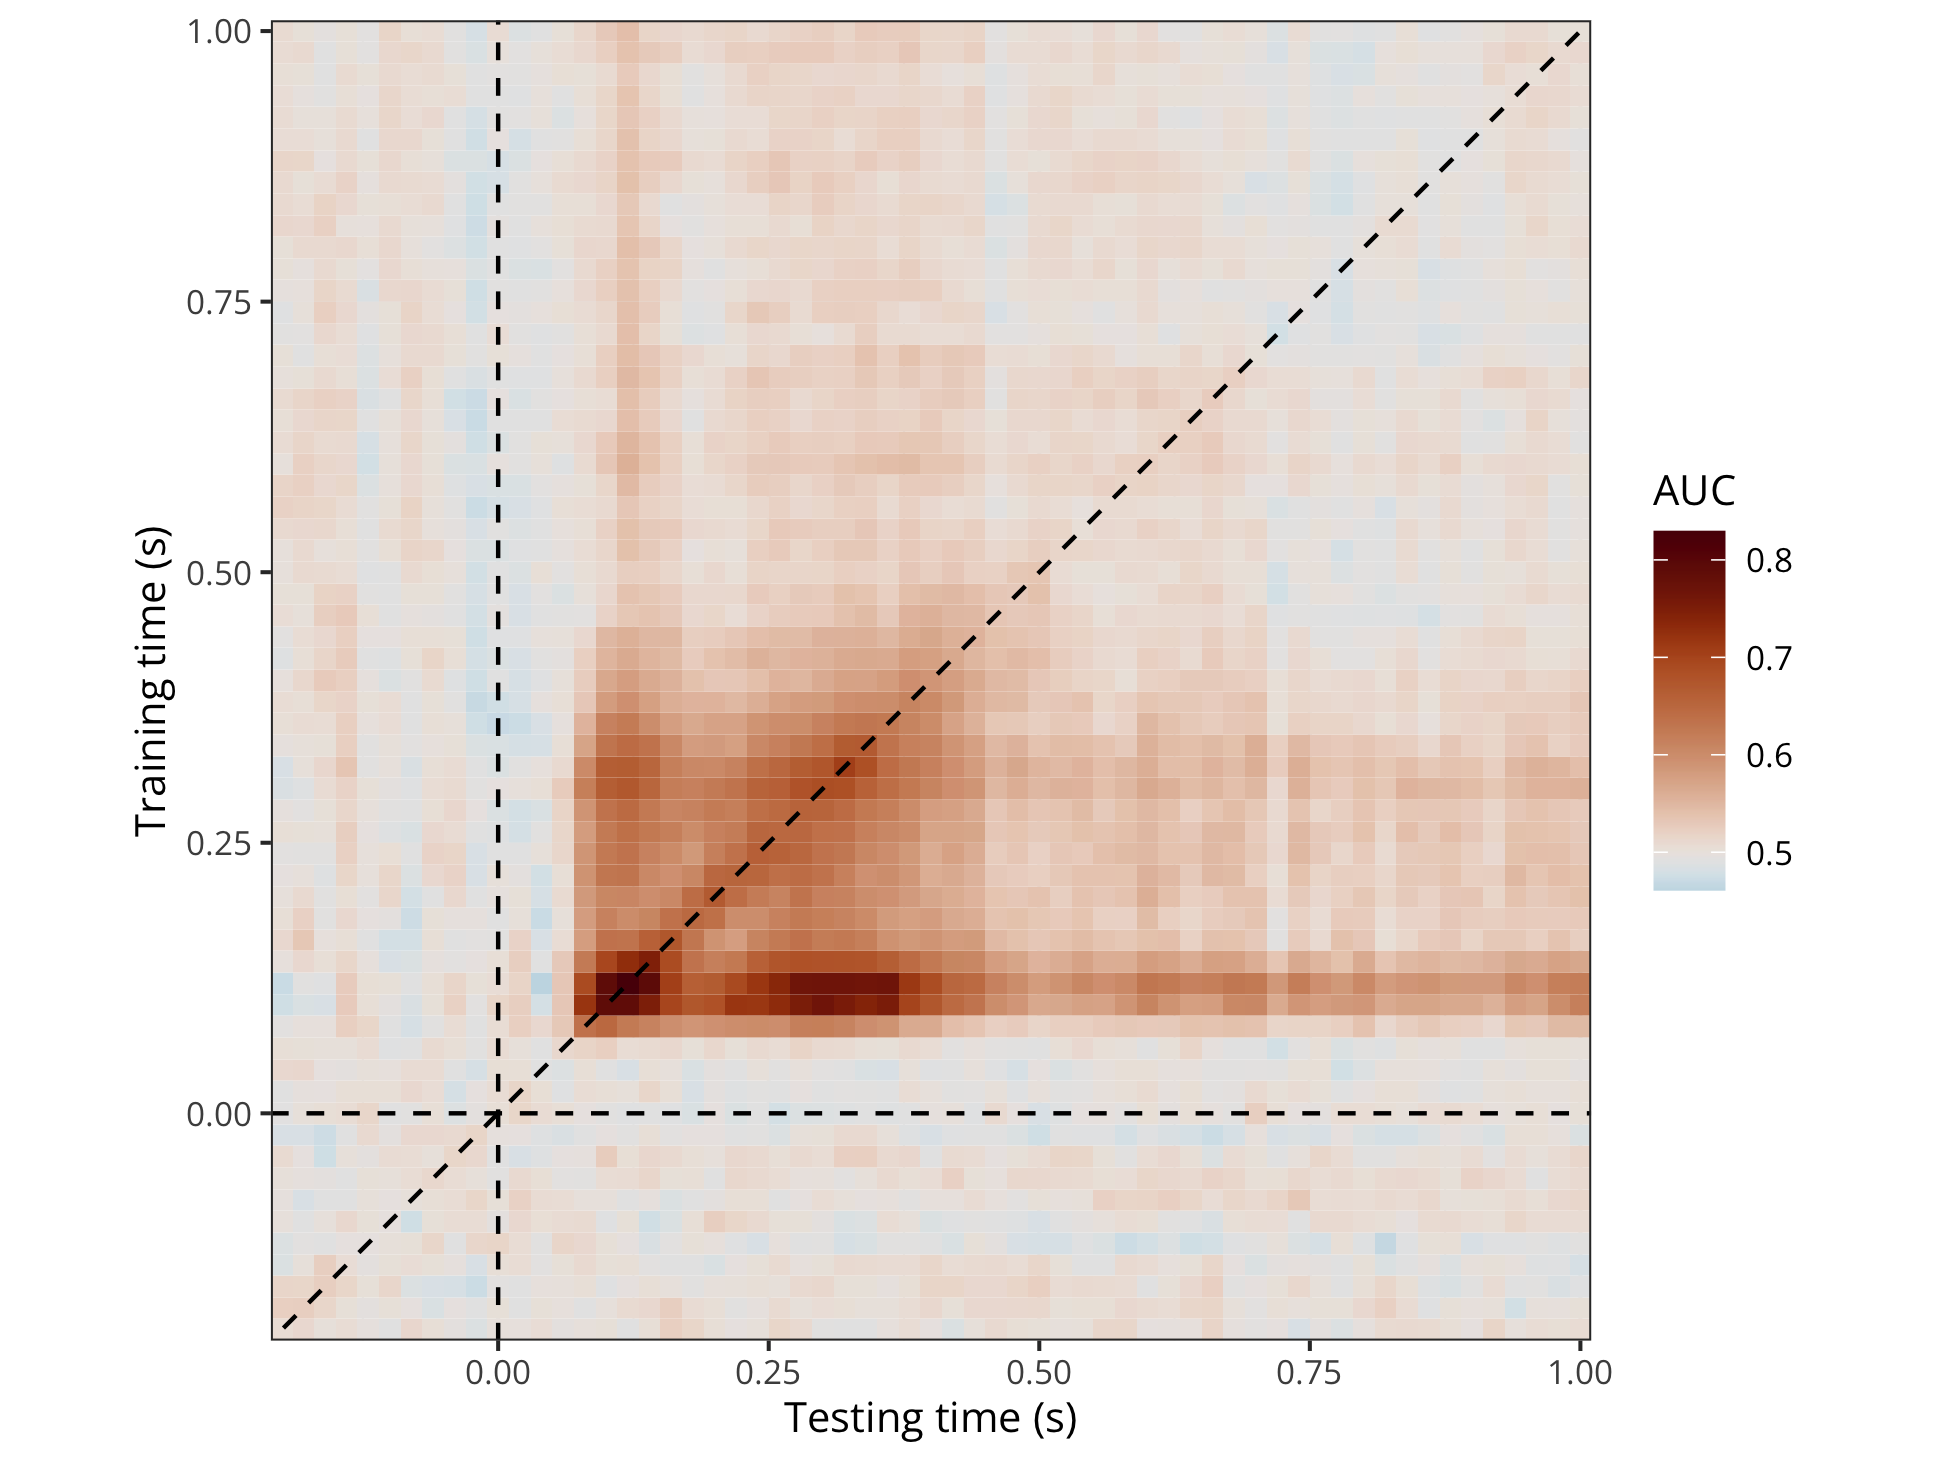
\includegraphics[width=0.75\textwidth,height=\textheight]{manuscript_files/figure-pdf/fig-timegen-1.png}

}

\end{figure}%

\setlength{\parindent}{0pt}
\setlength{\parskip}{6pt}

To model cross-temporal generalisation matrices of decoding performance,
we extended our initial BGAM to take into account the bivariate temporal
distribution of AUC values, thus producing naturally smoothed estimates
(timecourses) of AUC values and posterior odds. This model can be
written as follows:

\[
\begin{aligned}
\text{AUC}_{i} &\sim \mathrm{Beta} \left(\mu_{i}, \phi\right)\\
\operatorname{logit} \left(\mu_{i} \right) &= \alpha + f \left(\text{train}_{i}, \text{test}_{i} \right)\\
f \left(\text{train}_{i}, \text{test}_{i} \right) &\equiv \sum_{k=1}^K b_{k} B_{k}\left(\text{train}_{i}, \text{test}_{i} \right)
\end{aligned}
\]

\setlength{\parindent}{0pt}
\setlength{\parskip}{6pt}

where AUC values are assumed to follow a \(\mathrm{Beta}\) distribution,
parametrised by a mean \(\mu_{i}\) and a precision parameter \(\phi\).
The mean \(\mu_{i}\) is linked to the predictors through a logit link
function. The smooth function \(f(\text{train}_{i}, \text{test}_{i})\)
represents a two-dimensional surface defined over training and testing
times, which captures how decoding performance varies across the
temporal generalisation matrix. This surface is approximated by a linear
combination of \(K\) basis functions \(B_{k}(\cdot, \cdot)\), each
weighted by a coefficient \(b_{k}\). The basis functions are constructed
using a tensor product of univariate splines (here thin-plate splines)
applied to the training and testing time dimensions
(\citeproc{ref-wood2003}{Wood, 2003a}, \citeproc{ref-wood2017}{2017a}).

\setlength{\parindent}{0pt}
\setlength{\parskip}{6pt}

We fitted this model using \texttt{brms} and the \texttt{t2()} tensor
product smooth constructor with full penalties
(\citeproc{ref-pedersen_hierarchical_2019}{E. J. Pedersen et al., 2019};
\citeproc{ref-wood2017}{Wood, 2017a}). We ran eight MCMCs to approximate
the posterior distribution, including each 5000 iterations and a warmup
of 1000 iterations, yielding a total of \(8 \times (5000-1000) = 32000\)
posterior samples to be used for inference.

\begin{Shaded}
\begin{Highlighting}[]
\CommentTok{\# fitting a GAM with two temporal dimensions}
\NormalTok{timegen\_gam }\OtherTok{\textless{}{-}} \FunctionTok{brm}\NormalTok{(}
    \CommentTok{\# 2D thin{-}plate spline (tp) with full penalties}
\NormalTok{    auc }\SpecialCharTok{\textasciitilde{}} \FunctionTok{t2}\NormalTok{(train\_time, test\_time, }\AttributeTok{bs =} \StringTok{"tp"}\NormalTok{, }\AttributeTok{k =} \DecValTok{30}\NormalTok{, }\AttributeTok{full =} \ConstantTok{TRUE}\NormalTok{),}
    \AttributeTok{data =}\NormalTok{ timegen\_data,}
    \AttributeTok{family =} \FunctionTok{Beta}\NormalTok{(),}
    \AttributeTok{warmup =} \DecValTok{1000}\NormalTok{,}
    \AttributeTok{iter =} \DecValTok{5000}\NormalTok{,}
    \AttributeTok{chains =} \DecValTok{8}\NormalTok{,}
    \AttributeTok{cores =} \DecValTok{8}\NormalTok{,}
    \AttributeTok{control =} \FunctionTok{list}\NormalTok{(}\AttributeTok{adapt\_delta =} \FloatTok{0.95}\NormalTok{, }\AttributeTok{max\_treedepth =} \DecValTok{15}\NormalTok{)}
\NormalTok{    )}
\end{Highlighting}
\end{Shaded}

\begin{figure}[!htb]

\caption{\label{fig-gam-timegen-post-preds}Predicted AUC values with
threshold (left) and posterior odds of decoding accuracy being above
chance (right) according to the bivariate BGAM.}

\centering{

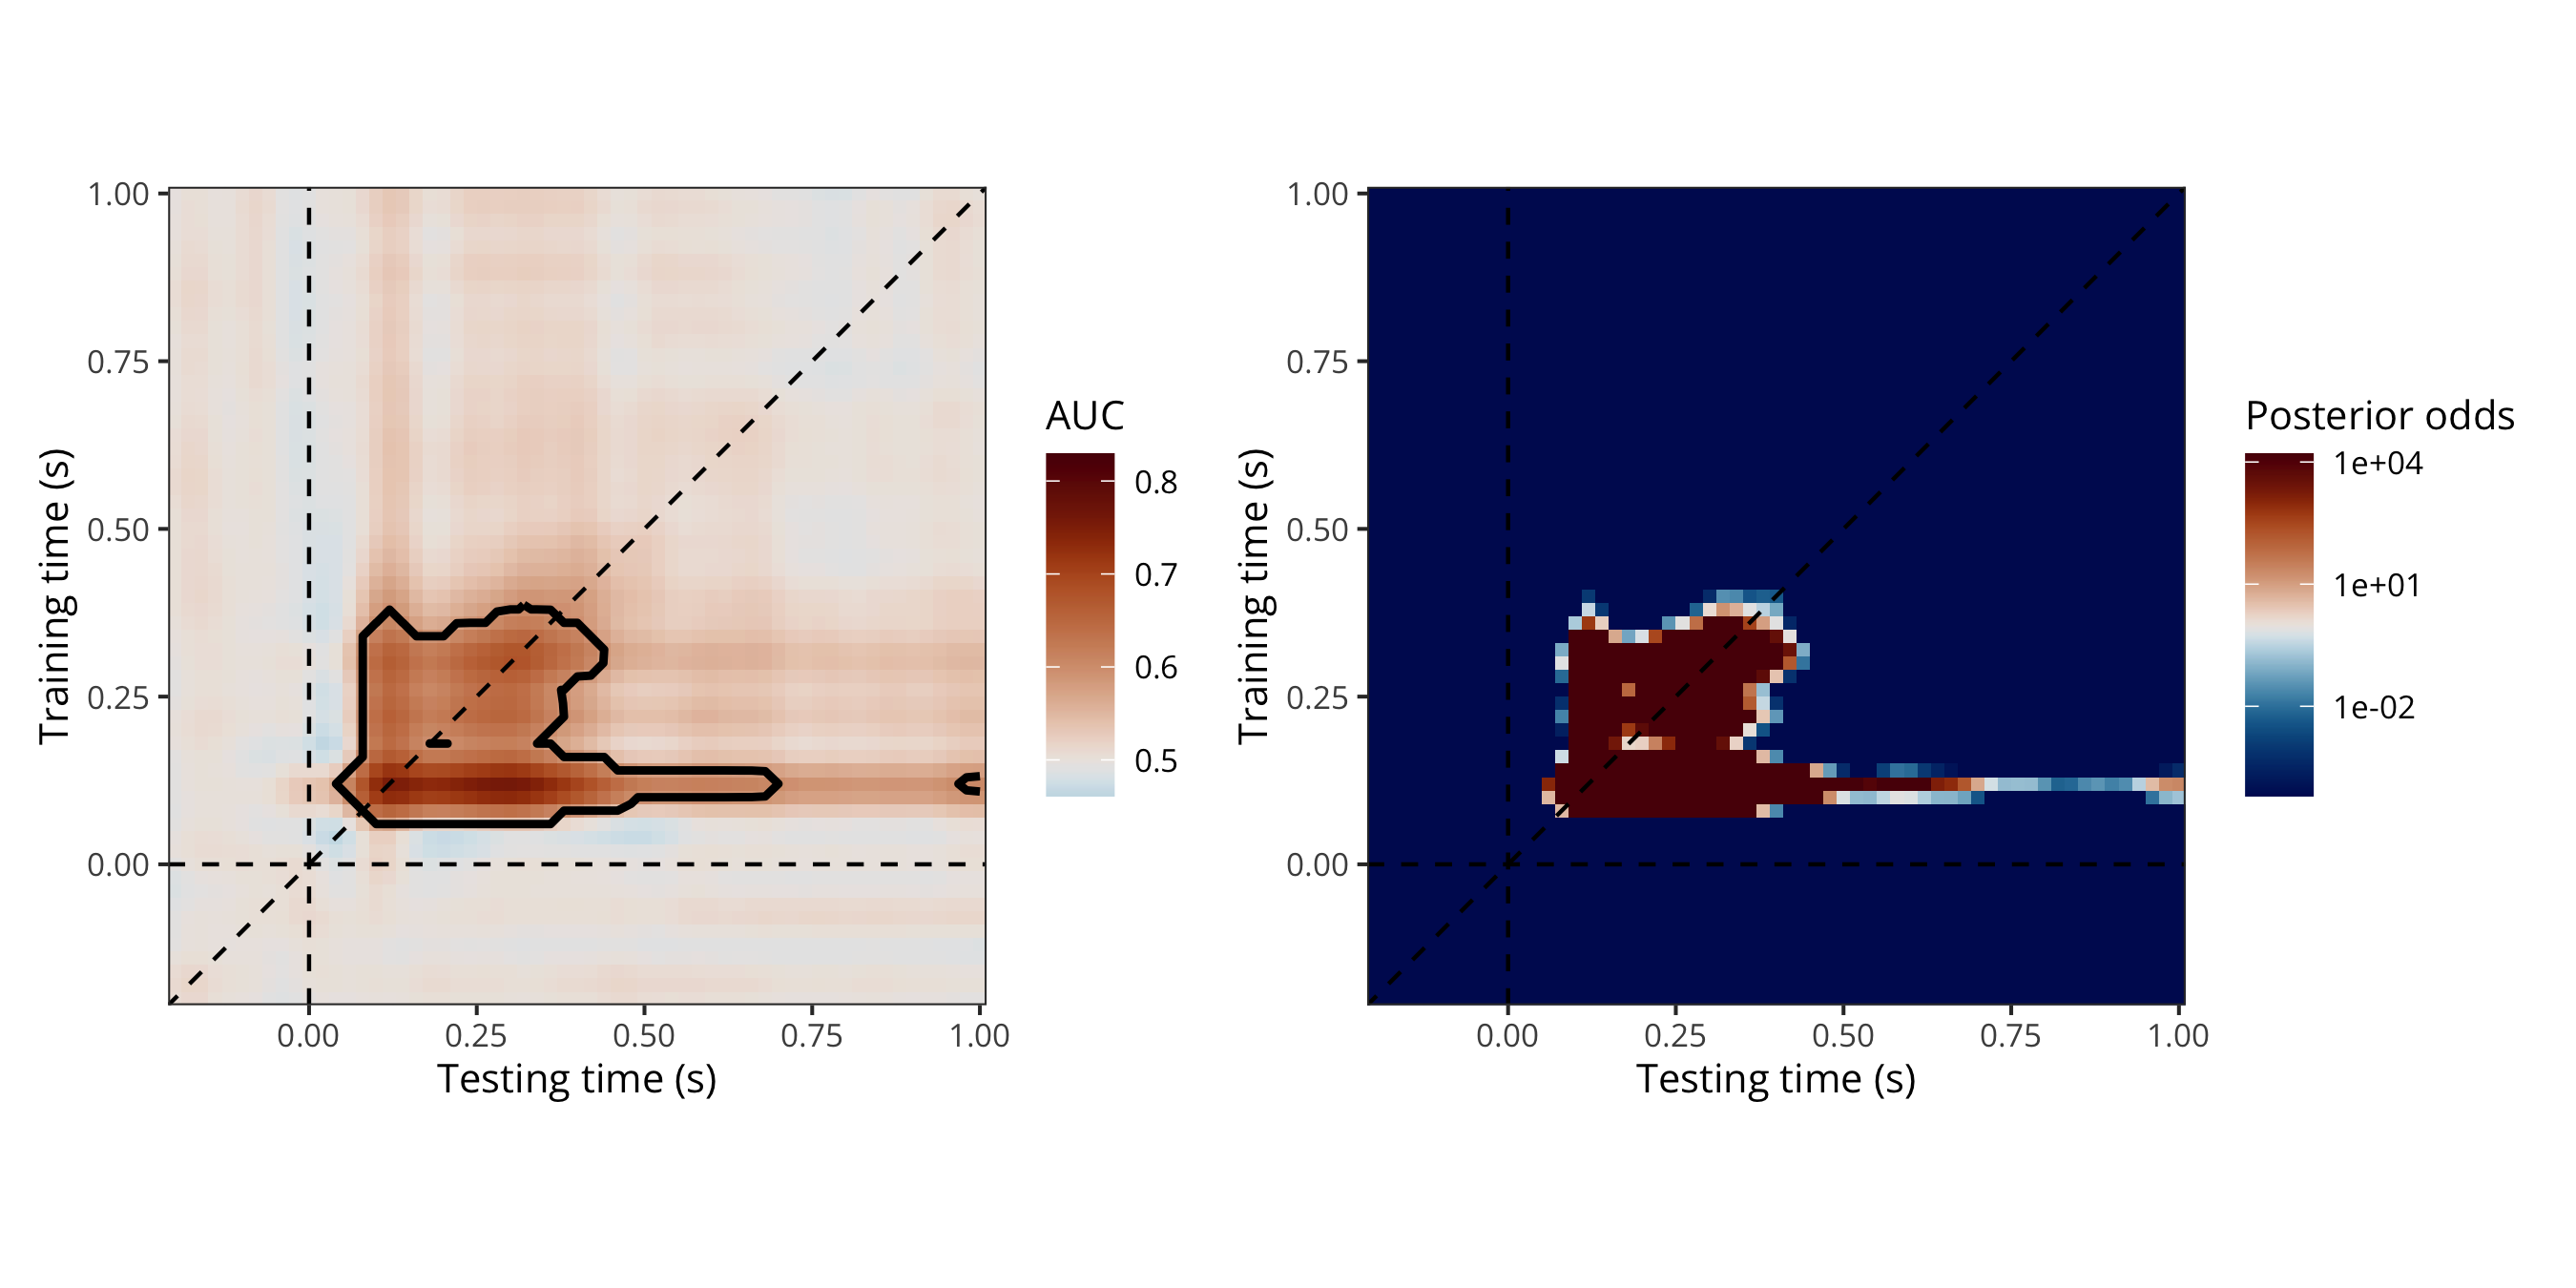
\includegraphics[width=1\textwidth,height=\textheight]{manuscript_files/figure-pdf/fig-gam-timegen-post-preds-1.png}

}

\end{figure}%

\setlength{\parindent}{0pt}
\setlength{\parskip}{6pt}

Figure~\ref{fig-gam-timegen-post-preds} shows the predictions from the
model (left) superimposed with the identified cluster as defined by
thresholding the posterior odds (right). Notably, this model could be
extended to a multilevel bivariate GAM via
\texttt{t2(train\_time,\ test\_time,\ participant,\ bs\ =\ c("tp",\ "tp",\ "re"),\ m\ =\ 2,\ full\ =\ TRUE)}
and could be generalised to account for both spatial (\texttt{x} and
\texttt{y}) and temporal (\texttt{time}) dimensions with formulas such
as \texttt{te(x,\ y,\ time,\ d\ =\ c(2,\ 1)\ )}.

\newpage

\section{How to choose the GAM basis dimension?}\label{apx-basis}

\setlength{\parindent}{0pt}
\setlength{\parskip}{6pt}

There is no universal recommendation for choosing the optimal value of
\texttt{k}, as it depends on several factors, including the sampling
rate, preprocessing steps (e.g., signal-to-noise ratio, low-pass
filtering), and the underlying neural dynamics of the phenomenon under
investigation. One strategy is to set \texttt{k} as high as
computational constraints allow, as suggested by previous authors (e.g.,
\citeproc{ref-pedersen_hierarchical_2019}{E. J. Pedersen et al., 2019}).
Alternatively, one can fit a series of models with different \texttt{k}
values and compare them using information criteria such as LOOIC or
WAIC, alongside posterior predictive checks (PPCs), to select the model
that best captures the structure of the data. We illustrate this
approach below.

\setlength{\parindent}{0pt}
\setlength{\parskip}{6pt}

Figure~\ref{fig-choose-k} presents the posterior predictions and two
forms of posterior predictive checks (PPCs) for each GAM fit using
different numbers of basis functions (\(k \in \{5, 10, 20, 40, 80\}\)).
With the exception of the \(k=5\) model, all other fits yield
satisfactory PPCs, indicating that the predicted data closely resemble
the empirical observations. However, model comparison using the
leave-one-out information crtierio (LOOIC), as summarised in
Table~\ref{tbl-simulation-results}, identifies the \(k=40\) model as the
best-performing one in terms of LOOIC, closely followed by the \(k=80\)
model. This suggests that the optimal number of basis functions likely
lies between these two values. Future simulation studies could further
investigate how such model selection criteria relate to the precision of
onset and offset estimates.

\begin{table}

{\caption{{Models comparison with LOOIC. Models are arranged by the
diffence in expected log-pointwise density (ELPD) to the best model
(i.e., k=40).}{\label{tbl-k-results}}}}

\fontsize{7.5pt}{9.0pt}\selectfont
\begin{tabular*}{\linewidth}{@{\extracolsep{\fill}}lcccccccc}
\toprule
k & elpd\_diff & se\_diff & elpd\_loo & se\_elpd\_loo & p\_loo & se\_p\_loo & looic & se\_looic \\ 
\midrule\addlinespace[2.5pt]
40 & 0.00 & 0.00 & 5,579.11 & 69.47 & 47.79 & 0.74 & -11,158.21 & 138.94 \\ 
80 & -0.63 & 0.38 & 5,578.47 & 69.48 & 50.30 & 0.78 & -11,156.94 & 138.97 \\ 
20 & -6.43 & 3.38 & 5,572.68 & 69.59 & 36.99 & 0.58 & -11,145.35 & 139.17 \\ 
10 & -36.12 & 8.85 & 5,542.98 & 69.88 & 19.29 & 0.32 & -11,085.97 & 139.76 \\ 
5 & -1,605.12 & 53.40 & 3,973.99 & 71.54 & 11.13 & 0.19 & -7,947.98 & 143.09 \\ 
\bottomrule
\end{tabular*}

\end{table}

\begin{figure}[!htb]

\caption{\label{fig-choose-k}Posterior predictions and posterior
predictive checks for the GAM with varying k (in rows).}

\centering{

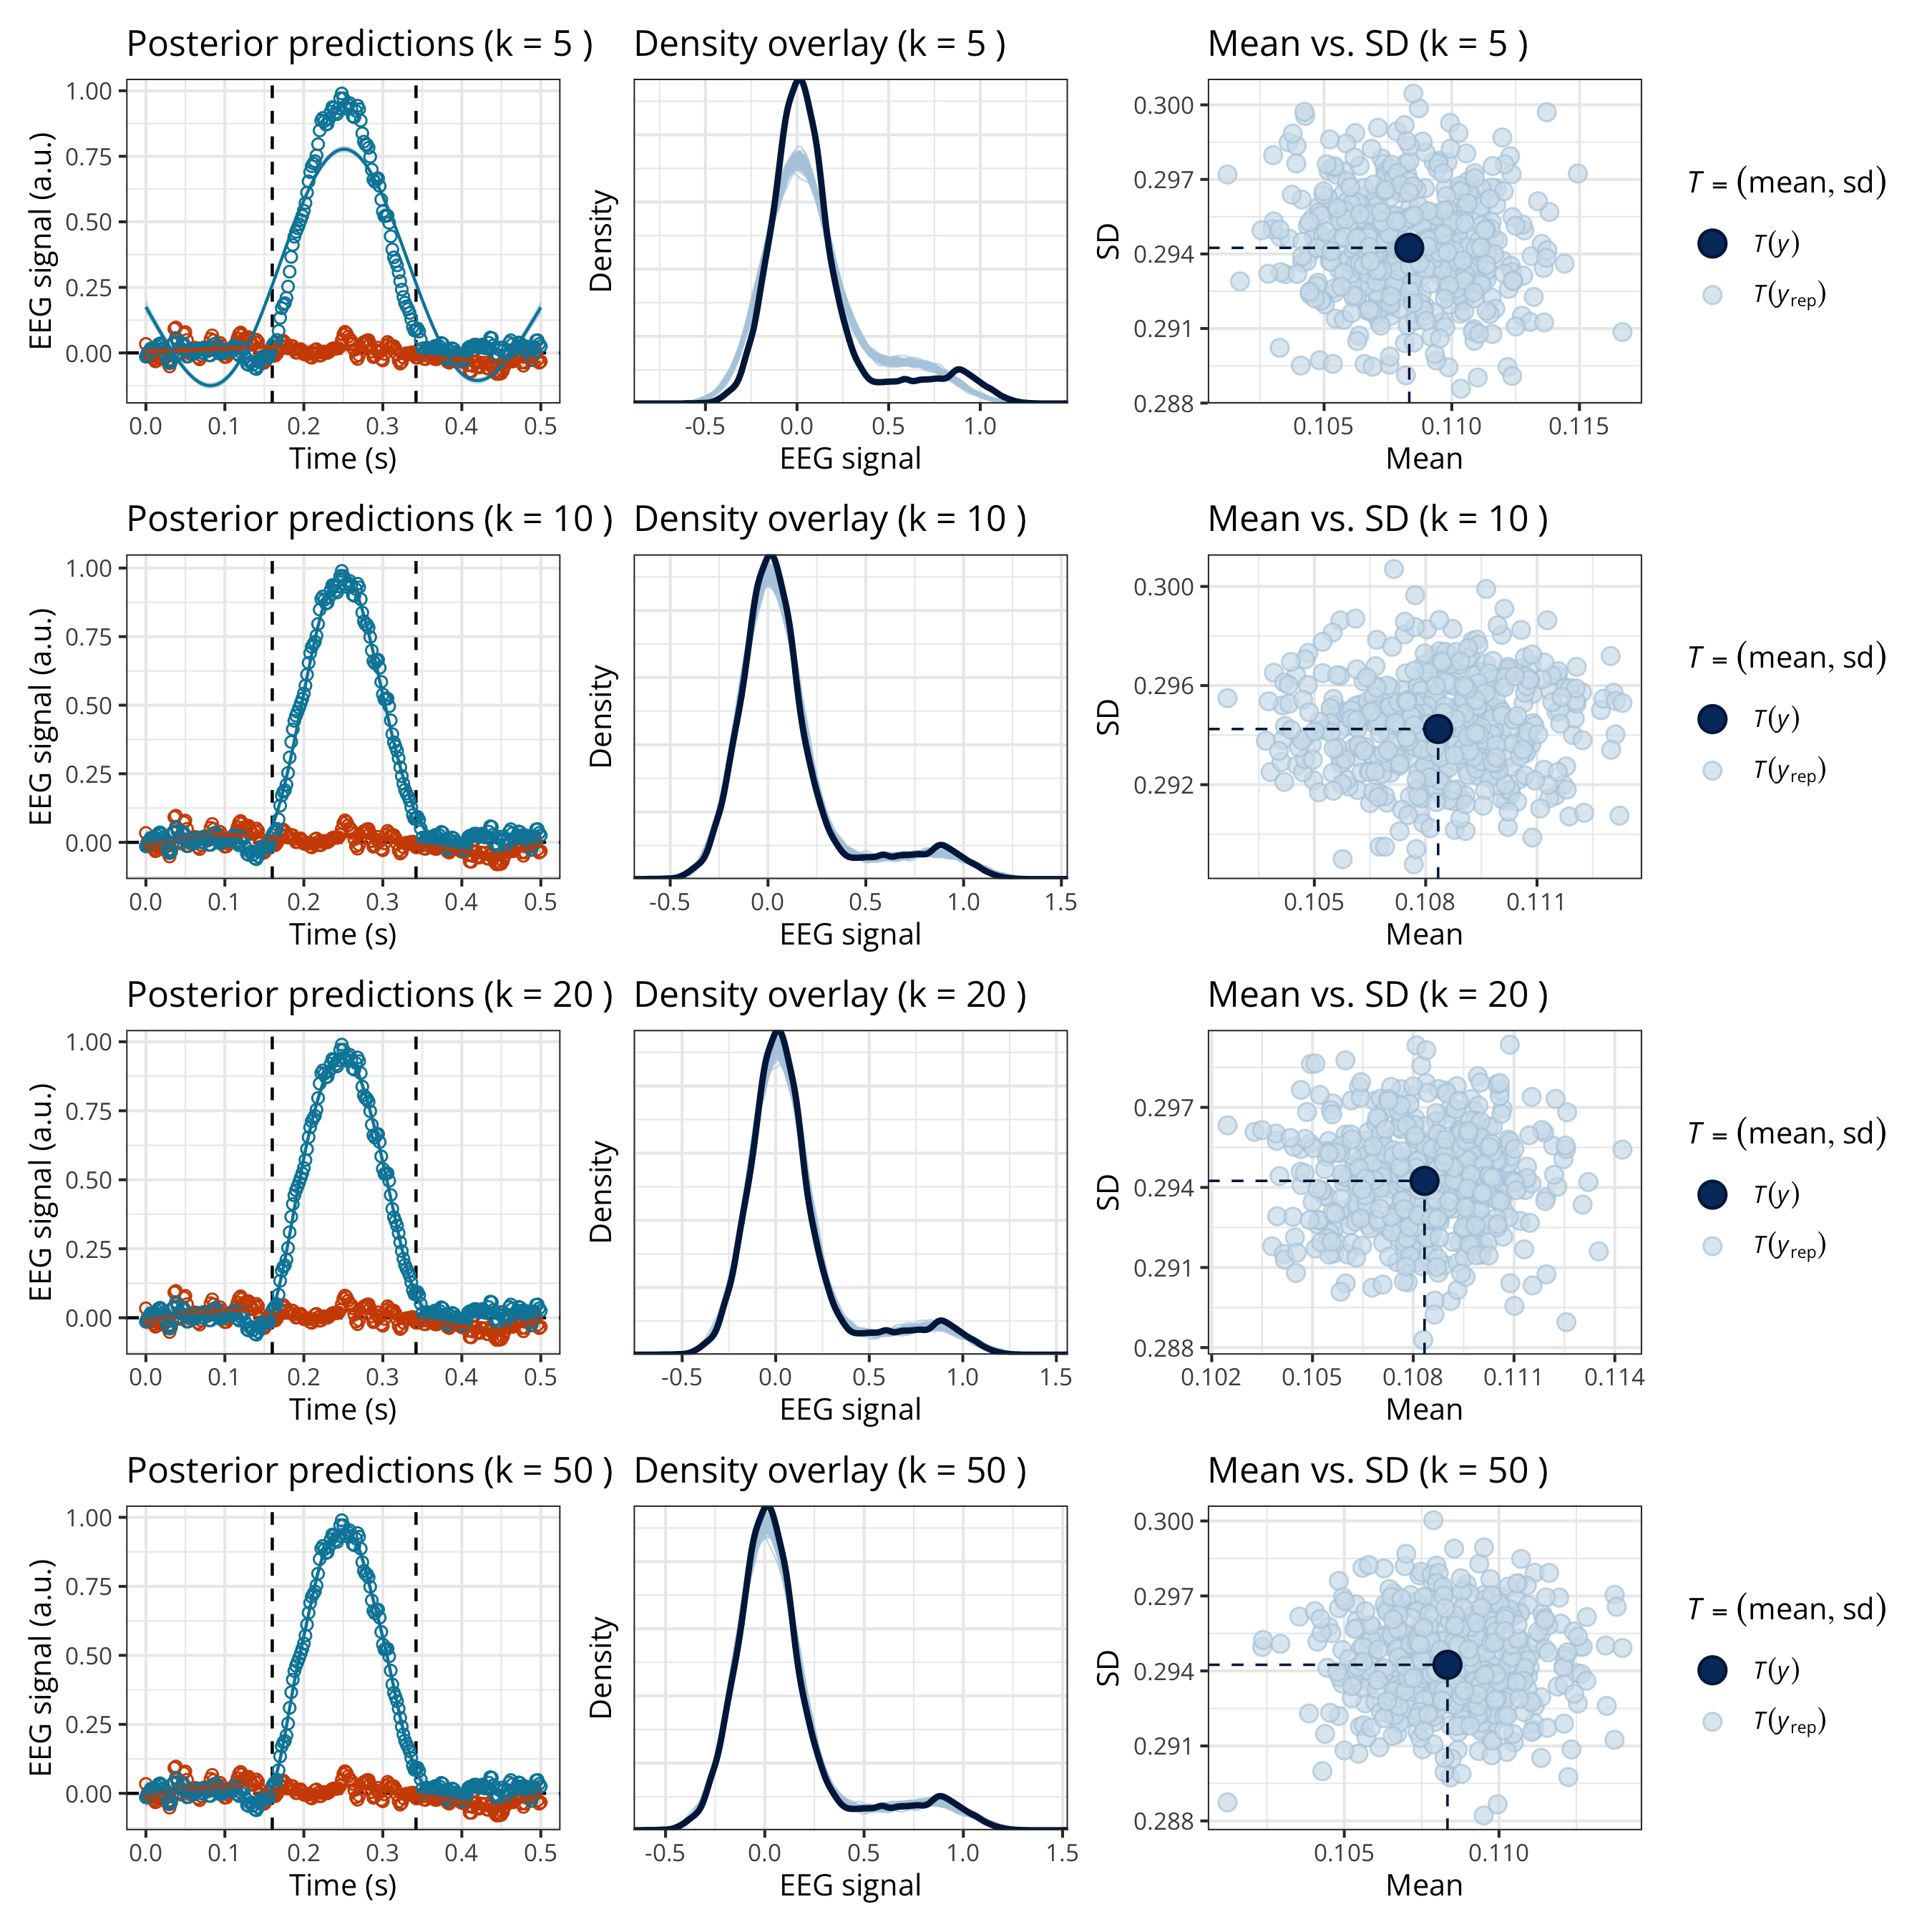
\includegraphics[width=1\textwidth,height=\textheight]{manuscript_files/figure-pdf/fig-choose-k-1.png}

}

\end{figure}%

\clearpage
\thispagestyle{empty}
\null

\section{\texorpdfstring{\texttt{R} package and integration with
\texttt{MNE-Python}}{R package and integration with MNE-Python}}\label{apx-package}

\setlength{\parindent}{0pt}
\setlength{\parskip}{6pt}

For readers who are already familiar with \texttt{brms}, the recommended
pipeline is to use the code provided in the main paper (available at
\url{https://github.com/lnalborczyk/brms_meeg}). It is also possible to
call functions from the \texttt{neurogam\ R} package (available at
\url{https://github.com/lnalborczyk/neurogam}) which come with sensible
defaults.

\begin{Shaded}
\begin{Highlighting}[]
\CommentTok{\# installing (if needed) and loading the neurogam R package}
\CommentTok{\# remotes::install\_github("https://github.com/lnalborczyk/neurogam")}
\FunctionTok{library}\NormalTok{(neurogam)}

\CommentTok{\# using the testing\_through\_time() function from the neurogam package}
\CommentTok{\# this may take a few minutes (or hours depending on the machine\textquotesingle{}s}
\CommentTok{\# performance and the size of the dataset)...}
\NormalTok{gam\_onset\_offset }\OtherTok{\textless{}{-}} \FunctionTok{testing\_through\_time}\NormalTok{(}
    \CommentTok{\# dataframe with M/EEG data in long format}
    \AttributeTok{data =}\NormalTok{ raw\_df,}
    \CommentTok{\# the *\_id arguments are used to specify the relevant columns in data }
    \AttributeTok{participant\_id =} \StringTok{"participant"}\NormalTok{, }\AttributeTok{meeg\_id =} \StringTok{"eeg"}\NormalTok{,}
    \AttributeTok{time\_id =} \StringTok{"time"}\NormalTok{, }\AttributeTok{predictor\_id =} \StringTok{"condition"}\NormalTok{,}
    \CommentTok{\# posterior odds threshold for defining clusters (20 by default)}
    \AttributeTok{threshold =} \DecValTok{20}\NormalTok{,}
    \CommentTok{\# number of warmup MCMC iterations}
    \AttributeTok{warmup =} \DecValTok{1000}\NormalTok{,}
    \CommentTok{\# total number of MCMC iterations}
    \AttributeTok{iter =} \DecValTok{5000}\NormalTok{,}
    \CommentTok{\# number of MCMCs}
    \AttributeTok{chains =} \DecValTok{4}\NormalTok{,}
    \CommentTok{\# number of parallel cores to use for running the MCMCs}
    \AttributeTok{cores =} \DecValTok{4}
\NormalTok{    )}

\CommentTok{\# displaying the results}
\NormalTok{gam\_onset\_offset}\SpecialCharTok{$}\NormalTok{clusters}
\end{Highlighting}
\end{Shaded}

\setlength{\parindent}{0pt}
\setlength{\parskip}{6pt}

The \texttt{neurogam} package can also be called from \texttt{Python}
using the \texttt{rpy2} module, and can easily be integrated into
\texttt{MNE-Python} pipelines. For example, we use it below to estimate
the onset and offset of effects for one EEG channel from an MNE evoked
object. The code used to reshape the \texttt{sample\ MNE} dataset is
available in the online supplementary materials, and we further refer to
the
\href{https://mne.tools/stable/auto_tutorials/epochs/50_epochs_to_data_frame.html}{MNE
documentation} about converting \texttt{MNE} epochs to \texttt{Pandas}
dataframes in long format (i.e., with one observation per row).

\begin{Shaded}
\begin{Highlighting}[]
\CommentTok{\# loading the Python modules}
\ImportTok{import}\NormalTok{ rpy2.robjects }\ImportTok{as}\NormalTok{ robjects}
\ImportTok{from}\NormalTok{ rpy2.robjects.packages }\ImportTok{import}\NormalTok{ importr}
\ImportTok{from}\NormalTok{ rpy2.robjects }\ImportTok{import}\NormalTok{ pandas2ri}
\ImportTok{from}\NormalTok{ rpy2.robjects.conversion }\ImportTok{import}\NormalTok{ localconverter}

\CommentTok{\# importing the "neurogam" R package}
\NormalTok{neurogam }\OperatorTok{=}\NormalTok{ importr(}\StringTok{"neurogam"}\NormalTok{)}

\CommentTok{\# activating automatic pandas{-}R conversion}
\NormalTok{pandas2ri.activate()}

\CommentTok{\# assuming reshaped\_df is some M/EEG data reshaped in long format}
\ControlFlowTok{with}\NormalTok{ localconverter(robjects.default\_converter }\OperatorTok{+}\NormalTok{ pandas2ri.converter):}
    
\NormalTok{    reshaped\_df\_r }\OperatorTok{=}\NormalTok{ robjects.conversion.py2rpy(reshaped\_df)}
    

\CommentTok{\# using the testing\_through\_time() function from the neurogam R package}
\NormalTok{gam\_onset\_offset }\OperatorTok{=}\NormalTok{ neurogam.testing\_through\_time(}
\NormalTok{    data}\OperatorTok{=}\NormalTok{reshaped\_df\_r,}
\NormalTok{    threshold}\OperatorTok{=}\DecValTok{20}\NormalTok{,}
\NormalTok{    multilevel}\OperatorTok{=}\VariableTok{False}
\NormalTok{    )}

\CommentTok{\# displaying the results}
\BuiltInTok{print}\NormalTok{(}\BuiltInTok{list}\NormalTok{(gam\_onset\_offset) )}
\end{Highlighting}
\end{Shaded}







\end{document}
